\chapter{Search for long-lived HNL in final states
with three charged leptons and displaced vertices} \label{Chapter6} 

\section{Change of scenario}
While the SM is in excellent agreement with the LHC measurements, many problems
should be still resolved.

So far an explicit signal of New Physics from either direct or indirect
searches at the LHC, or direct detection of Dark Matter is
missing. Furthermore, theory presents no clear direction on the New Physics scale.
This forces a refining and widening of the experimental effort in the
investigation for New Physics. We should explore various ranges of
interaction strengths and masses in addition with respect to
what is already probed and explored by the current experimental
settings and analysis.

Among the plethora of possible new physics theories, quite eccentric
possibilities of new particles could long-lived particles (LLPs)
decaying in the detector or long-lived detector-stable particle which decay outside the detector volume. 
These two require a change of scenario with respect to the usual SM
prompt searches probed till these days and they do require the
inclusion of unconventional signature searches.

Long-lived particles could be foreseen by several models due to:
\begin{itemize}
\setlength\itemsep{-0.1em}
\item \emph{small coupling constants} -- \ie RPV SUSY (R-parity violating
  SUSY scenario), HNL, etc;
\item \emph{very off-shell intermediate decay products} -- \ie split SUSY where
heavy intermediate squarks enhance
the gluino lifetime~\cite{ATLAS-CONF-2019-006,2020135114};
\item \emph{limited decay phase space} --- \ie
anomaly mediated SUSY breaking
model where the lightest neutralino
and chargino are nearly degenerate~\cite{Sirunyan:2019wau,Sirunyan:2019gut}.
\end{itemize}

CMS and ATLAS were 
initially designed to optimize object
identification for prompt particles, thus to integrate displaced
signatures into CMS framework we have to face quite a diverse number
of challenges:
\begin{itemize}
\setlength\itemsep{-0.1em}
\item \emph{triggers}: timing information at trigger level is not always
  available and the majority of current triggers uses primary vertex
  seeds to identify the matching tracks;
\item \emph{reconstruction}: we need the possibility to use algorithms which
  fit the eventual secondary vertices and adopt such infos in the
  reconstruction procedure;
\item \emph{background}: additional sources of background have to be
  considered such as noise from the detector itself (instrumental
  background), cosmic rays traveling through CMS's barrel, in-time
  and out-of-time pileup and long-lived standard model hadrons which
  could mimic the interesting BSM particle.
\end{itemize}

\subsection{Displaced signature at CMS}
In the sketch in Fig.~\ref{fig:c6antonelli}, several displaced
signatures are shown.

If the
LP decay into charged objects, we can have visible secondary vertices
made either of displaced leptons or of displaced jets; in case the LP decays into two $\gamma$,
then we should rely on the possibility of the CMS
ECAL to measure $\gamma$ arrival times with enough precision to detect
signatures of delayed photons produced at displaced
vertices~\cite{Sirunyan:2019wau}.
There is also the possibility of having the LP that decays within the
volume of the silicon tracker producing events with an isolated track
which "disappears'' \ie it misses hits in the outermost layers of the
silicon tracker, it is associated with little energy deposited in the
calorimeters and it does not show hits in the muon detectors~\cite{Sirunyan_2020disapp}. 
\begin{figure}[h]
\centering
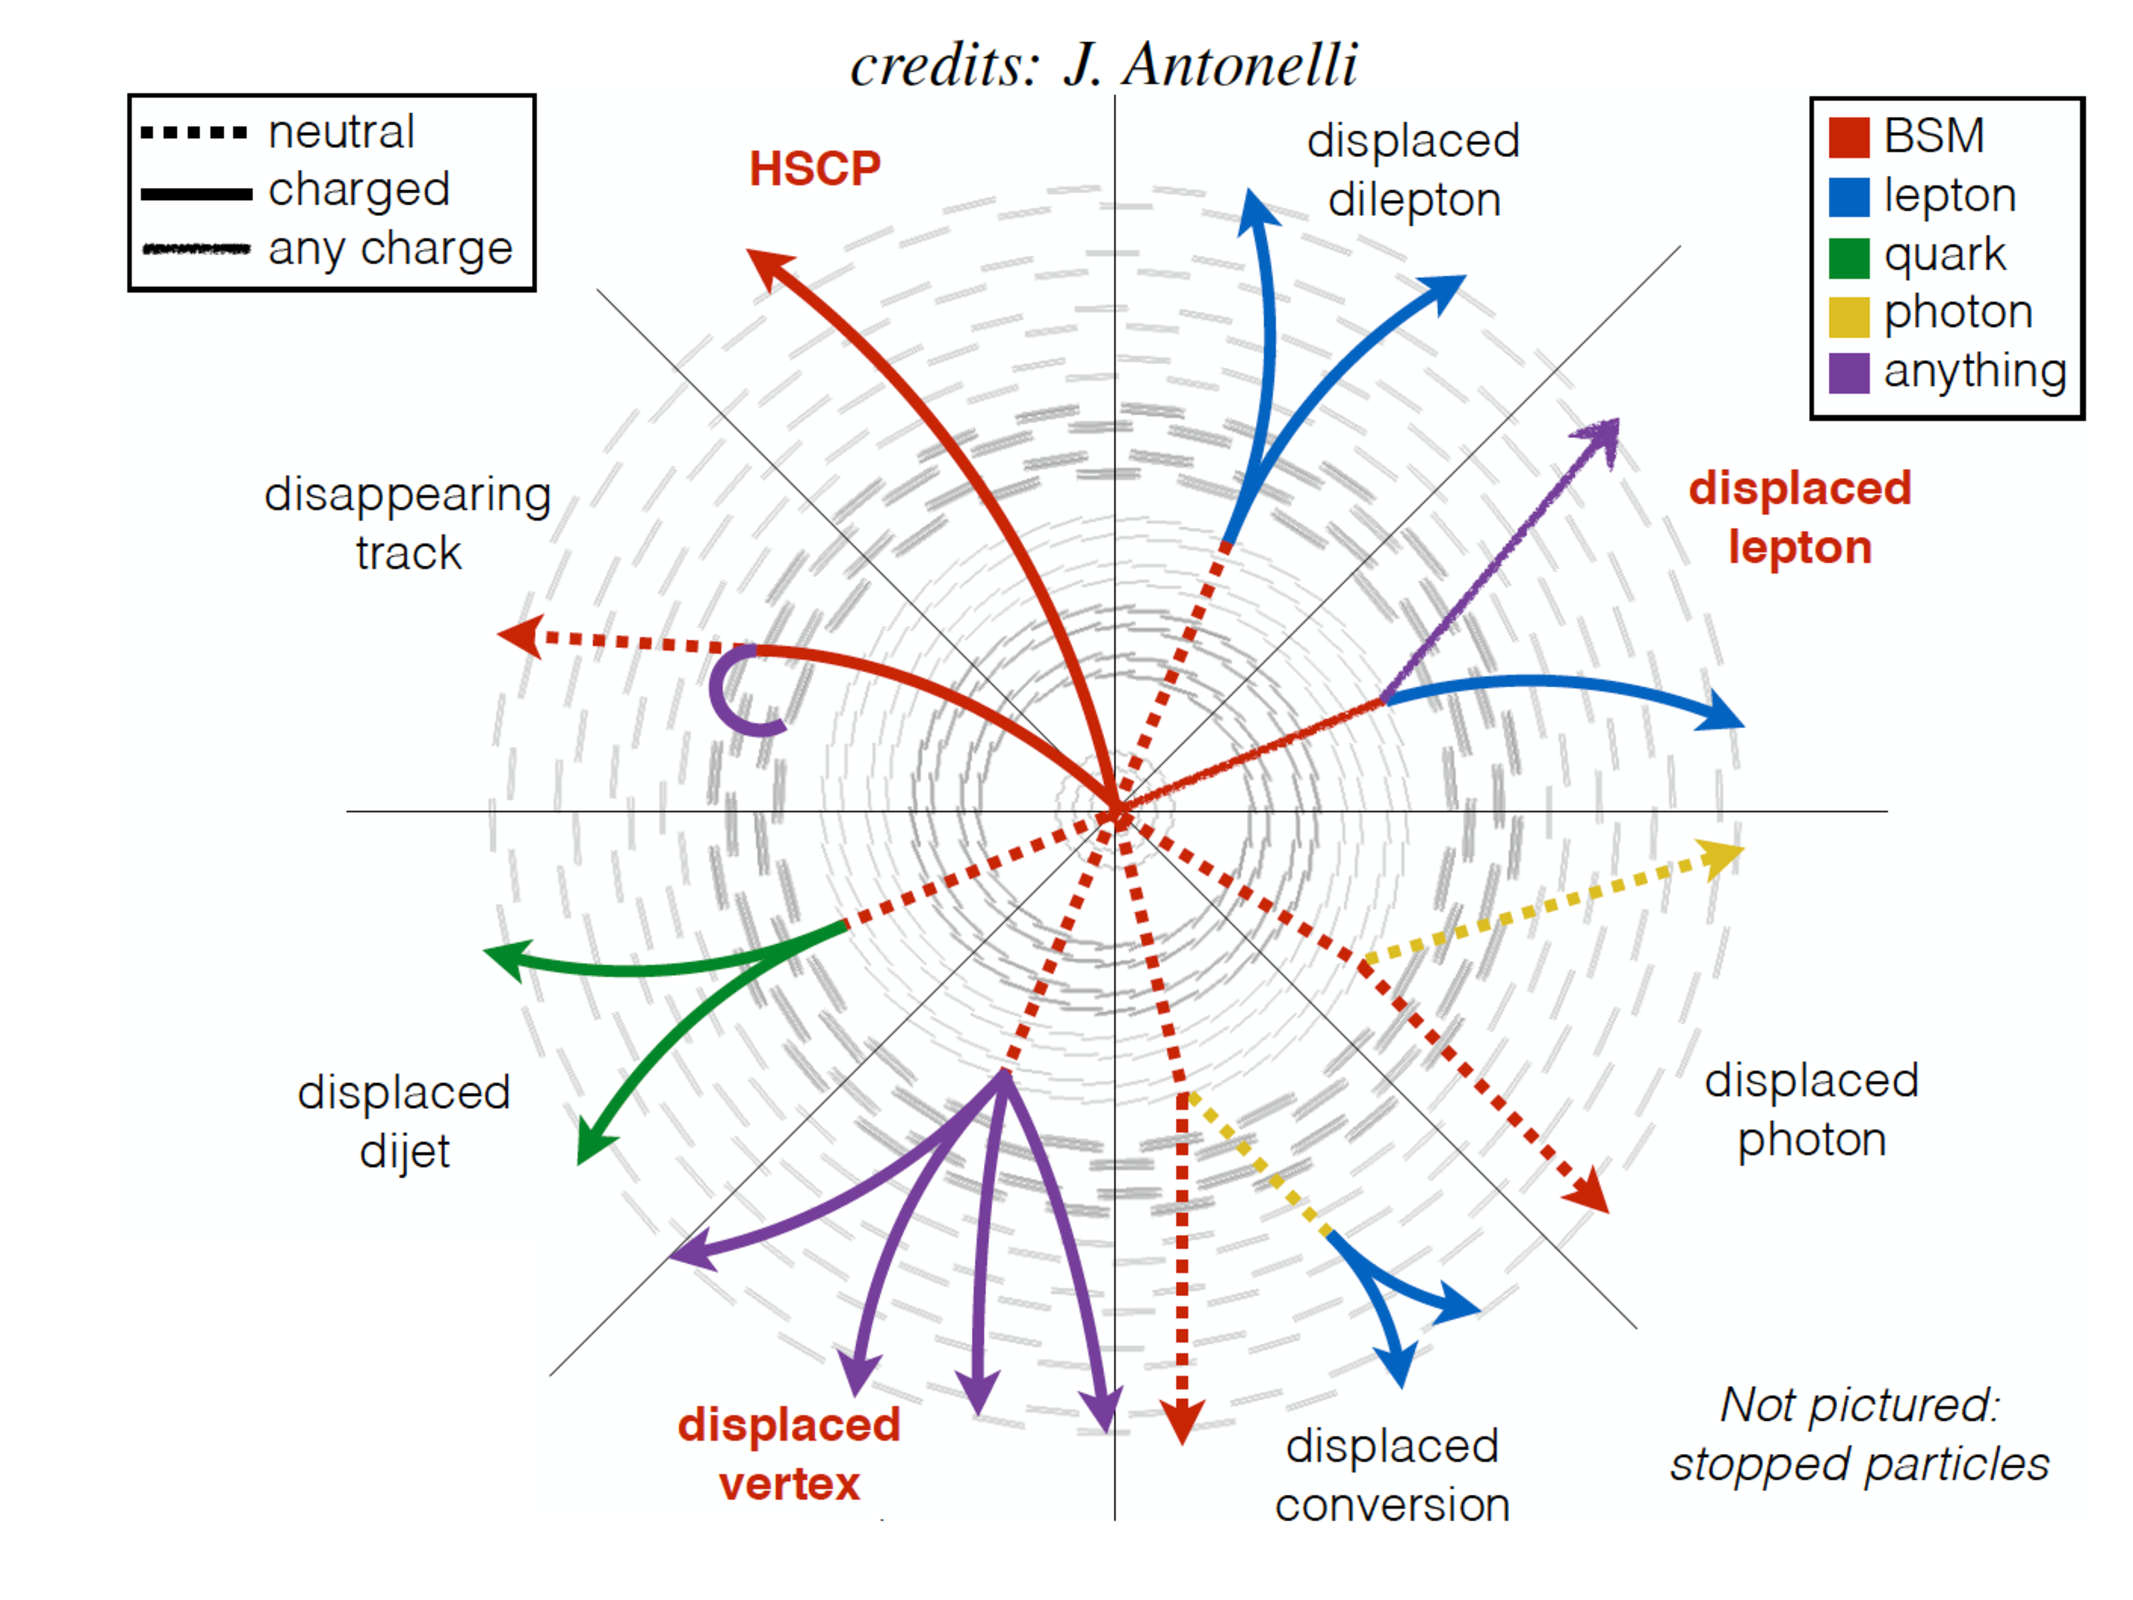
\includegraphics[width=0.85\textwidth]{Figures/c6/antonelli_skech.pdf}
\caption{Didactic sketch, by J. Antonelli, showing the numerous
  Long-lived scenarios which could be seen and probed inside the CMS tracker. }
\label{fig:c6antonelli}
\end{figure}

These are just few examples of the almost endless configurations which can
be studied including the \emph{long-lived} signatures in the
current particle physics searches. 

\subsubsection{Long-lived HNL}
Along these lines, extending the HNL search described in
Chapter~\ref{Chapter5} including the long-lived HNL decays it feels like a logical
continuation. 

Recalling the considerations illustrated in Sec.~\ref{sec:promptll}, the lifetime of a HNL is strongly dependent on \mhnl and \mixpar,
and increases rapidly at small masses and low values of the mixing
parameter (see Fig.~\ref{fig:hnlLifetime}):
\(\tau_\hnl\propto\mathrm{\mhnl^{-5}|V_{\hnl\ell}|^{-2}}.\)
As a result, the kinematics and acceptance of HNLs with masses
below about 20\GeV are significantly affected by their long lifetimes,
and must be accounted for in the signal simulation and in the result
interpretation.
If $\hnl$ has a long lifetime, in particular, its decay products
($\ell^{\pm\prime}$, $\ell^{\mp\prime\prime}$, $\nu_{\ell^{\prime\prime}}$ or
$\nu_{\ell^{\prime}}$, $\ell^{\pm\prime\prime}$, $\ell^{\mp\prime\prime}$)
emerge from a secondary vertex, spatially displaced with respect to
the primary vertex of the process, and distinguishable from it.

We present here the search of long-lived Heavy Neutral Leptons in final states
with three charged leptons and displaced vertices. 

The analysis strategy we follow here shares some similarities with the
prompt HNL search (~\cite{Sirunyan:2018mtv}-Chapter~\ref{Chapter5})
and uses the lessons learned from that
analysis. 
The main objective of the current search is to extend the
sensitivity to low HNL masses and mixing parameters, namely HNL masses
below about 20 GeV. This is obtained by optimizing the identification
of leptons produced in the decay of long-lived HNLs and by fitting
their displaced decay vertices. More precisely, the search is
performed by designing search regions formed by the displacement of
the HNL vertex and the invariant mass of the \displ leptons. The
maximum sensitivity is reached by simultaneously fitting these search
regions in each lepton flavor channels. The mixing of HNL to electron
neutrino, \mixpare, is probed using the leptonic channels 
$\Pe\Pe\Pe$, $\Pepm\Pemp\PGm$, and $\Pepm\Pepm\PGm$ (collectively
called \eex),
while the $\PGm\PGm\PGm$,  $\PGmpm\PGmmp\Pe$, and $\PGmpm\PGmpm\Pe$
channels (collectively called \mmx) are used to probe the coupling to
muon neutrino, \mixparm.
With these lepton flavor/charge configurations, the search is
sensitive to both LNV and LNC scenarios.
The search uses the full Run-II data set with an integrated luminosity
of 137\fbinv, and the major backgrounds are estimated using a
data-driven technique.

%%%%%%%%%%%%%%%%%%%%%%%%%%%%%%%%%%%%%%%%%%%%%%%%%%%%
\section{Analysis setup}
\subsection{Data and simulation samples}
The current analysis uses three sets of $pp$ collision data at a
center-of-mass energy of 13\TeV, corresponding to integrated
luminosities of 35.92\fbinv (2016), 41.53\fbinv (2017), and 59.97\fbinv
(2018). Several primary data sets (PD) are used to search for HNLs decaying
to different lepton flavors, as well as to build control regions for
background estimation:
\begin{itemize}
\setlength\itemsep{-0.1em}
\item SingleElectron (EGamma in 2018);
\item SingleMuon;
\item DoubleEG (EGamma in 2018);
\item DoubleMuon.
\end{itemize}
Possible overlaps among different data sets are
removed by checking run, lumi-section, and event numbers in order to
not have twice the same event coming from different PDs.

Data samples in \texttt{MiniAOD} format are used, including all the
latest/greatest detector and object calibrations available at the time
the analysis is conducted.
To ensure the best quality for the analyzed data, only certified data
events included in the so-called "golden'' JSON files.

This analysis employs Monte Carlo samples generated in the
\texttt{Summer16} (2016), \texttt{Fall17} (2017), and
\texttt{Autumn18} (2018) campaigns.
To reproduce the correct multiplicity of $\Pp$ interactions per
bunch crossing ("pileup'' or PU) observed in data,
simulated minimum-bias events are mixed to the MC signal and
background events, following appropriate PU scenarios for each data
set (2016, 2017, and 2018).
An event re-weighting procedure is applied \textit{a posteriori} to
correct possible residual discrepancies. The luminosity scenario has a 25~ns bunch crossing separation with an
average of about 25 pileup interactions per bunch crossing. 

A number of signal samples were used for the optimization of the
selection and the interpretation of the results, using the modeling
described in Section~\ref{Chapter4}.
Signal samples include HNL decays with three charged leptons and a
neutrino in the final state, coming from both the
$\hnl\to\PW(\ell\PGn)\ell$ and $\hnl\to\PZ(\ell\ell)\PGn$ decay modes
of \hnl.

\subsection{Trigger strategy}\label{sec:trigger}
Every HNL signal event contains one prompt lepton and two (generally)
\displ leptons. Since (most of) the CMS leptonic triggers are
optimized for prompt lepton identification,
we decided for the use of single-electron and single-muon triggers for the
signal selection, as listed in Table~\ref{tab:sgnlTriggers}.
\begin{table}[h]
{\small
  \begin{center}
    \caption{\label{tab:sgnlTriggers} List of triggers used for the
      signal selection in the three data-taking periods.}
      \begin{tabular}{|l|c|c|c|}
      \hline
      \multirow{2}{*}{Primary data set} & \multicolumn{3}{c|}{Trigger name}\\
      \cline{2-4}
      & 2016 & 2017 & 2018 \\
      \hline\hline
      SingleElectron & \texttt{\scriptsize Electron > 27} & \texttt{\scriptsize Electron > 32} & --- \\
      \hline
      EGamma         & --- & --- & \texttt{\scriptsize Electron > 32} \\
      \hline
      \multirow{2}{*}{SingleMuon} & \multirow{2}{*}{\texttt{\scriptsize Muon > 24}} & \texttt{\scriptsize Muon > 24} & \multirow{2}{*}{\texttt{\scriptsize Muon > 24}} \\
      & & \texttt{\scriptsize Muon > 27} & \\
      \hline
    \end{tabular}    
  \end{center}}
\end{table}
The trigger efficiency in  Monte Carlo (MC) samples is corrected
according to the efficiency observed in data, by using per-event scale
factors (SFs) as a function of the prompt lepton \pt and $\eta$.
In order to make this correction possible, the prompt lepton
identified in each event is matched geometrically to the relevant
"trigger lepton'' (\ie, the lepton reconstructed by the CMS
high-level trigger software) that fired the event. Prompt electrons
(muons) must be matched to the trigger electron (muon) that fired one
of the single-electron (-muon) triggers in
Table~\ref{tab:sgnlTriggers}.
The matching is ensured by requiring that the angular distance
\(\Delta R=\sqrt{\left(\Delta\phi\right)^2+\left(\Delta\eta\right)^2}\) 
between the reconstructed trigger lepton and offline lepton be less
than 0.3. This is the same \DR\ cut used to obtain the trigger SFs
with a tag-and-probe method (see Sec.~\ref{sec:triggereff}).

\subsection{Object selection}\label{sec:object}
For the rigorous explanation of the single object reconstruction in
CMS see Chapter~\ref{Chapter2}, section~\ref{sec:reconstruction}.
In the same section the general reconstraction performances of
displaced object is presented; in the coming subsections, we will
present the efficiency of the current object selection for displaced
object using the HNL-signal MC samples. \\

Signal leptons coming from the \PW\ boson are required to originate
from the event's primary $\Pp$ interaction vertex (PV), defined as
the reconstructed vertex with the highest sum of squared transverse
momenta of associated charged particles, plus the \ptmiss.
The distance of closest approach of the lepton track from the event's
PV (impact parameter, IP) is used to evaluate three variables:
the projection of the IP onto the plane transverse to the beam line
(\textbf{transverse impact parameter} $\boldsymbol{\dxy}$),
the projection of the IP along the beam line (\textbf{longitudinal impact
parameter} $\boldsymbol{\dz}$),
and the significance of the IP
($\mathrm{SIP} = \mathrm{IP}/\sigma_{\mathrm{IP}}$,
where $\sigma_{\mathrm{IP}}$ is the uncertainty associated to IP). Signal leptons coming from the HNL decay are selected by requiring a
minimum \dxy value, and do not have additional constraints on \dz nor
on the IP significance (see Tables~\ref{tab:electronSelection} and
\ref{tab:muonSelection}).

Signal leptons are required to be isolated from any hadronic activity
in the event.
An isolation variable (\Irel) is computed as the scalar 
\pt sum of charged hadrons originating from the PV, neutral hadrons,
and photons within a cone of $\Delta R<0.3$ around the lepton
candidate direction at the vertex,
divided by the transverse momentum $\pt^\ell$ of the lepton candidate:
\begin{linenomath}
  \begin{equation}
    \label{eq:irel}
    \Irel = \frac{1}{\pt^\ell}
    \left(\sum_{ch.hadr.}\pt^{\mathrm{PV}} +
    \max{\left[0, \sum_{neu.hadr.}\pt + \sum_{pho.}\pt
        - \rho\cdot A_{\mathrm{eff}}\right]}\right).
  \end{equation}
\end{linenomath}
The term $\rho\cdot A_{\mathrm{eff}}$ is used to mitigate the
contribution of pileup to the isolation calculation: the average
transverse-momentum flow density $\rho$ is calculated in each event
using a ``jet area'' method~\cite{CACCIARI2008119}, and the effective
area $A_{\mathrm{eff}}$ is the geometric area of the isolation cone
times an $\eta$-dependent correction factor that accounts for the
residual dependence of the isolation on pileup.

\subsubsection{Electrons}\label{sec:llelectron}
Electron reconstruction is based on the combination of tracker and
ECAL information in a Gaussian Sum Filter (GSF)
track~\cite{Khachatryan:2015hwa}, which accounts for possible
bremsstrahlung from the electron.
Electrons are reconstructed within the geometrical acceptance of the
CMS tracking system, $|\eta|<2.5$.
Identification criteria based on the electromagnetic shower shape, track
quality, track impact parameters with respect to the primary vertex,
and isolation are used to select signal electrons and reduce the rate
of mis-identified and background electrons (referred to as ``fake
electrons'' hereafter).
The electron selection criteria are summarized in
Table~\ref{tab:electronSelection}. 
Different criteria are applied to identify prompt and \displ
electrons.
\subparagraph {Prompt electrons}
Prompt electrons are identified using a multi-variate discriminator
(EGM POG 90\% working point MVA ID),
must have \pt greater than 30 (32, 32)\GeV in the 2016 (2017, 2018)
data set,
and must be matched to a ``trigger electron'' (see
Sec.~\ref{sec:trigger}).
The offline \pt threshold is driven by the trigger \pt threshold in
each data set, such that the offline cut always falls in the plateau
of the trigger efficiency turn-on curve.
Prompt electrons passing this selection will be referred to as ``tight
prompt electrons'' hereafter.
\subparagraph {Displaced electrons}
\Displ electrons are identified using a cut-based selection (``EGM
POG cut-based Loose ID''), but removing a veto
on photon conversions and a requirement on the maximum number of
missing inner hits, which could affect the efficiency for electrons
not emerging from the primary vertex.
\Displ electrons passing this selection will be referred to as
``tight \displ electrons''.
They must have \pt greater than 7\GeV.
Samples enriched in fake electrons are selected with
identification criteria looser than those used for tight \displ
electrons. These ``loose \displ electrons'' or ``fakeable objects''
(FO) are employed to determine the rate of fake electrons
mis-identified as signal electrons (``fake rate'' or FR).
\begin{table}[h!]
  \centering
  \caption{\label{tab:electronSelection} Requirements for an electron
    to pass each of the defined selection working points.
    Where three values are given for a single variable, they
    correspond to electrons with $\abseta< 0.8$, $0.8<\abseta<1.479$,
    and $1.479<\abseta<2.5$. The cut on the prompt electron MVA
    discriminator depends on the electron \sigeta and \pt. }
  %  \(f(\sigeta,\pt) = \min{\left\{ x_{15}(\sigeta),\,
   %   \max{\left\{x_{25}(\sigeta),\,x_{15}(\sigeta) +
   %     0.1\cdot(x_{25}(\sigeta)-x_{15}(\sigeta)) \cdot
     %   (\pt-15\GeV)\right\}}\right\}},\)\\
   % where $x_{15}(\sigeta) = (0.77,\,0.56,\,0.48)$ and
    %$x_{25}(\sigeta) = (0.52,\,0.11,\,-0.01)$, with the three values
   % applying to the same \abseta bins defined above.}
  \resizebox{1.0\textwidth}{!}{
    \begin{tabular}{c|c|c|c}
      %% \hline
      %% Cut & Tight prompt & Tight \displ & Loose \displ (FO) \\
      %% \hline
      \hline
      Selection name & Tight prompt & Tight \displ & Loose \displ (FO) \\
      \hline
      EGM POG ID & MVA ID --- 90\% w.p. &
      \multicolumn{2}{c}{Modified cut-based Loose ID} \\
      \hline
      \hline
      $\abseta$ & $<2.5$ & $<2.5$ & $<2.5$ \\
      $\pt$ & $>30$--$32\GeV$ & $>7\GeV$ & $>7\GeV$ \\
      $|d_{xy}|$ & $<0.05$ cm & $>0.01$ cm & $>0.01$ cm \\
      $|d_z|$ & $<0.1$ cm & --- & --- \\
      %$\mathrm{SIP_{3D}}$ & $<4$ & --- & --- \\
      \Irel & $<0.1$ & $<0.2$ & $<2.0$ \\
      $\sigma_{i\eta i\eta}$ & --- & $<(0.011,\,0.011,\,0.030)$ & $<(0.011,\,0.011,\,0.030)$ \\
      H/E & --- & $<(0.10,\,0.10,\,0.07)$ & $<(0.10,\,0.10,\,0.07)$ \\
      $\Delta\eta_{\textrm{in}}$ & --- & $<(0.01,\,0.01,\,0.008)$ & $<(0.01,\,0.01,\,0.008)$ \\
      $\Delta\phi_{\textrm{in}}$ & --- & $<(0.04,\,0.04,\,0.07)$ & $<(0.04,\,0.04,\,0.07)$ \\
      $1/E-1/p$ & --- & $<(0.010,\,0.010,\,0.005)$ & $<(0.010,\,0.010,\,0.005)$ \\
      MVA estimator & $>f(\sigeta,\pt)$ & --- & --- \\
      \hline
    \end{tabular}
    }

\end{table}

\subsubsection{Muons}\label{sec:llmuon}
Muons are reconstructed by combining the information of the tracker
and of the muon
spectrometer~\cite{Sirunyan:2018fpa}.
The geometric compatibility between these separate measurements is
used in the further selection of muons. Muons are required to have
$\abseta<2.4$ to fall inside the geometric acceptance of the muon
detector.
All muons considered for analysis must pass the loose working point as
specified by the MUO POG, in addition to a number
of other loose criteria on isolation and their impact parameters with
respect to the PV.
It is also possible to require muons to be synchronized with the bunch
crossing that has triggered, using the time measurements provided by
the muon sub-detectors, the RPCs (``RPC time'' or $t_{\mathrm{RPC}}$)
and the combined measurements of the DTs and CSCs (``combined time''
or $t_{\mathrm{comb}}$)~\cite{muon_oot}.
In particular, $t_{\mathrm{RPC}}$ ($t_{\mathrm{comb}}$) is only used
if it is measured with more than 1 (7) degrees of freedom.
If $t_{\mathrm{RPC}}$ and $t_{\mathrm{comb}}$ are both available,
they must lie within $-10\ns$ and $+10\ns$.
If only $t_{\mathrm{comb}}$ is available, then it must be within
$-45\ns$ and $+20\ns$.
If $t_{\mathrm{comb}}$ is unavailable, no timing requirement is
applied.
This timing requirement is found to be fully efficient for signal
muons. However, we also find that the background from out-of-time
muons is effectively removed by other muon and event selections (as
described in this section and in Section~\ref{sec:selection}), thus
making the timing requirement redundant. For this reason, it is not
applied.  
Muon selection criteria are summarized in
Table~\ref{tab:muonSelection}.

Different selections are applied to prompt and \displ muons.
\subparagraph {Prompt muons}
Prompt muons must pass identification criteria based on track quality
and matching of the inner tracker track with the measurements in the
muon detectors (``MUO POG Medium ID''), must have \pt greater than
25 (28, 25)\GeV in the 2016 (2017, 2018) data set, and must be matched
to a ``trigger muon'' (see Sec.~\ref{sec:dataset}).
As in the case of electrons, the offline \pt cut is driven in each
data set by the trigger \pt threshold.
Prompt muons passing this selection will be referred to as ``tight
prompt muons'' hereafter.
\begin{table}[h!]
  \centering
  \caption{\label{tab:muonSelection} Requirements for a muon
    to pass each of the defined selection working points.}
  \resizebox{1.0\textwidth}{!}{
    \begin{tabular}{r|c|c|c|c}
      %% \hline
      %% \multicolumn{2}{c|}{Cut} & Tight prompt & Tight \displ & Loose \displ (FO) \\
      %% \hline
      \hline
      \multicolumn{2}{c|}{Selection name} & Tight prompt & Tight \displ & Loose \displ (FO) \\
      \hline
      \multicolumn{2}{c|}{MUO POG ID} & Cut-based Medium ID &
      \multicolumn{2}{c}{Modified cut-based Medium ID} \\
      \hline
      \hline
      \multicolumn{2}{c|}{$\abseta$} & $<2.4$ & $<2.4$ & $<2.4$ \\
      \multicolumn{2}{c|}{$\pt$} & $>25$--$28\GeV$ & $>5\GeV$ & $>5\GeV$ \\
      \multicolumn{2}{c|}{$|d_{xy}|$} & $<0.05$ cm & $>0.01$ cm & $>0.01$ cm \\
      \multicolumn{2}{c|}{$|d_z|$} & $<0.1$ cm & $<10$ cm & $<10$ cm \\
      %\multicolumn{2}{c|}{$\mathrm{SIP_{3D}}$} & $<4$ & --- & --- \\
      \multicolumn{2}{c|}{\Irel} & $<0.1$ & $<0.2$ & $<2.0$ \\
      \multicolumn{2}{c|}{Loose ID} & True & True & True \\
      \multicolumn{2}{c|}{Fraction of valid tracker hits} & $>0.8$ & --- & --- \\
      \hline
      \multirow{5}{*}{Global muon} & Global muon fit & True & True & True \\
      & Global track $\chi^2$/dof & $<3$ & --- & --- \\
      & Track--muon matching $\chi^2$/dof & $<12$ & $<12$ & $<12$ \\
      & ``Kink finder'' estimator & $<20$ & $<20$ & $<20$ \\
      & Segment-compatibility estimator & $>0.303$ & $>0.303$ & $>0.303$ \\
      \hline
      Tracker muon & Segment-compatibility estimator & $>0.451$ & $>0.451$ & $>0.451$ \\
      %% \hline
      %% \multicolumn{2}{c|}{Muon timing (NOT USED)} &
      %% \multicolumn{3}{c}{$t_{\mathrm{RPC}},t_{\mathrm{comb}}\in[-10,+10]\ns$
      %%   ~OR~ $t_{\mathrm{comb}}\in[-45,+20]\ns$} \\
      \hline
    \end{tabular}
    }
\end{table}
\subparagraph {Displaced muons}
\Displ muons must pass requirements similar to the Medium ID, but
removing all selections that may reduce the efficiency for muons not
emerging from the primary vertex.
These \displ muons will be referred to as ``tight \displ muons''
and must have \pt greater than 5\GeV.

In addition, ``loose \displ muons'' or ``muon FOs'' are selected
with identification criteria looser than those used for tight
\displ muons, and are employed to determine the muon FR.
\subparagraph{Modified Medium ID for \displ muons}\label{sec:modifiedMedium}

Figure~\ref{fig:modMedium_common}
show the efficiency of the different selections included in the
standard recommended Medium ID for all \displ leptons from HNL
decays (\ltwo and \lthree), for two typical signal scenarios
($\mhnl=4\GeV$, $\mixparm=8.44\times10^{-6}$ and
$\mhnl=8\GeV$, $\mixparm=3\times10^{-7}$),
as a function of the transverse position of the dilepton vertex
(\Deltwod).
In particular, Fig.~\ref{fig:modMedium_common}(A) shows the efficiency of
reconstructing a muon track in the inner tracker, while 
Fig.~\ref{fig:modMedium_common}(B) shows the sequential
efficiencies of the plain PFMuon requirement, Loose ID selection, and
valid tracker hit fraction cut, with respect to the reconstructed
inner-tracker track. It is clear that the efficiency of
this last requirement falls rapidly with increasing HNL
displacement. The valid-hit fraction cut is thus removed from the
\displ-muon Medium ID, and is not applied in the following
efficiencies.
Figure~\ref{fig:modMedium_common}(C) compares the efficiency of the
tracker-muon and global-muon requirements (as described in
Table~\ref{tab:muonSelection}) and their logical OR (\ie, the full
modified Medium ID). The main contribution to the efficiency comes
from the tracker-muon selection, while the addition of the global-muon
selection only increases the overall efficiency by few percent.
Finally, Fig.~\ref{fig:modMedium_common}(D) compares the efficiency of
the full modified Medium ID with the efficiencies obtained by removing
individual cuts from the global-muon definition. None of these cuts
appears to hurt the overall efficiency significantly---the larger
effect is observed for the segment-compatibility cut of 0.303, and it
amounts to 1--2\%. Additionally, none of the cuts on the global-track
variables depends on the displacement.
\begin{figure}[h]
\noindent
\makebox[\textwidth]{  \subfloat[]{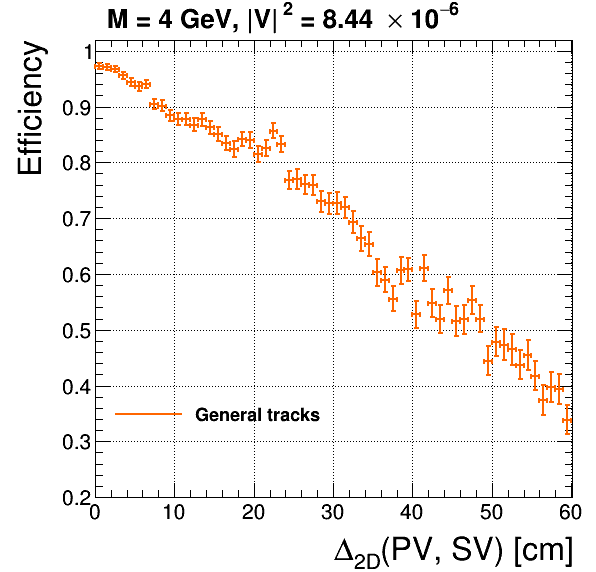
\includegraphics[width=.27\textwidth]{Figures/c6/object/tracking_M-4_V-0p00290516780927_rho.png}
  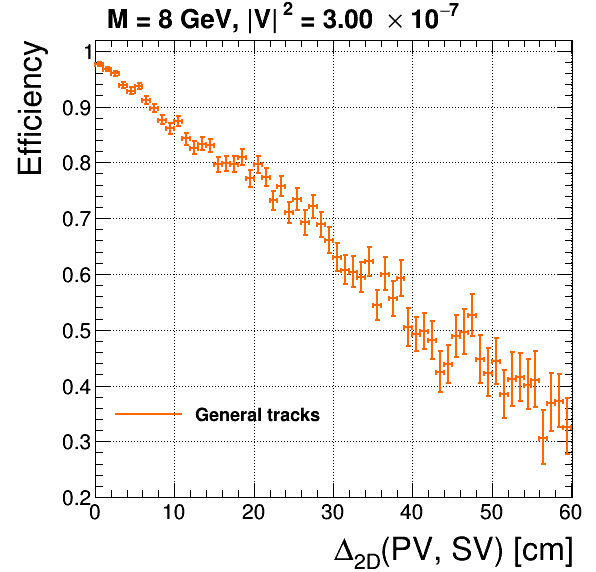
\includegraphics[width=.27\textwidth]{Figures/c6/object/tracking_M-8_V-0p000547722557505_rho.png}}
  \subfloat[]{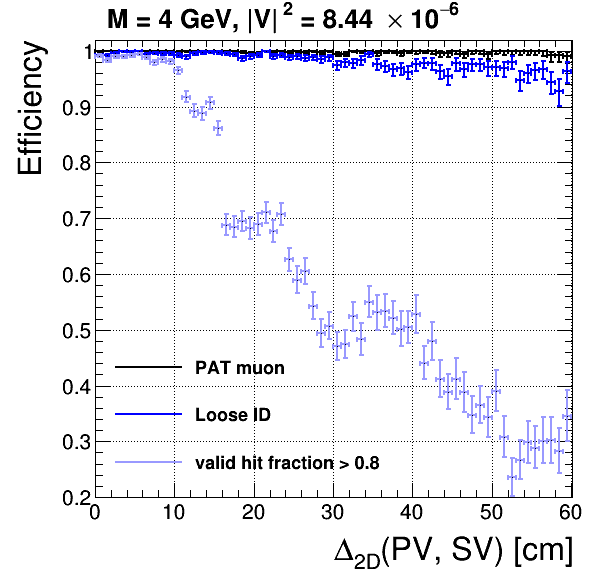
\includegraphics[width=.27\textwidth]{Figures/c6/object/loose_validFraction_M-4_V-0p00290516780927_rho.png}
  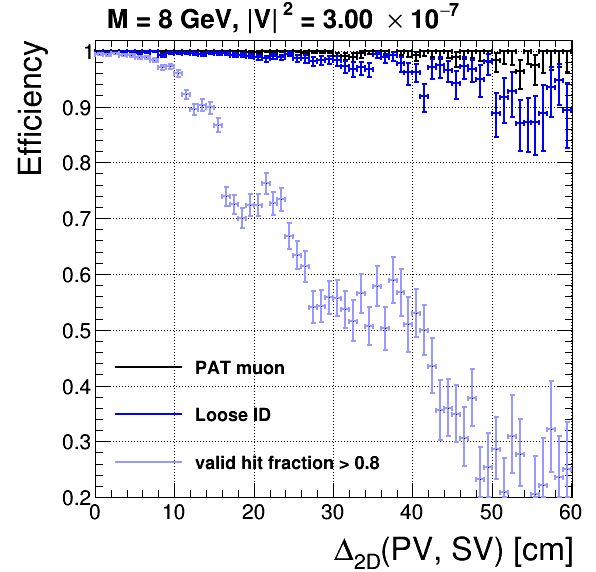
\includegraphics[width=.27\textwidth]{Figures/c6/object/loose_validFraction_M-8_V-0p000547722557505_rho.png}}}\\
 \makebox[\textwidth]{ \subfloat[]{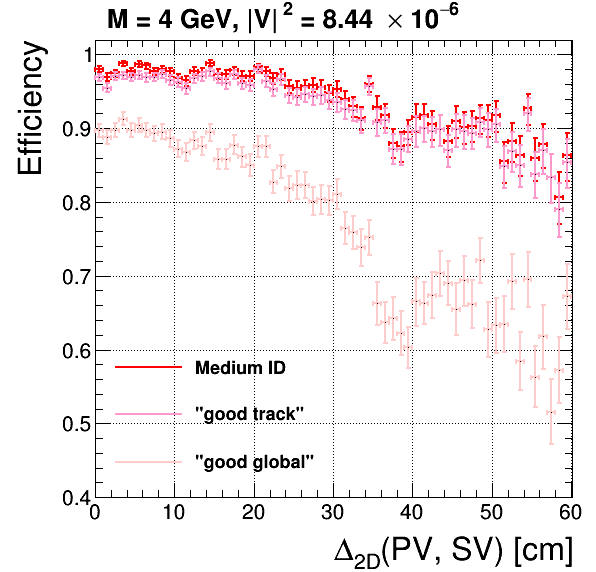
\includegraphics[width=.27\textwidth]{Figures/c6/object/goodTrack_goodGlobal_M-4_V-0p00290516780927_rho.png}
  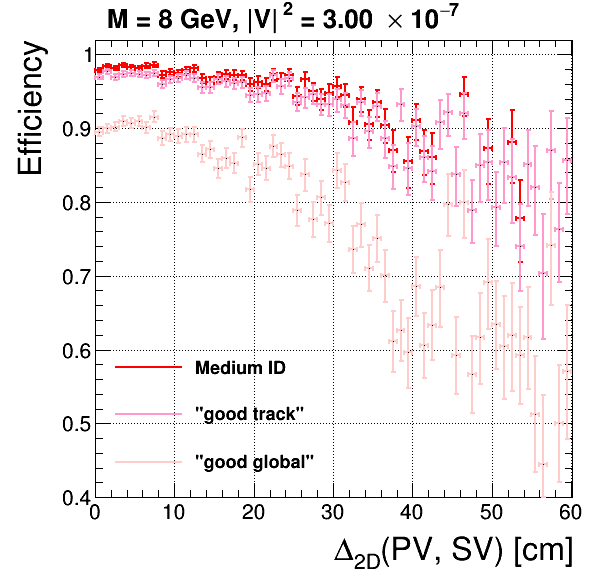
\includegraphics[width=.27\textwidth]{Figures/c6/object/goodTrack_goodGlobal_M-8_V-0p000547722557505_rho.png}}
\subfloat[]{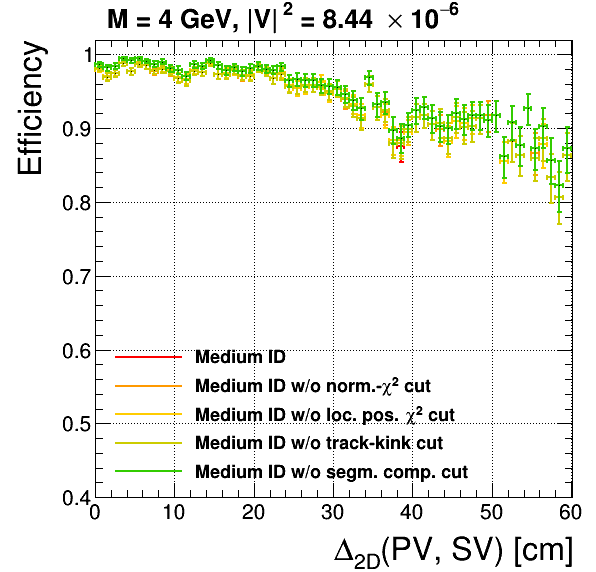
\includegraphics[width=.27\textwidth]{Figures/c6/object/globalTrack_cuts_M-4_V-0p00290516780927_rho.png}
  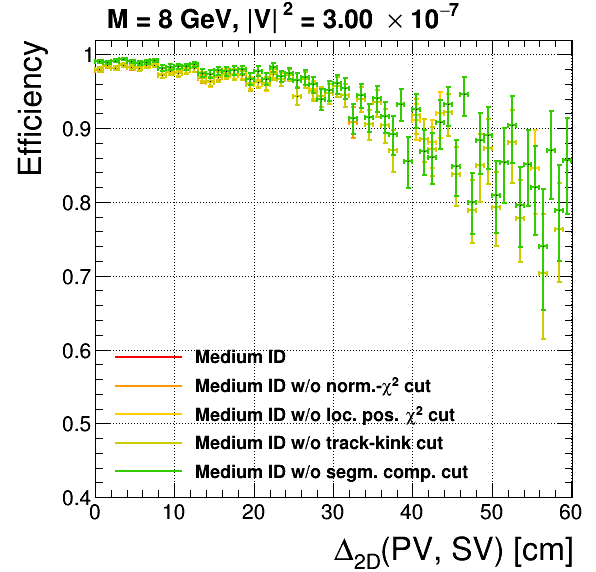
\includegraphics[width=.27\textwidth]{Figures/c6/object/globalTrack_cuts_M-8_V-0p000547722557505_rho.png}}}
  \caption{Efficiency of different Medium-ID selections with respect
    to tracks for \displ
    muons in signal scenarios as a function \Deltwod.}
  \label{fig:modMedium_common}
\end{figure}

\textbf{Jet selection and $\boldsymbol{p_{T}^{miss}}$}: the same selection as described in Sec.~\ref{sec:jet} is deployed.


\section{Analysis strategy}\label{sec:llanalisi}
Signal events are
characterized by the presence of a prompt lepton (in the following
often referred to as \lone, or ``\lept from \PW'' in some figures),
two \displ leptons (\ltwo and \lthree, or
``\lept from \hnl'' and ``\lept from $\hnl\to\PW^\ast$'' in some
figures), and a neutrino, see Fig.~\ref{fig:c6llsketch}.

\begin{figure}[h]
\centering
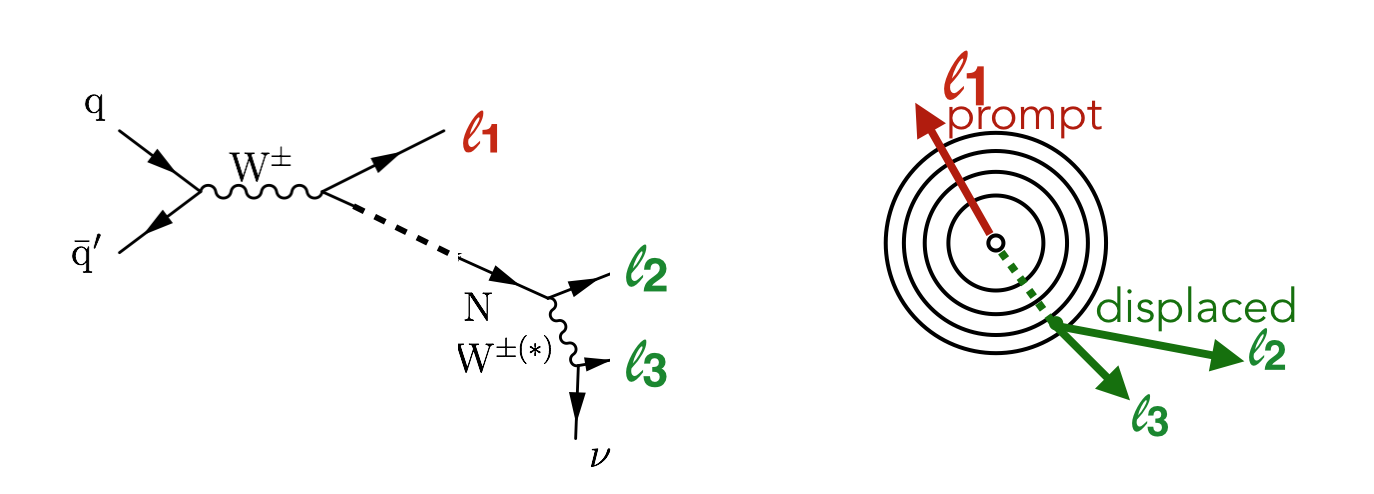
\includegraphics[width=0.85\textwidth]{Figures/c6/llsketch}
\caption{Diagram for the production of a long-lived HNL (left) with colors
  underlining the nomenclature adopted in the following
  sections. Prompt lepton often referred to as \lone, or ``\lept from
  \PW'' in some figures, and two \displ leptons (\ltwo and \lthree, or
``\lept from \hnl'' and ``\lept from $\hnl\to\PW^\ast$'' in some
figures. Didactic sketch on the right showing the usual signature with
 \lone back-to-back wrt \ltwo and \lthree which form a SV.}
\label{fig:c6llsketch}
\end{figure}

In the following sections, events are split into  
final states in which \lone and at least one of \ltwo or \lthree are
electrons (\eex) or muons (\mmx).
Events with \eex final states are sensitive to the \mixpare parameter,
while \mmx events are sensitive to the \mixparm parameter.

Figure~\ref{fig:llfeatures} illustrates some
kinematic properties of the leptons in signal events, both at the
generator and reconstruction levels.
Given the low HNL masses considered in this analysis (\mhnl < 20\GeV),
\lone has the typical \pt spectrum expected for \PW decays, with a
Jacobian peak around 40\GeV,
while \ltwo and \lthree have very soft \pt spectra (Fig.~\ref{fig:llfeatures}(A)), invariant mass smaller than \mhnl (Fig.~\ref{fig:llfeatures}(B)), and a small opening angle
(Fig.~\ref{fig:llfeatures}(C)).
In the absence of significant hadronic activity, \lone and \hnl are
typically separated by a large azimuthal angle (Fig.~\ref{fig:llfeatures}(D)).
These features, along with the possible displacement of \ltwo and
\lthree, can be used to identify the two leptons coming from the HNL
decay.

\begin{figure}[h]
\noindent
\makebox[\textwidth]{  \subfloat[]{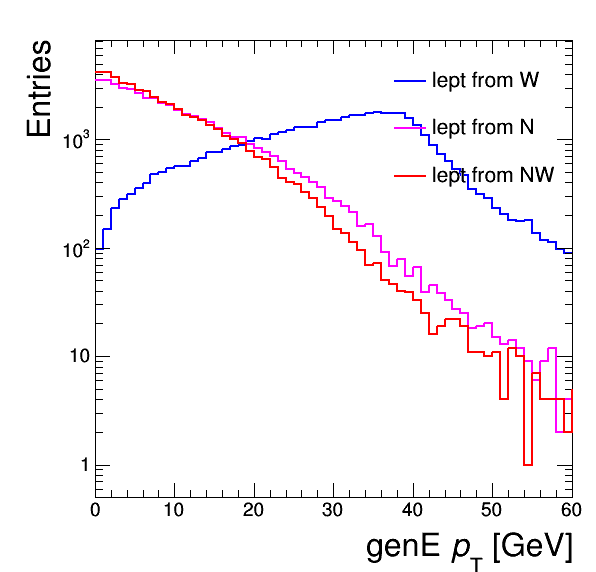
\includegraphics[width=.27\textwidth]{Figures/c6/selection/genE_vs_pt_sortby_prov_m4.png}
  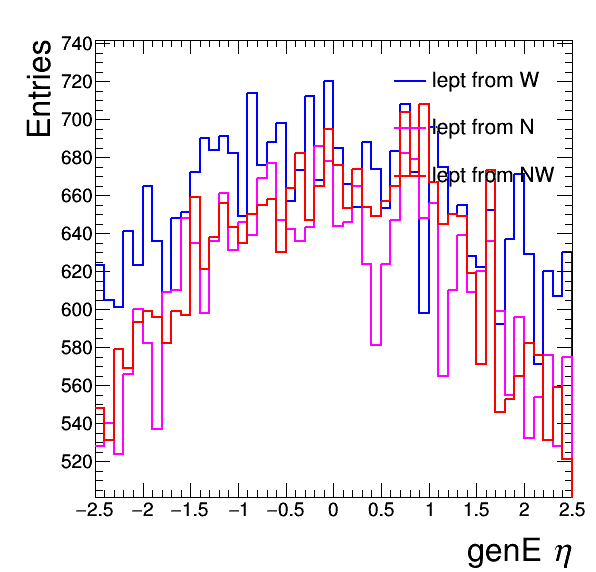
\includegraphics[width=.27\textwidth]{Figures/c6/selection/genE_vs_eta_sortby_prov_m4.png}}
  \subfloat[]{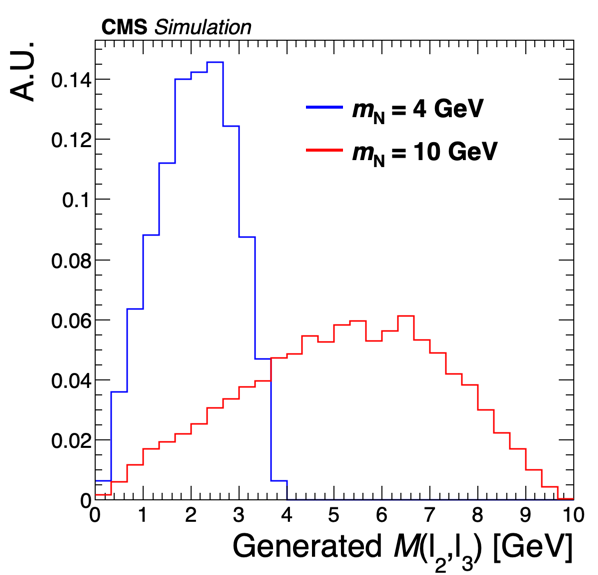
\includegraphics[width=.27\textwidth]{Figures/c6/selection/l2l3_mass_gen.png}
  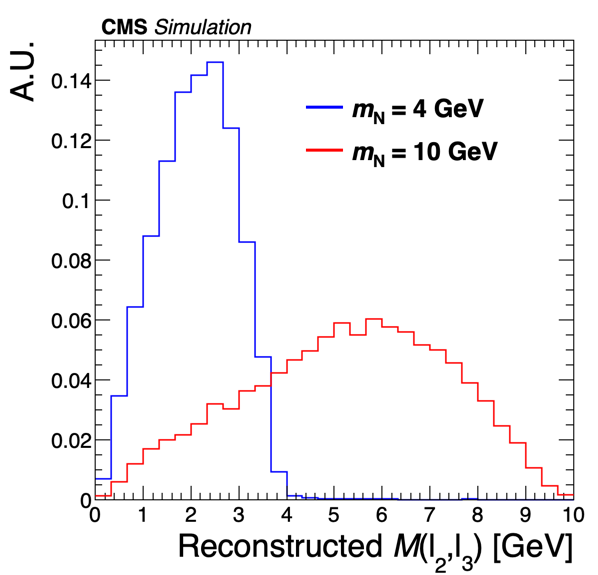
\includegraphics[width=.27\textwidth]{Figures/c6/selection/l2l3_mass_rec.png}}}\\
 \makebox[\textwidth]{ \subfloat[]{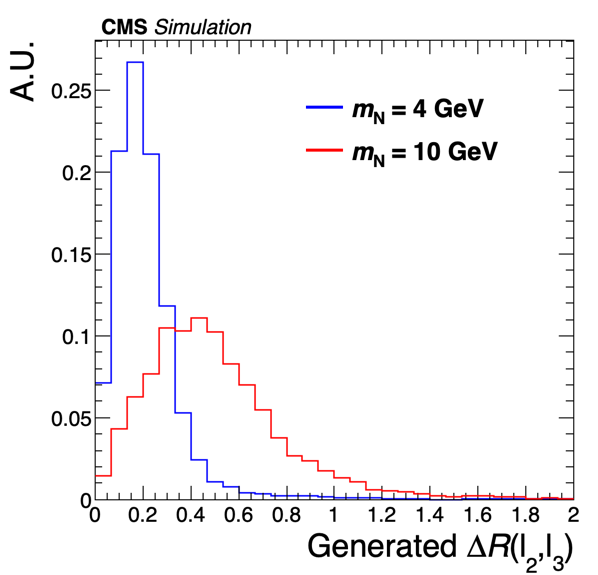
\includegraphics[width=.27\textwidth]{Figures/c6/selection/l2l3_dR_gen.png}
  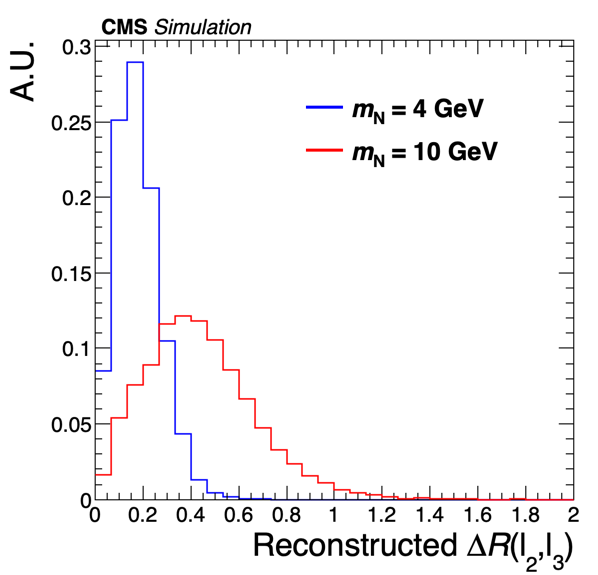
\includegraphics[width=.27\textwidth]{Figures/c6/selection/l2l3_dR_rec.png}}
\subfloat[]{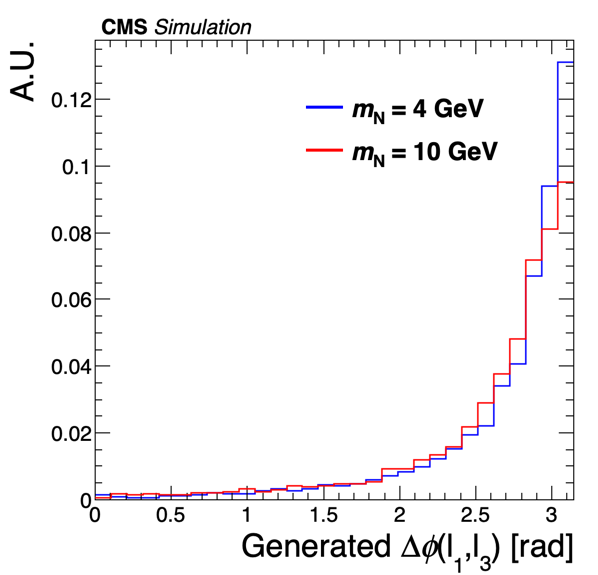
\includegraphics[width=.27\textwidth]{Figures/c6/selection/l1l3_dPhi_gen.png}
  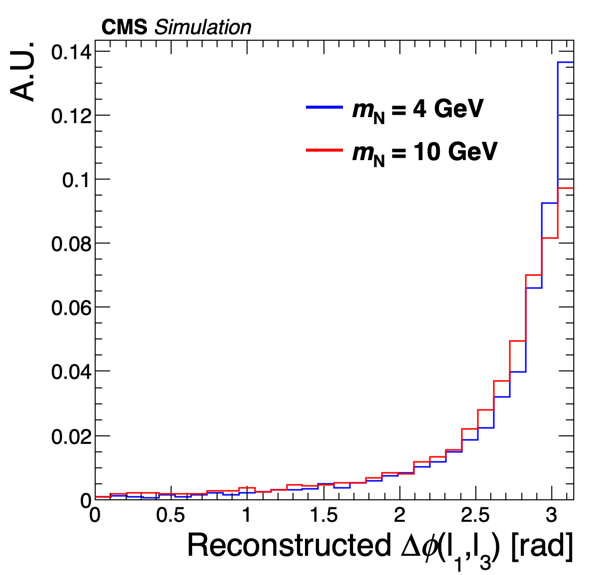
\includegraphics[width=.27\textwidth]{Figures/c6/selection/l1l3_dPhi_rec.png}}}
  \caption{A) Generated lepton \pt (left) and \sigeta (right), separately
    for \lone (``from \PW''), \ltwo (``from \hnl''), and \lthree
    (``from $\hnl\PW$''), produced in the decay of a HNL of mass
    $\mhnl=4\GeV$ and $\mixpar=10^{-4}$.\\
B) Invariant mass of \ltwo
    and \lthree 
    at generator level (left) and at reconstructed level (right), for
    a HNL of mass $\mhnl=4\GeV$ or 10\GeV, and $\mixpar=10^{-4}$.
    Events in these distributions are pre-selected requiring the
    presence of three reconstructed leptons, as defined in
    Tables~\ref{tab:electronSelection} and \ref{tab:muonSelection},
    with the prompt lepton firing a single-lepton trigger, as per
    Table~\ref{tab:sgnlTriggers}.
C) \DR\ between \ltwo 
    and \lthree.
D) \Dphi between \lone
    and \lthree.}
  \label{fig:llfeatures}
\end{figure}

\subsection{HNL candidate selection}
As shown in Tables~\ref{tab:electronSelection} and
\ref{tab:muonSelection},
the displacement of \ltwo and \lthree is requested by imposing a
minimum \absdxy cut of 0.1~mm to the reconstructed leptons.
Given the rapid variation of the \hnl displacement with \mhnl and
\mixpar, this preliminary displacement requirement must be rather
mild, and does not resolve completely possible ambiguities between
prompt and \displ reconstructed leptons.

Other than the two leptons from the HNL decay, additional
leptons---real or misidentified---may satisfy the \absdxy requirements
and pass the \displ-lepton selection. In this case, criteria must
be put in place to resolve the ambiguities and correctly identify the
two leptons from the HNL decay.
To this purpose, variables such as the invariant mass of \ltwo and
\lthree, \mtwol, and the \DR\ separation between \ltwo and \lthree, \DRtwol, are found to be
effective, and with similar performance.
Therefore, the three leptons from HNL decay are identified as follows.
Among all the leptons that pass the prompt selection of
Tables~\ref{tab:electronSelection} and \ref{tab:muonSelection}, the one
with highest \pt is chosen as \lone and it is not considered anymore for the selection of \ltwo and \lthree.
Among all the selected \displ leptons, the two leptons of any
flavor with the lowest invariant mass and opposite charge are selected
as \ltwo and \lthree,
($\Pe^\pm\Pe^\mp$, $\Pe^\pm\PGm^\mp$, $\PGm^\pm\PGm^\mp$).
If there is no opposite-charge \displ leptons pair, the
event is rejected. 

This reduces background processes with
mis-identified leptons, while retaining almost full efficiency for the
signal. In the following, we will label \ltwo (\lthree) the lepton in
the pair with higher (lower) \pt.

This selection strategy correctly identifies the one prompt and two
\displ leptons in more than 99\% of signal events (99.9\% of
signal events that pass the full analysis selection, described in
Section~\ref{sec:baselinesel}).

\subsection{Secondary vertex fit and lepton extrapolation}

Once \ltwo and \lthree have been identified, we can reconstruct their
common vertex of origin, \ie the decay vertex of the HNL. This is done
by fitting the two tracks to a common point with a Kalman-filter
approach~\cite{kvfTwiki},
using the
\texttt{KalmanVertexFitter} class implemented in \texttt{CMSSW} framework.
The class returns the least-$\chi^2$ estimator of the two-track vertex
position and covariance matrix, along with the $\chi^2$ of the fit, as
an indicator of its goodness.
Figure~\ref{fig:svPulls} shows the pulls of the distance of the fitted
secondary vertex (SV) from the PV of the interaction, in three
dimensions (denoted as $R$ in the left figure) or projected on the
transverse plane (denoted as $\rho$ in the right figure). The pulls
are computed as the difference between the measured distance ($R$ or
$\rho$) and its true value from simulation, divided by the uncertainty
on the measured value. A standard deviation of about 1.2 is found from
a Gaussian fit to the pull distributions, revealing a slight
underestimation of the uncertainties.
\begin{figure}[h!]
  \centering
  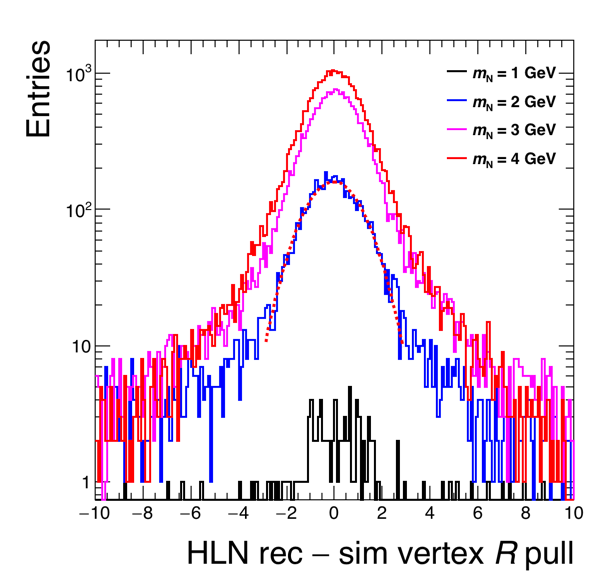
\includegraphics[width=.34\textwidth]{Figures/c6/selection/leptons_fromN_fromNW_vtx_r_pull.png}
  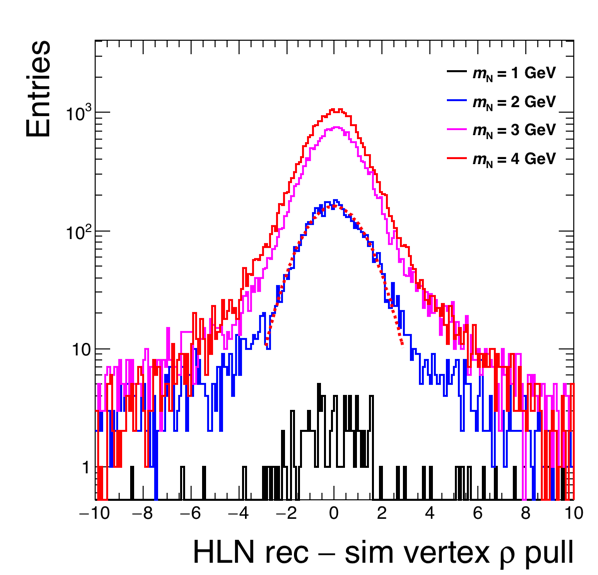
\includegraphics[width=.34\textwidth]{Figures/c6/selection/leptons_fromN_fromNW_vtx_rho_pull.png}
  \caption{Pull distributions of the three-dimensional (left) and
    transverse (right) distance of the fitted secondary vertex from
    the PV of the interaction, for HNL masses from 1 to 4\GeV,
    all with $\mixpar=10^{-4}$. The red curve overlaid to the blue
    histogram shows a Gaussian fit to the core of the \mhnl= 2\GeV
    distribution.}
  \label{fig:svPulls}
\end{figure}
Figure~\ref{fig:svResidVsRho_all} shows the residuals of the
transverse PV--SV distance $\rho$ with respect to the true generated
value, $\Delta\rho(\mathrm{gen,rec})$ (left), and the relative residuals
$\Delta\rho(\mathrm{gen,rec})/\rho(\mathrm{gen})$ (right), as a
function of the true $\rho$, for signal events satisfying the final
signal selection that will be described in
Section~\ref{sec:baselinesel} and summarized in
Table~\ref{tab:baselinesel}. No significant biases are observed and
the tails are small: the fraction of events with
$\Delta\rho(\mathrm{gen,rec})/\rho(\mathrm{gen})$ larger than
10\%---indicated by the dashed horizontal lines in
Fig.~\ref{fig:svResidVsRho_all} (right)---is about 2.6\% for
transverse displacement $\rho$ < 0.5cm, and less than 1\% for larger
displacements.
Figure~\ref{fig:svResidVsRho_all}(A-B-C) shows the same
$\Delta\rho(\mathrm{gen,rec})$ distribution in different dilepton \pt
ranges for all flavor combinations: 15--20\GeV (A), 20--30\GeV
(B), and $>30\GeV$ (C).
Figure~\ref{fig:svResidVsRho_all}(D) shows the
$\Delta\rho(\mathrm{gen,rec})$ profiles for different flavor final
states ($\Pe\Pe$, $\Pe\PGm$, $\PGm\PGm$) for any dilepton transverse
momentum.
No large biases are observed at any dilepton \pt, nor for
any dilepton flavor.
\begin{figure}[t]
  \noindent
\makebox[\textwidth]{ 
  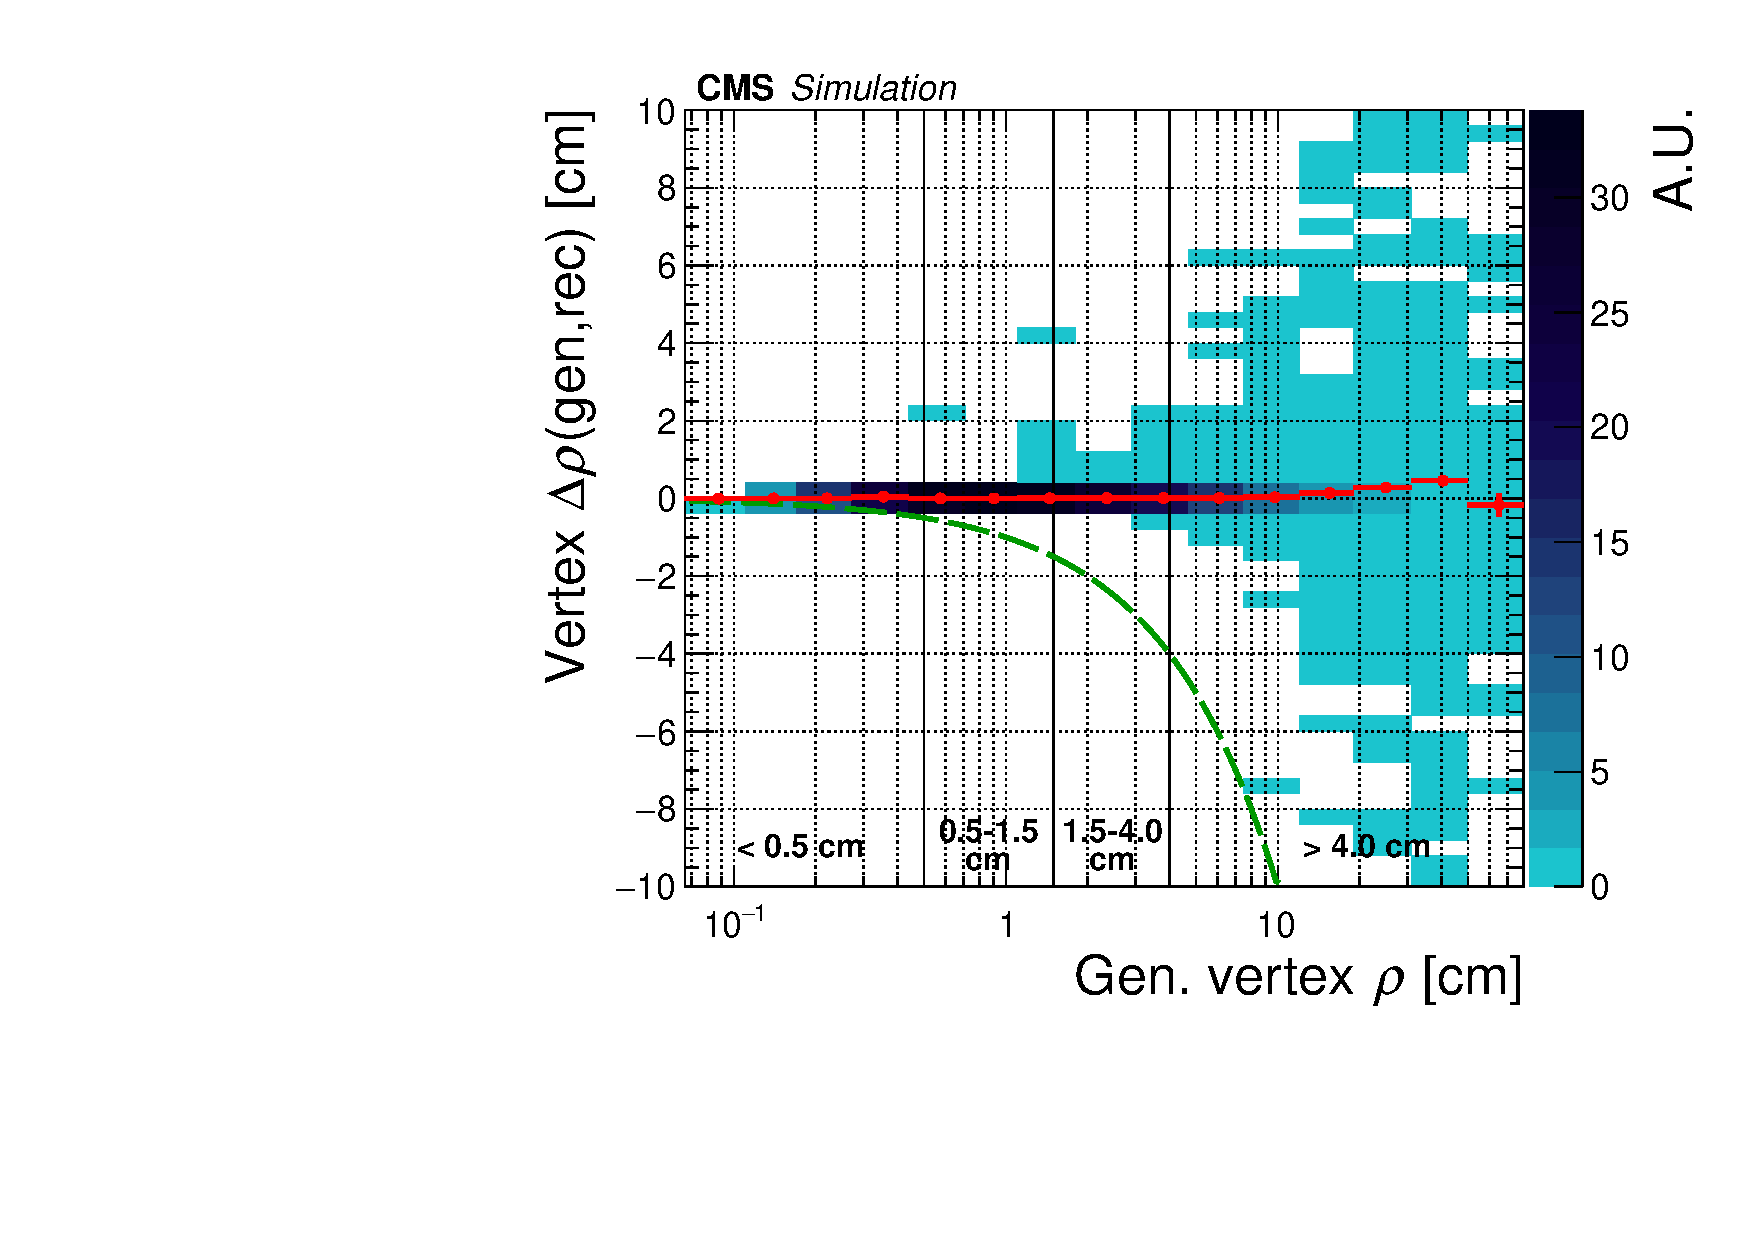
\includegraphics[width=.38\textwidth]{Figures/c6/selection/genvtx_recvtx_Drho_vs_rho_afterSel_zoom.pdf}
  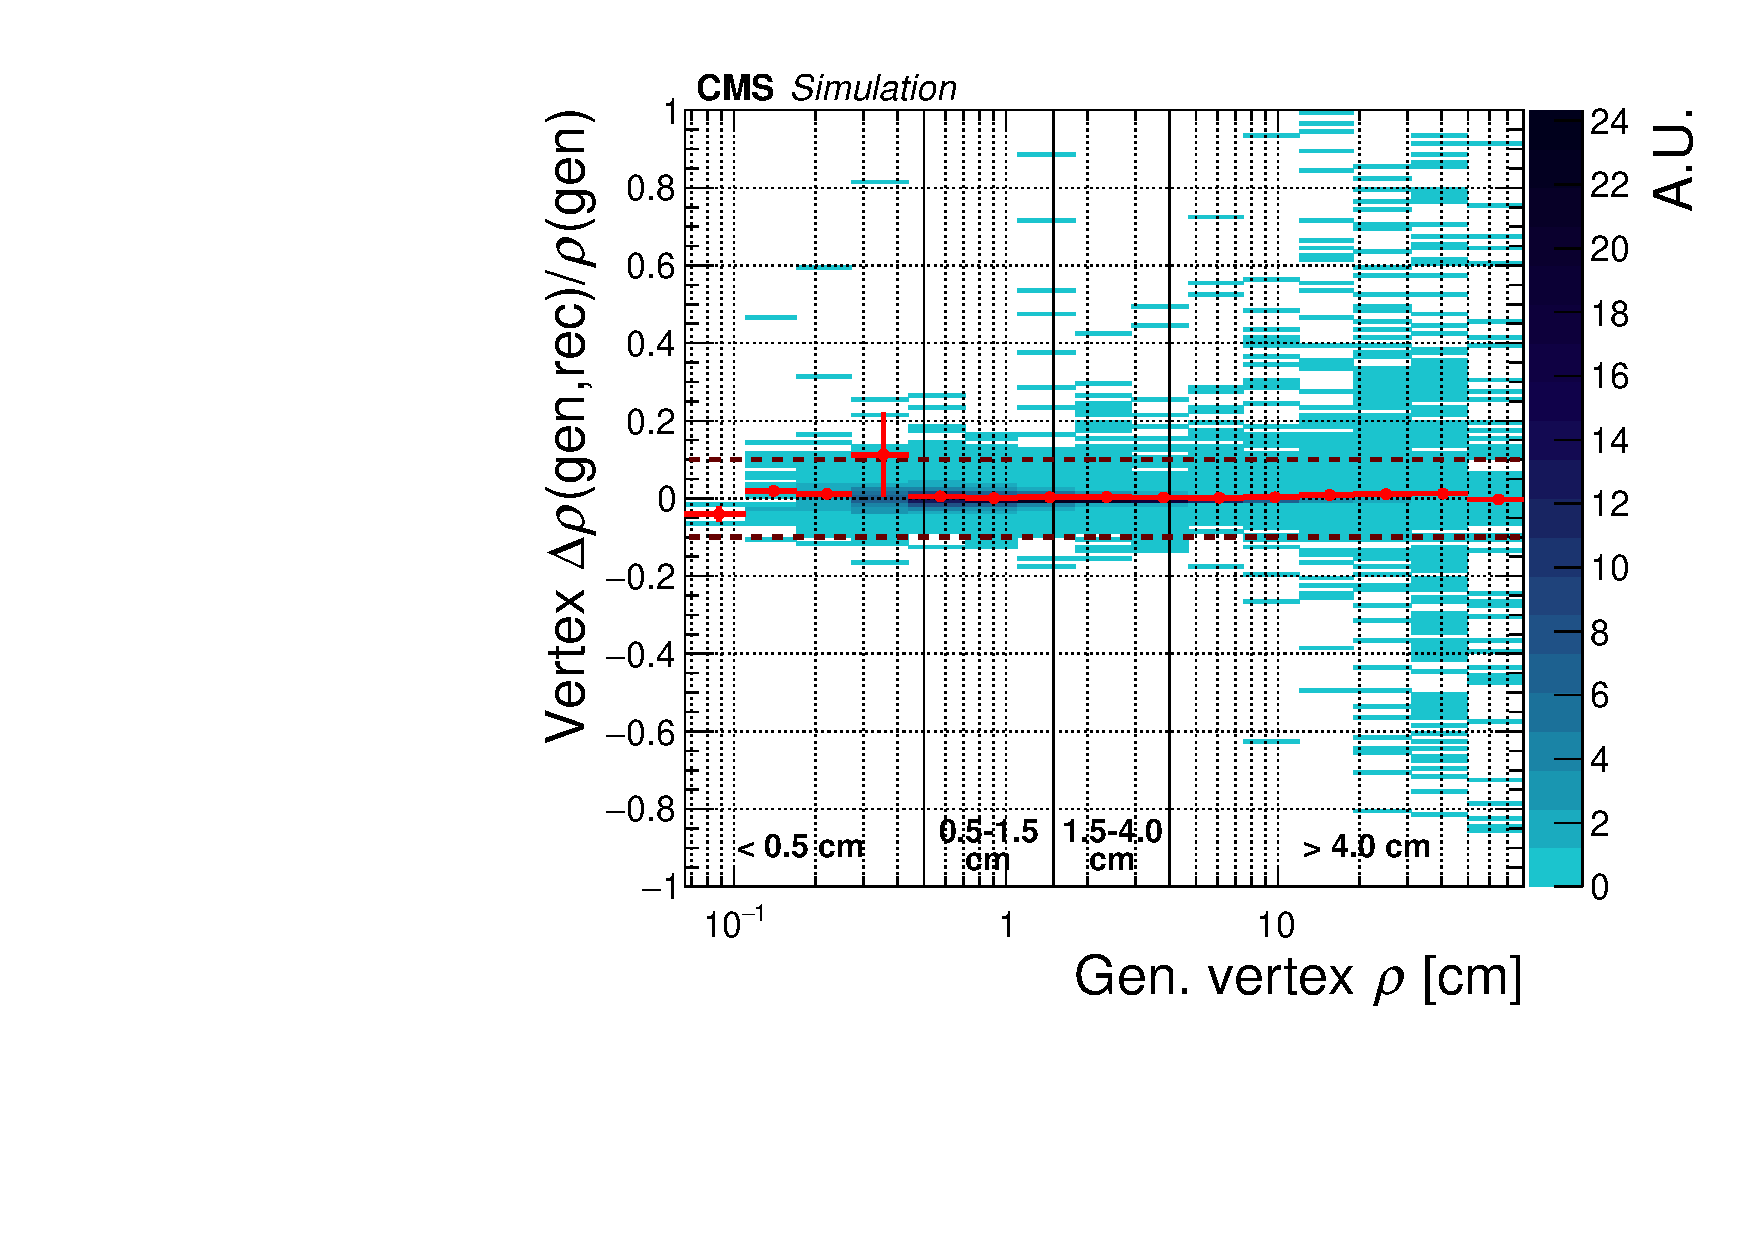
\includegraphics[width=.38\textwidth]{Figures/c6/selection/genvtx_recvtx_RelDrho_vs_rho_afterSel_zoom.pdf}}\\
\makebox[\textwidth]{  \subfloat[]{
  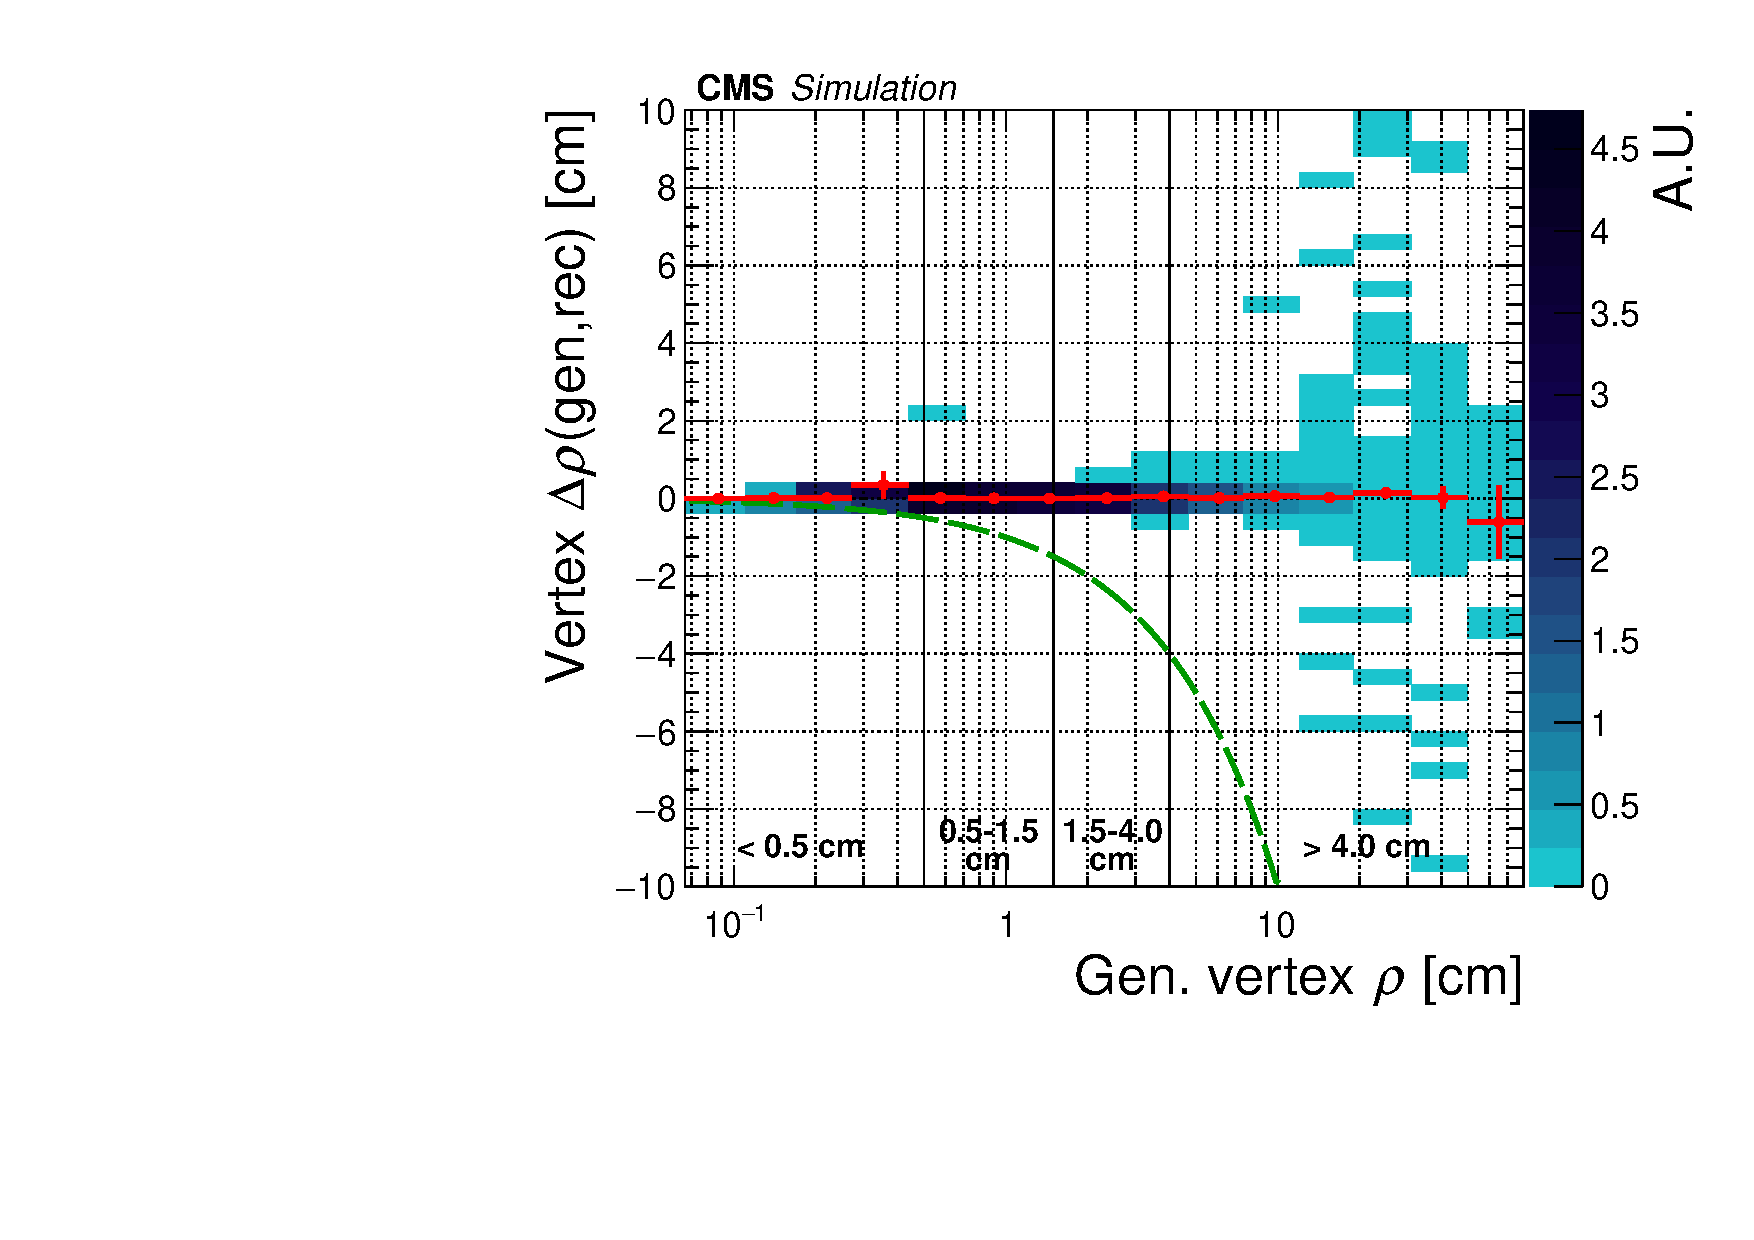
\includegraphics[width=.38\textwidth]{Figures/c6/selection/pt15to20_genvtx_recvtx_Drho_vs_rho_afterSel_zoom.pdf}}
  \subfloat[]{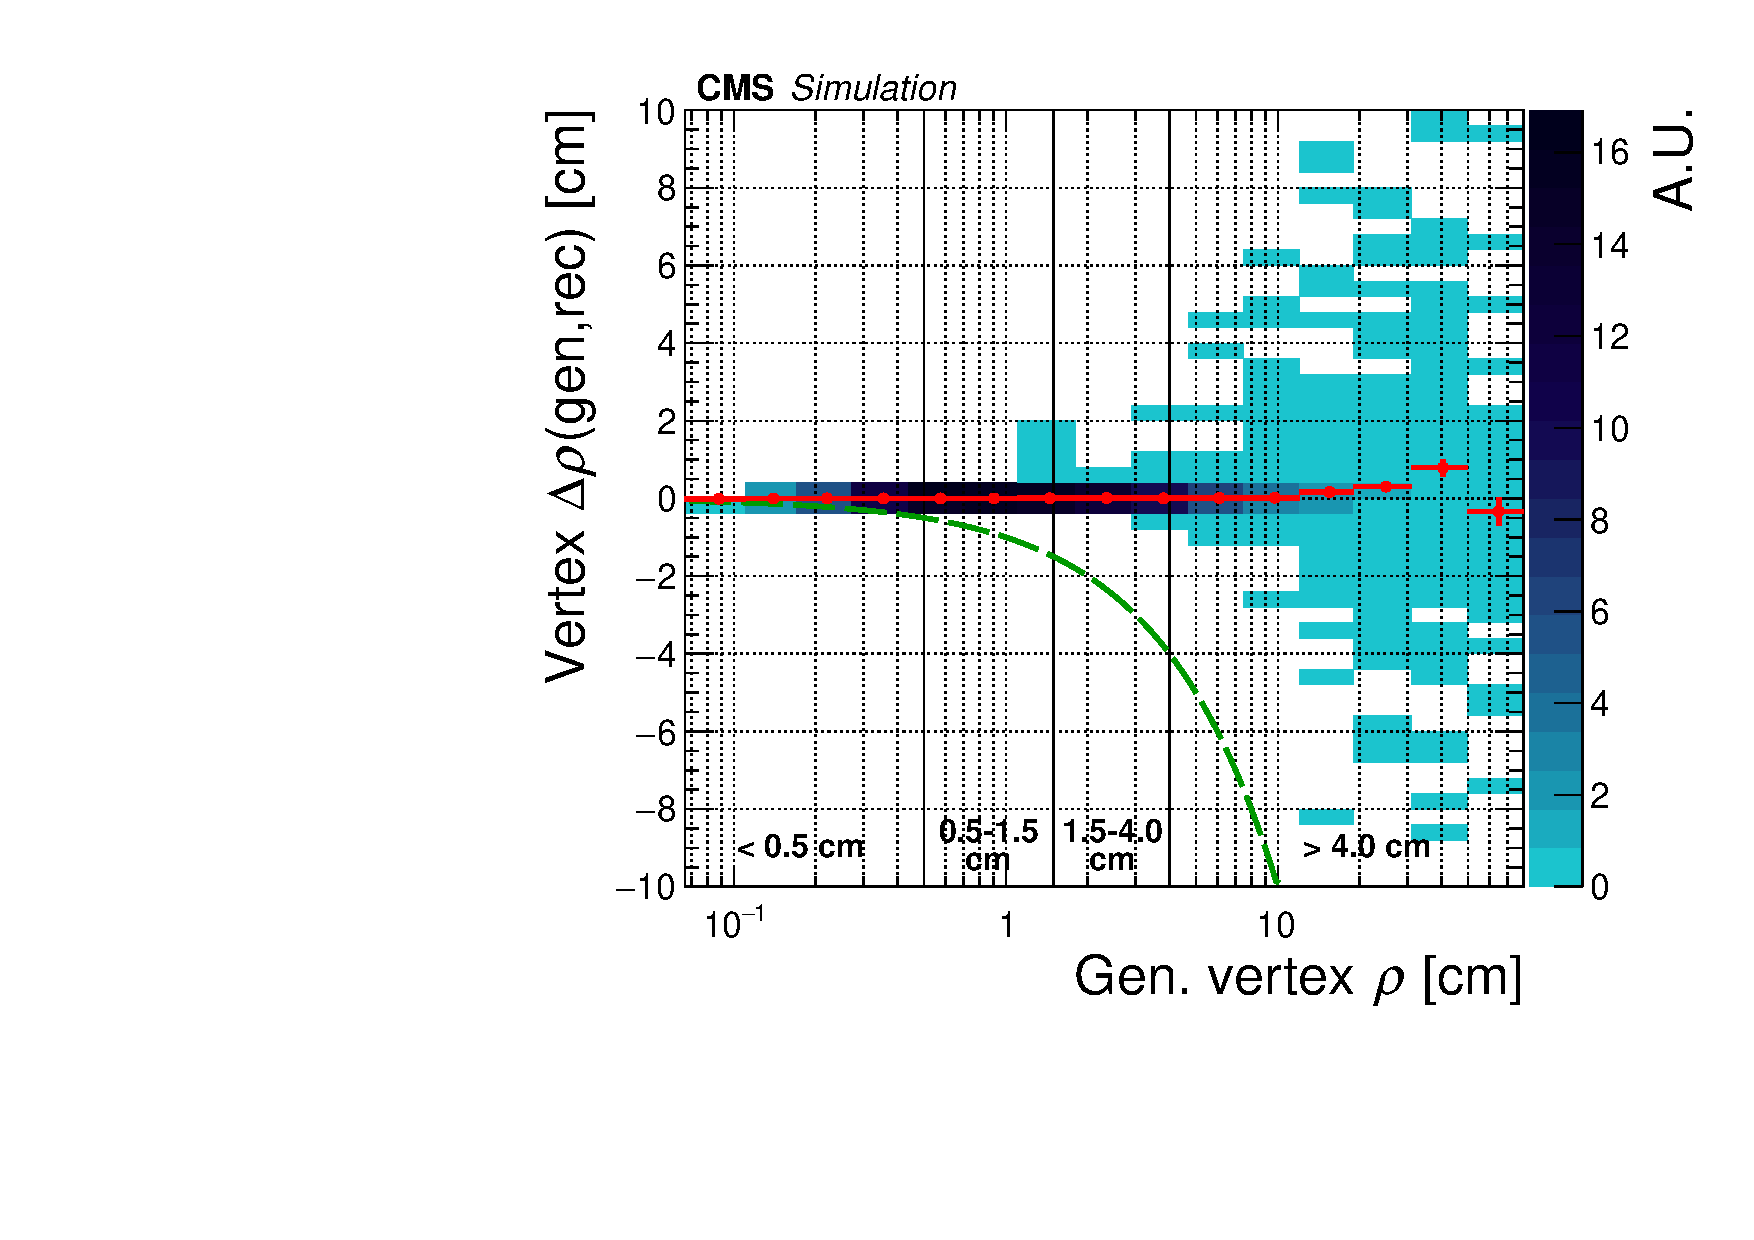
\includegraphics[width=.38\textwidth]{Figures/c6/selection/pt20to30_genvtx_recvtx_Drho_vs_rho_afterSel_zoom.pdf}}}\\
\makebox[\textwidth]{  \subfloat[]{
  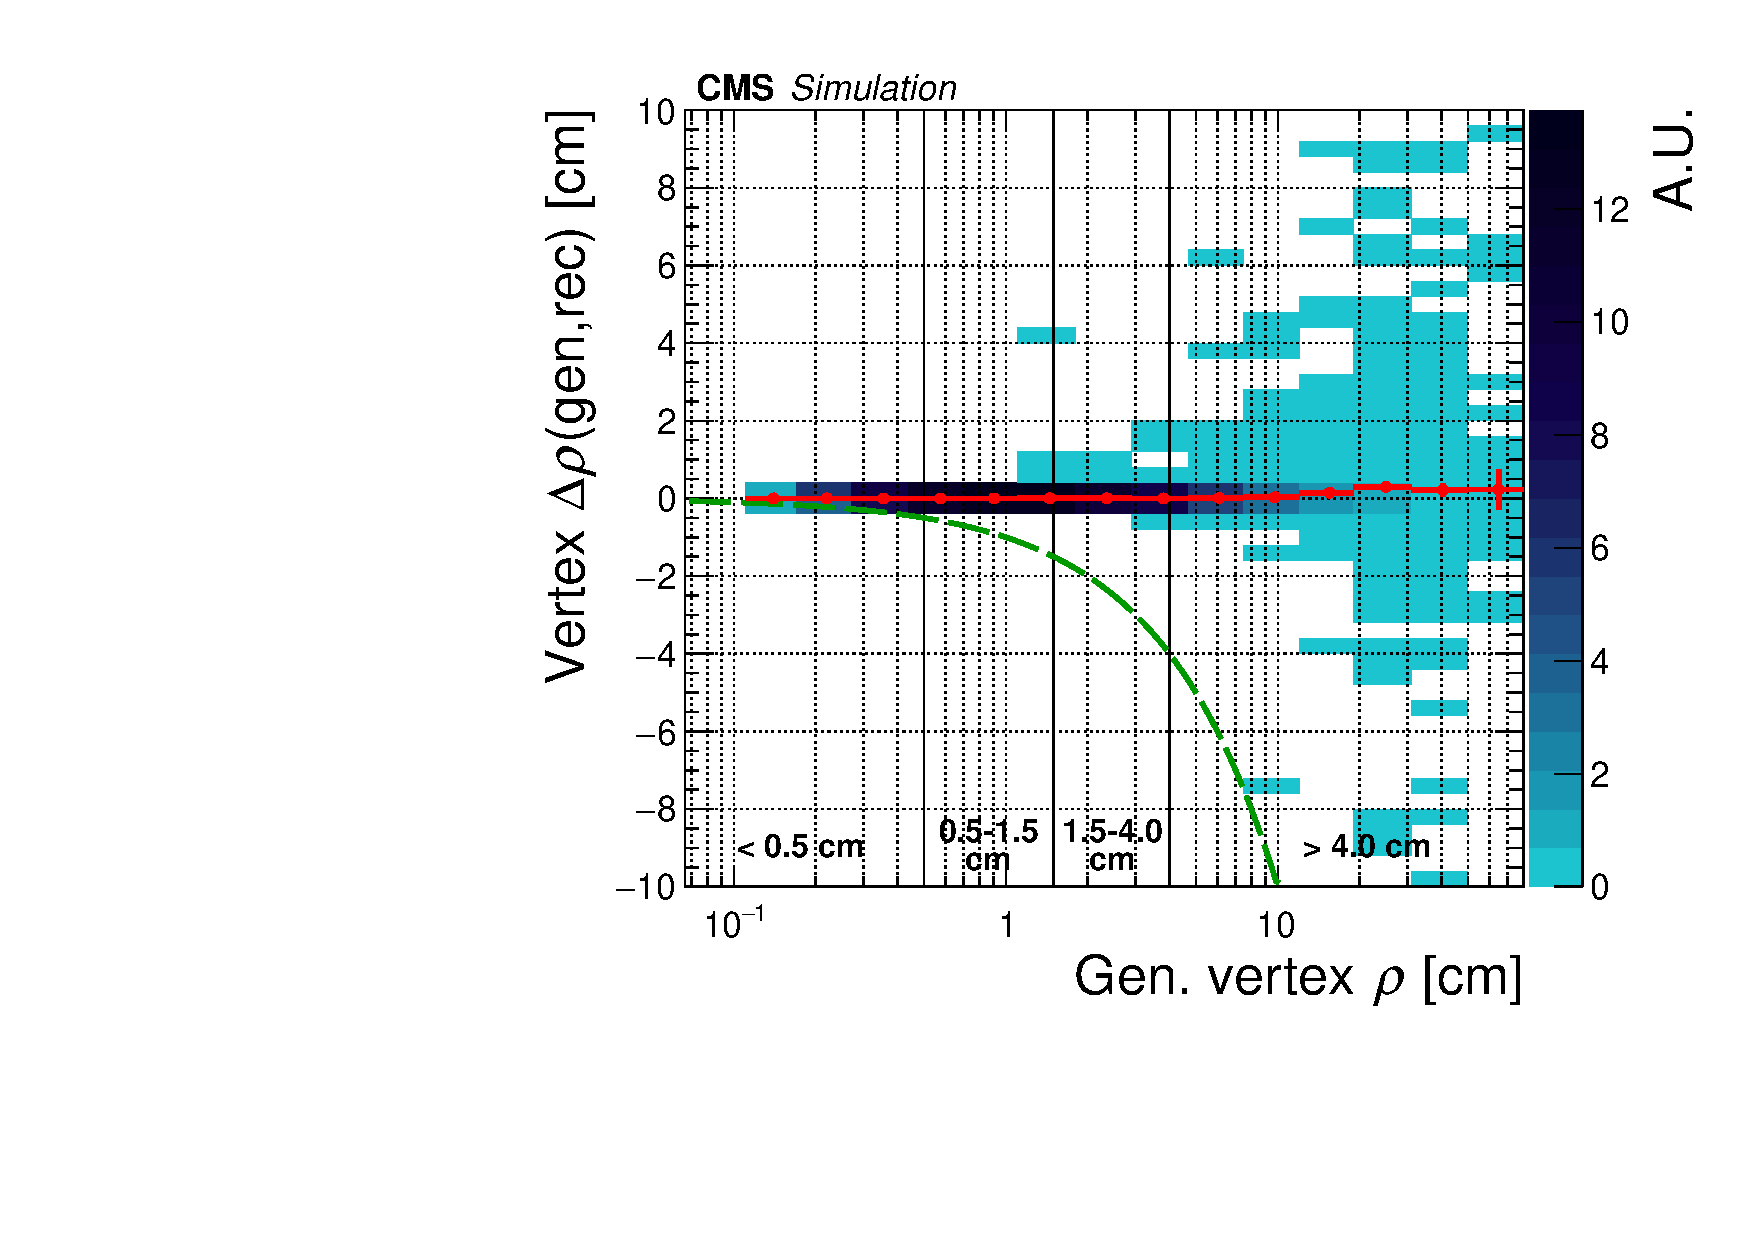
\includegraphics[width=.38\textwidth]{Figures/c6/selection/pt30toInf_genvtx_recvtx_Drho_vs_rho_afterSel_zoom.pdf}}\hspace{7mm}
  \subfloat[]{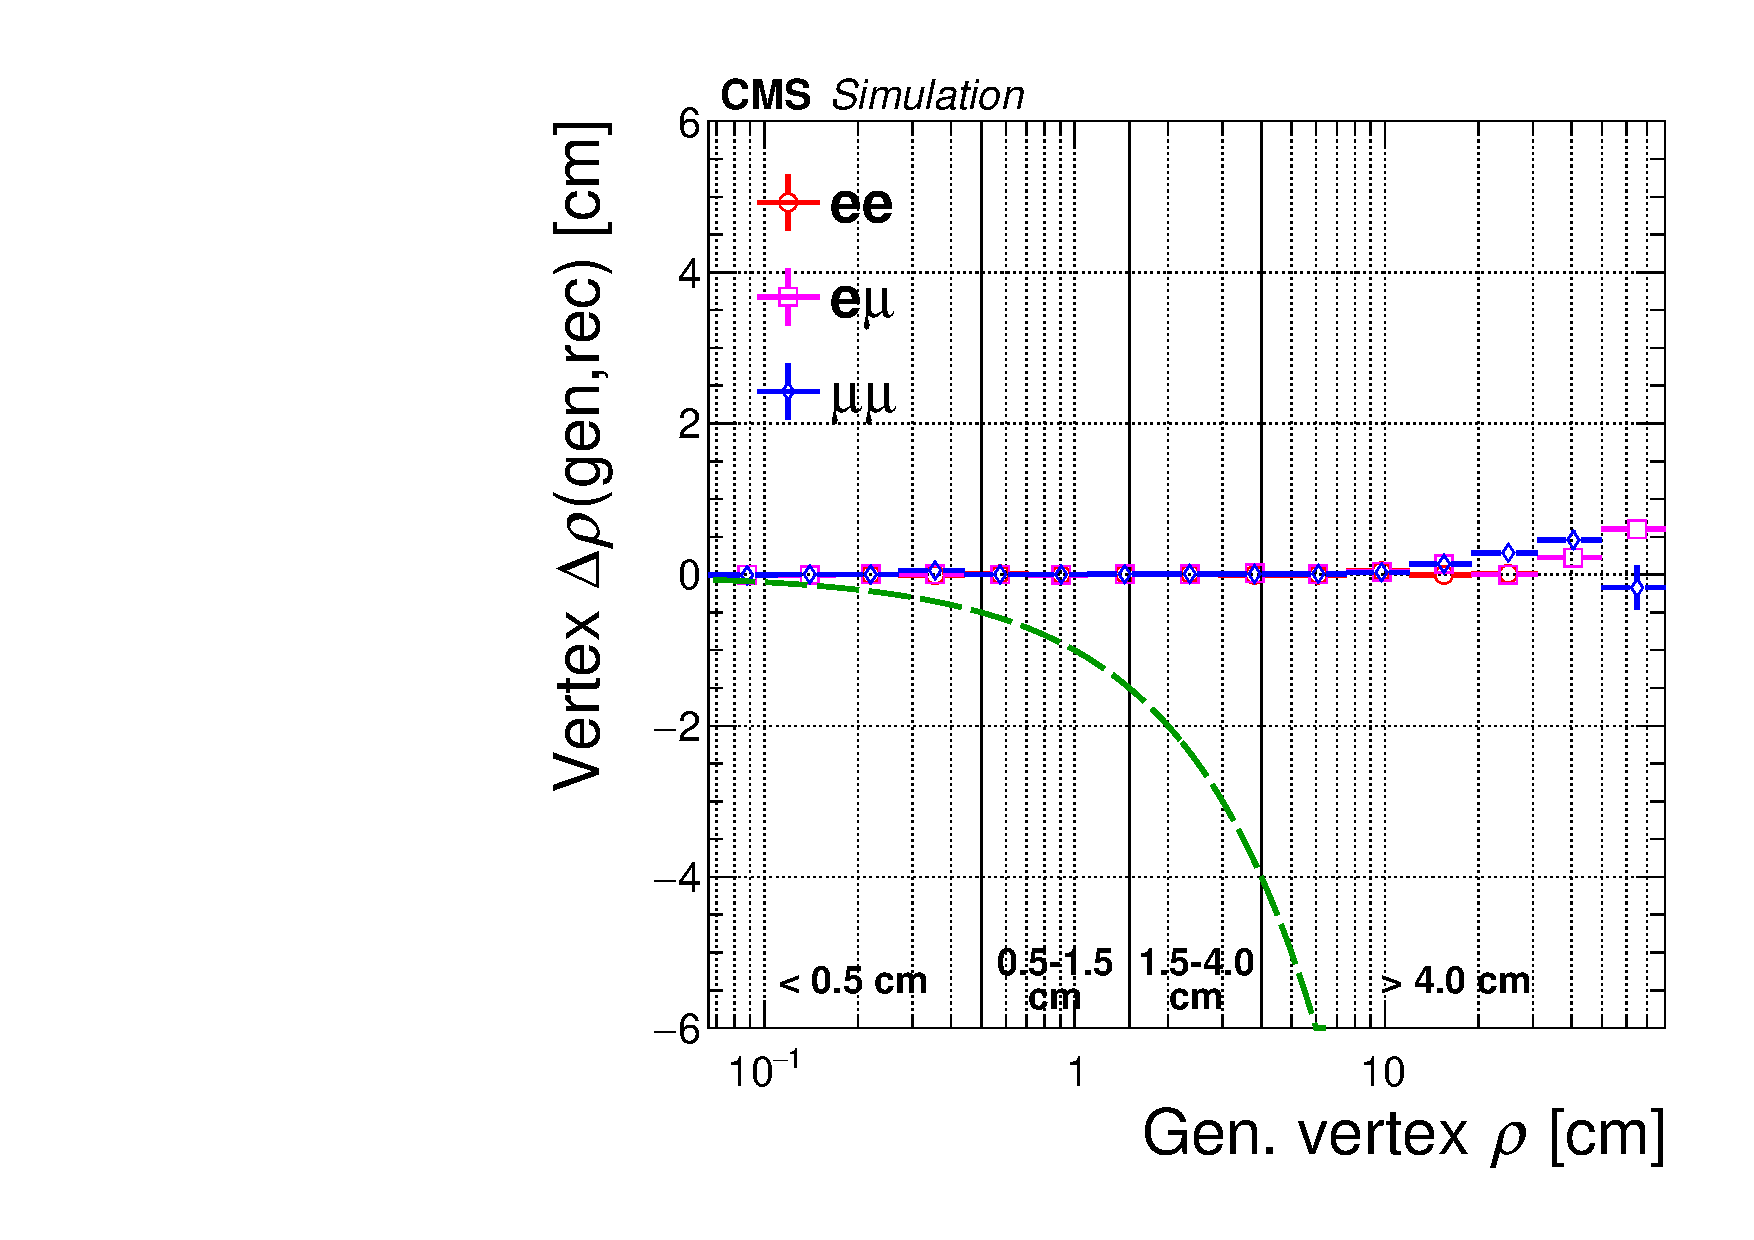
\includegraphics[width=.32\textwidth]{Figures/c6/selection/finalstates_genvtx_recvtx_Drho_vs_rho_afterSel_zoom.pdf}}}
  \caption{A) Residuals (left) and relative residuals (right) of the
    transverse distance $\rho$ between the fitted secondary vertex and
    the PV of the interaction, as a function of the true $\rho$ value
    from simulation. All lepton flavors are included.
    The red graph shows the mean value of the
    residuals in each $\rho$ bin and the uncertainty on the mean
    value. The dashed green line in the left plot indicates the
    distance between the generated primary and secondary vertices: any
    reconstructed vertex below this line would lie in the ``wrong''
    emisphere, opposite to the direction of flight of the HNL.
    The horizontal dashed lines in the right plot delimit the region
    where $\Delta\rho(\mathrm{gen,rec})$ is less than 10\% of
    $\rho(\mathrm{gen})$. 
    The three plots A-B-C correspond to
    different values of the dilepton \pt (thus different average
    opening angles of the two leptons), for all lepton flavors:
    15--20\GeV (A), 20--30\GeV (B), and $>$30\GeV
    (C). The bottom right plot shows separate profiles for
    the three flavor final states ($\Pe\Pe$, $\Pe\PGm$, $\PGm\PGm$),
    for any dilepton \pt.
    To have enough statistics in all the $\rho$ bins, a combination of
    all the signal samples (2018 only) is used.}
  \label{fig:svResidVsRho_all}
\end{figure}
The fitted SV estimates the production vertex of \ltwo and \lthree.

\clearpage
\subsection{Event kinematics and baseline selection}
\label{sec:llbaselinesel}

Starting from all the events with one prompt lepton and two \displ
leptons forming a SV (following the definitions and strategies
described above), the kinematic properties and particle content of
typical HNL signal events are used to suppress the SM backgrounds:
most importantly, processes with one or two fake leptons,
such as top-quark production
(\ttbar, $t\PW$, $t$- and $s$-channel single top),
\(\PZ/\PGg^{\ast}+\mathrm{jets}\), and \(\PW+\mathrm{jets}\);
and processes with a real photon that converts into lepton
pairs---mostly electrons---in the detector material, such as
$\PW\PGg$ and $\PZ\PGg$. \\

The baseline selection includes the following requirements, summarized
in Table~\ref{tab:baselinesel}. Please
consider Fig.~\ref{fig:c6llsketch} as reference.

\begin{table}[h]
  \centering
  \caption{\label{tab:baselinesel} Baseline selection requirements
    applied to all data sets.}
  \begin{tabular}{l|l}
    \hline
    Variable     & Requirement       \\
    \hline
    \hline
       \DRtwol      & $<1$              \\
    \minDphi     & $>1$ rad          \\
    \mlll     & $\in [50,80]\GeV$ \\
    N. \PQb jets & $=0$              \\
    \pt (\ltwo $+$ \lthree) & $> 15 \GeV$              \\
    \costheta    & $>0.99$            \\
    SV probability & $> 0.001$              \\
    $\Delta (PV-SV)_{2D} / \sigma$& $>20$              \\ 
    resonance vetoes & applied      \\
    \hline
    \hline
  \end{tabular}
\end{table}

As explained above, \ltwo and \lthree are expected to have small
opening angle, given the small mass and relatively large momentum of
the HNL. As can be seen in
Figures.~\ref{fig:selection_electrons},~\ref{fig:selection_muons} (top-left),
the variable \DRtwol discriminates the signal from all background
processes. To retain high signal efficiency, we select events with
$\boldsymbol{\DRtwol<1}$.
\vspace{2mm}

In the absence of energetic jets in signal events, \lone is expected
to recoil at a large angle in the transverse plane from the HNL, and
thus from \ltwo and \lthree. Since both $\Dphi(\lone,\ltwo)$ and
$\Dphi(\lone,\lthree)$ are large and close in value (which may not be
true for other processes with two uncorrelated nonprompt leptons), we
apply a cut on the smaller of the two angles,
$\boldsymbol{\minDphi>1\,\mathrm{rad}}$ (see Figures.~\ref{fig:selection_electrons},~\ref{fig:selection_muons} (top-center)). 
\vspace{2mm}

The invariant mass of the three charged leptons \mlll, \mthreel, is limited
by the mass of the on-shell \PW boson. Given the relatively low
momentum carried away by the neutrino, \mlll tends to peak just
below the \PW mass, with a steep fall above 80\GeV and a larger tail
at lower masses (see Figures.~\ref{fig:selection_electrons},~\ref{fig:selection_muons} (top-center)). We select
events with $\boldsymbol{\mlll}$ values \textbf{between 50 and 80\GeV}. This requirement
proves particularly effective against the \Zgs background, where the
photon radiated by one of the leptons from the \PZ decay undergoes an
asymmetric conversion: one of the leptons receives most of the \PGg
momentum, while the other is too soft to be detected or
identified. This explains the peak at about 91\GeV in the \mthreel
spectrum. 
\vspace{2mm}

Events with a \PQb jet (see Section~\ref{sec:object}) with \pt greater
than 25\GeV are rejected, in order to substantially reduce the
background from the top processes.
Figures.~\ref{fig:selection_electrons},~\ref{fig:selection_muons} (top-right) show the number of \PQb jets with \pt greater than 25\GeV.
\vspace{2mm}

The vector sum of the momenta of \ltwo, \lthree, and the neutrino
corresponds to the momentum of the HNL, and points back exactly to the
PV. Unfortunately the total momentum of the neutrino is unknwon, and
its transverse momentum, estimated by \ptmiss, has limited resolution.
The decay products of the HNL, however, are emitted at small opening
angles with respect to the HNL direction. We can thus expect the
vector sum of the \ltwo and \lthree momenta to follow closely, though
not exactly, the direction of the HNL. Figures.~\ref{fig:selection_electrons},~\ref{fig:selection_muons} (bottom-left) show a distribution of the cosine of the angle between the SV
position, which estimates the direction of flight of the HNL before
decaying, and the vector sum of the \ltwo and \lthree momenta
(``back-pointing angle''):
$\costheta = \vec{r}_{\mathrm{SV}}\cdot\vec{p}_{\mathrm{\ltwothree}}/
\left(|\vec{r}_{\mathrm{SV}}||\vec{p}_{\mathrm{\ltwothree}}|\right)$.
As expected, the signal events peak at values very close to 1,
$\boldsymbol{\costheta > 0.99}$.
Processes with two uncorrelated nonprompt leptons should exhibit a
flat \costheta distribution. The requirement on \DRtwol, however,
selects events with two relatively close-by leptons, therefore the vector sum of the pT of the two displaced leptons makes a small angle with the vector drawn from the PV to SV. In principle this is a genuine property of the boosted displaced HNL, however the angular cuts on the two leptons biases the background to have small angle as well.For this reason, all
background processes exhibit a peaking structure, randomly at $-1$ or
$+1$.
\vspace{2mm}

The quality of the secondary vertex (SV probability) necessarily correlates with the precision of the trajectories from \ltwo and \lthree as well as how close they are at the intersection point. It is represented as a probability based on the maximum likelihood fit from the kinematic vertex fitter. One can observe that for low probability values, the background dominates. This motivates a requirement of the \textbf{probability to be larger than 0.001}. Figures.~\ref{fig:selection_electrons},~\ref{fig:selection_muons} (bottom-center) show the distribution of the SV probability.
\vspace{2mm}

The quality of the SV fit is used as well as discriminating variable against random vertices. The significance of the distance between PV and SV is shown in Figures.~\ref{fig:selection_electrons},~\ref{fig:selection_muons} (bottom-center). The requirement of the \textbf{significance to be larger than 20} is applied.
\vspace{2mm}

The dilepton (\ltwo, \lthree) transverse momentum  is required to be
larger than 15\GeV, since the low-\pt region is heavily dominated by
the nonprompt lepton background.
The dilepton mass \mtwol distribution has an upper cut that
corresponds to the largest mass among all the considered signal
samples. Due to the presence of the neutrino in the final state, the
mass is always lower than the HNL mass.
Figures.~\ref{fig:selection_electrons},~\ref{fig:selection_muons} (bottom-right) show the dilepton transverse
momentum spectra. 
\vspace{2mm}

In addition to the selections mentioned above, numerous dilepton
resonances within the search region are removed.
In case of \ltwo and \lthree having the same flavor and opposite
charges and with the transverse position of the dilepton vertex
$\Deltwod<1.5\cm$, the following resonance masses (\mtwol) are
removed: 
\JPsi $(3.10 \pm 0.08$\GeV), \Pgy $(3.69 \pm 0.08$\GeV), $\Omega$
$(0.78 \pm 0.08$\GeV), and $\phi$ $(1.02 \pm 0.08$\GeV).
In case \lone and \ltwo/\lthree have the same flavor and opposite
charges, events are removed if \mlonetwo or \mlonethree are in the
ranges listed above, or consistent with other higher-mass resonances,
including \PgUa $(9.46 \pm 0.08$\GeV), \PgUb $(10.02 \pm 0.08$\GeV),
\PgUc $(10.36 \pm 0.08$\GeV), and \PZ $(91.19 \pm 10.00$\GeV).
\begin{center}
\framebox{
       \parbox{\textwidth}{
{\footnotesize
The convention for the legends in all following plots in Chapter~\ref{Chapter6} backgrounds
will be grouped into macro-categories of histograms as follows.
When there are only MC predictions:
\begin{itemize}
\setlength\itemsep{-0.2em}
\item {\color{gray}MC nonprompt DF:} processes that give rise to two nonprompt
  leptons, such as \PW + jets, \ttbar + jets, single-top. To be defined as DF it has to be defined "double-fake" according to the definition in Sec.~\ref{sec:llbackground};
\item {\color{gray}MC nonprompt SF:} processes that give rise to one or two nonprompt
  leptons, such as \PW + jets, \ttbar + jets, single-top and DY+ jets. To be defined as SF it has to be defined "single-fake" according to the definition in Sec.~\ref{sec:llbackground};
\item {\color{gray}Conversions:}  processes with photon conversions, such as Z$\PGg$ and W$\PGg$;
\item {\color{gray}$\PZ\PGg^{\ast}$:} we consider DY events with prompt leptons;
\item {\color{gray}Other:} processes like diboson and triboson.
%\item MuonEG.
\end{itemize}
When there are both MC and data-driven predictions:
\begin{itemize}
\setlength\itemsep{-0.2em}
\item {\color{gray}Nonprompt DF/SF:} data-driven predictions that are explained in Sec.~\ref{sec:llbackground};
\item {\color{gray}Conversions:}  processes with photon conversion, like Z$\PGg$ and W$\PGg$, and DY;
\item {\color{gray}Other:} processes like diboson and triboson.
%\item MuonEG.
\end{itemize}
}
}
}
\end{center}

\begin{figure}[h]
\noindent
\makebox[\textwidth]{
  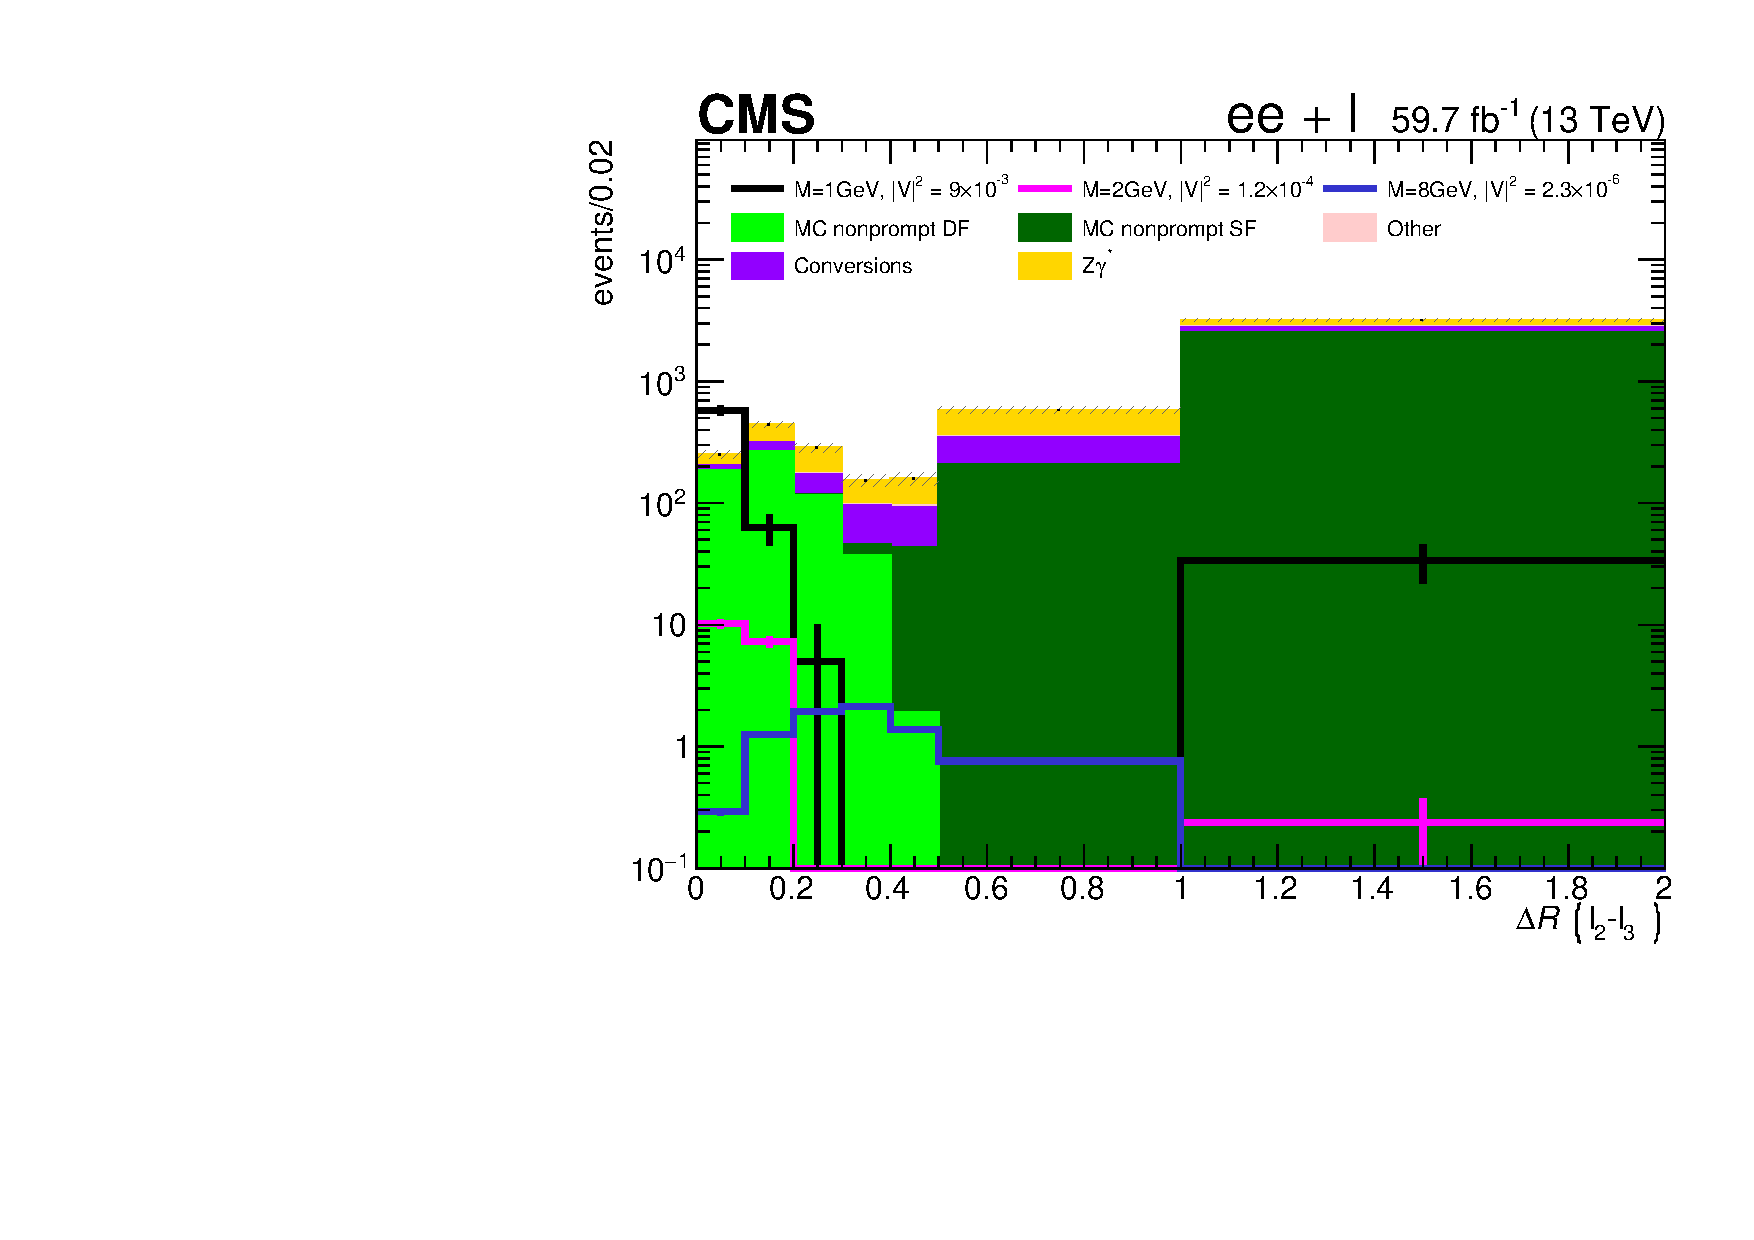
\includegraphics[width=.28\textwidth]{Figures/c6/selection/18/e_DeltaR_l2_l3__0.pdf}
  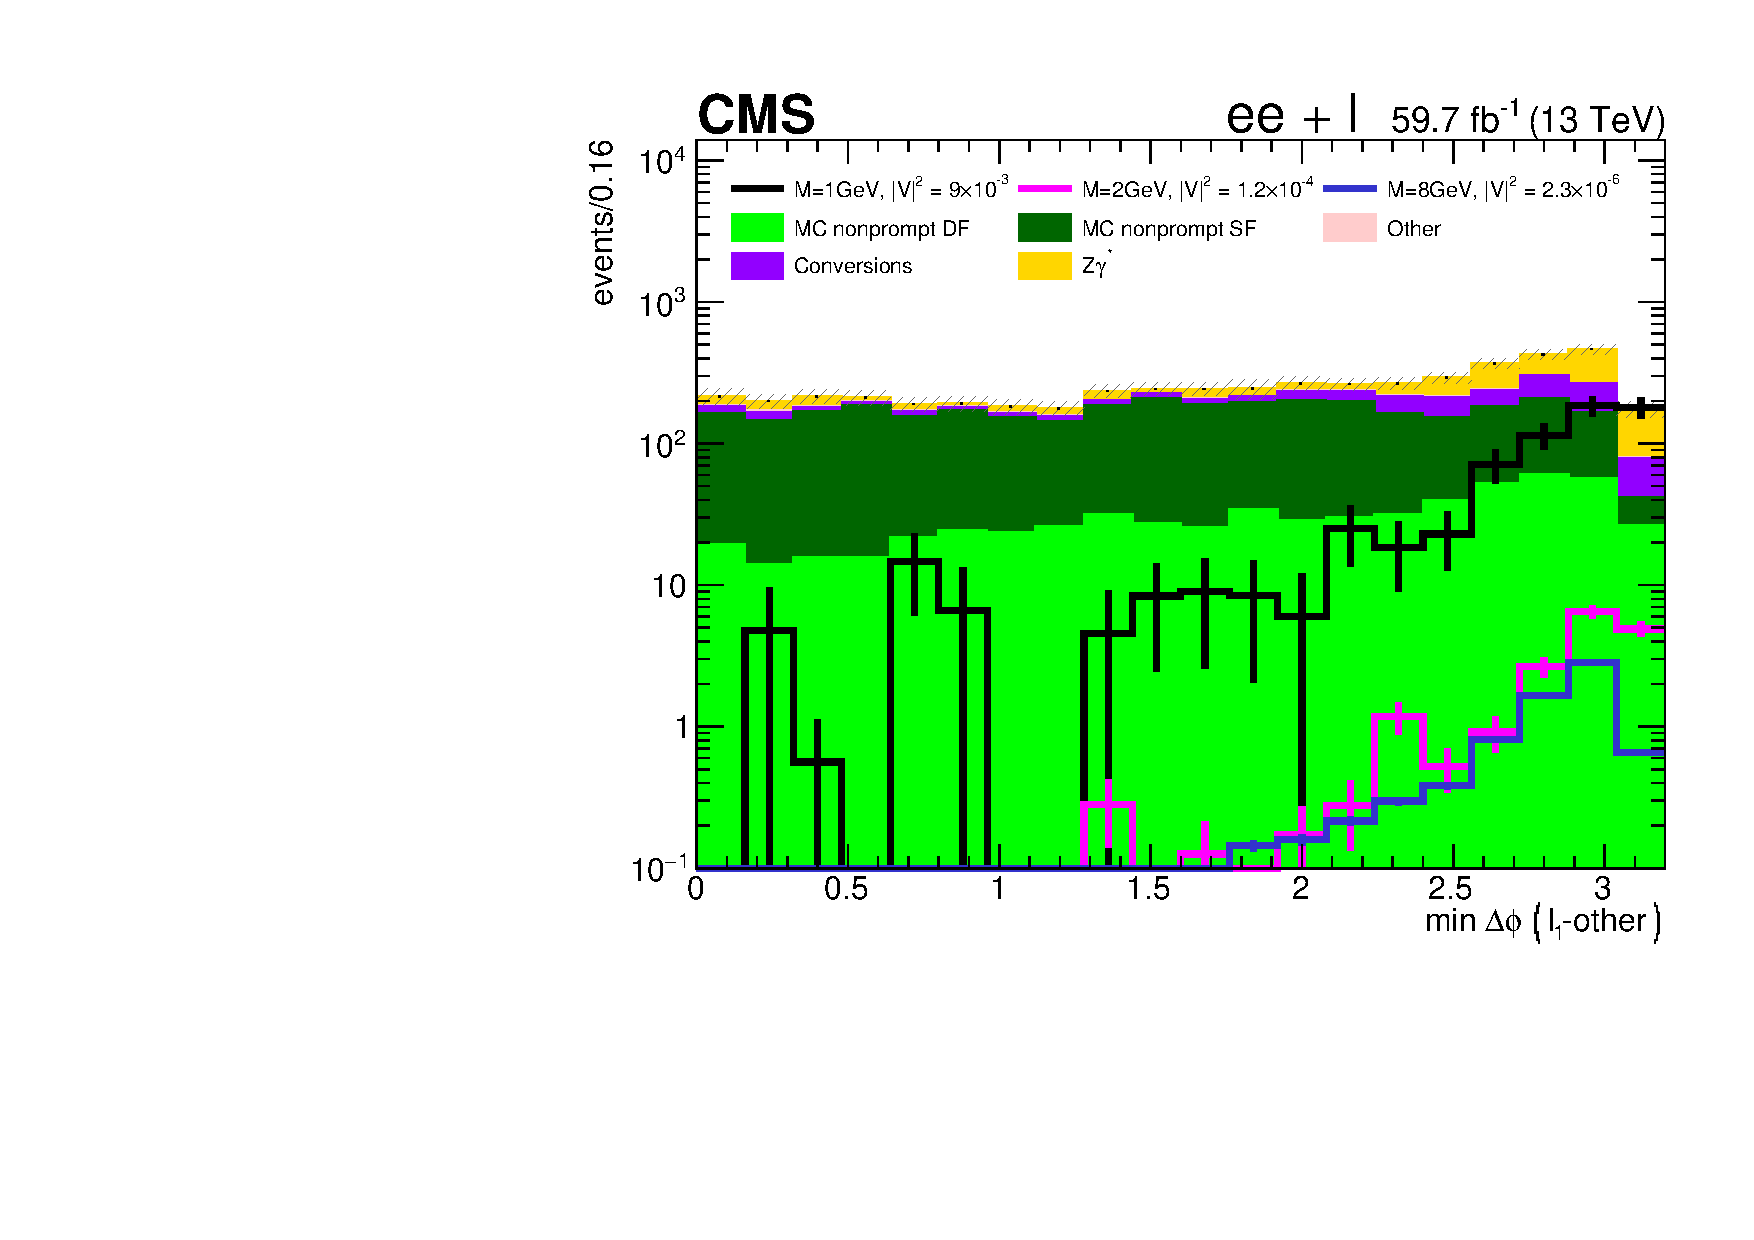
\includegraphics[width=.28\textwidth]{Figures/c6/selection/18/e_minDeltaphil1_other__0.pdf}
  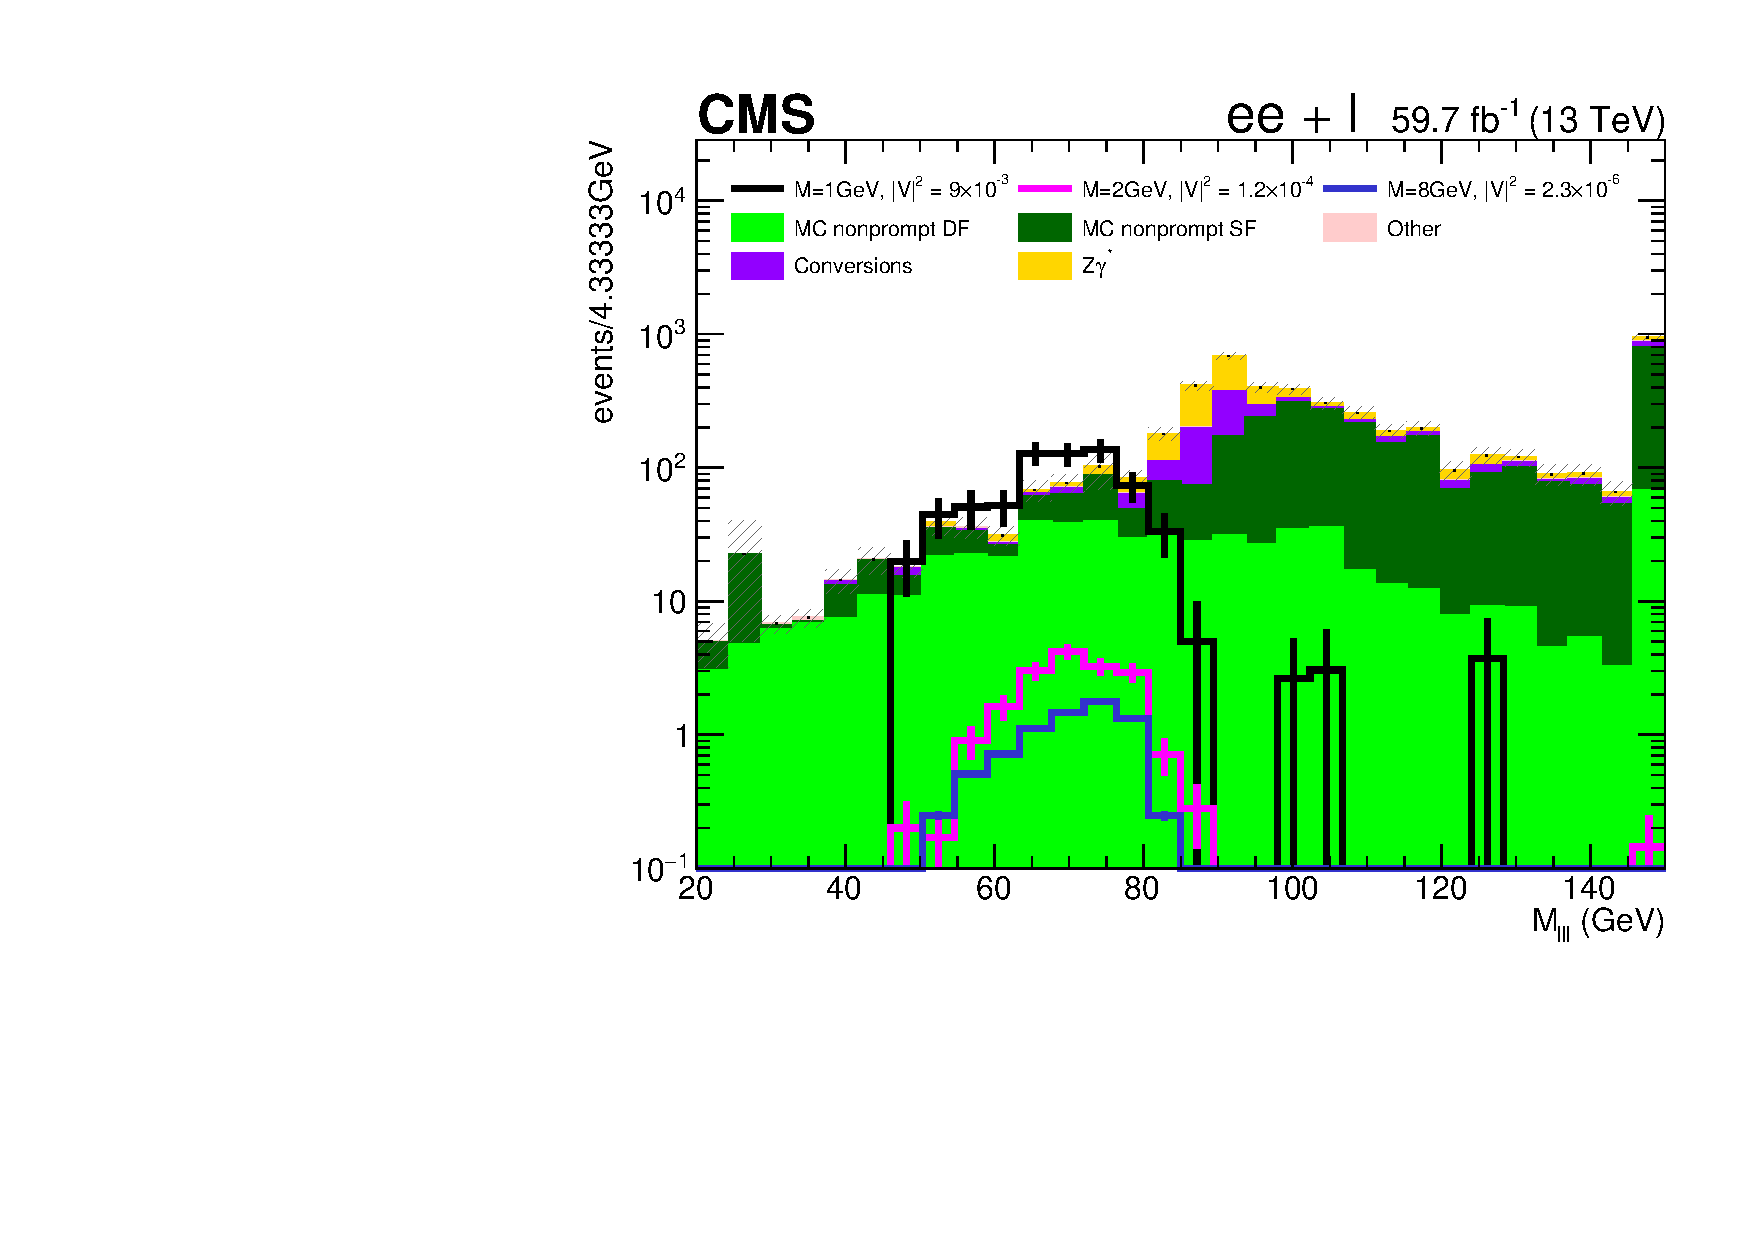
\includegraphics[width=.28\textwidth]{Figures/c6/selection/18/e_M_lll__0.pdf}
  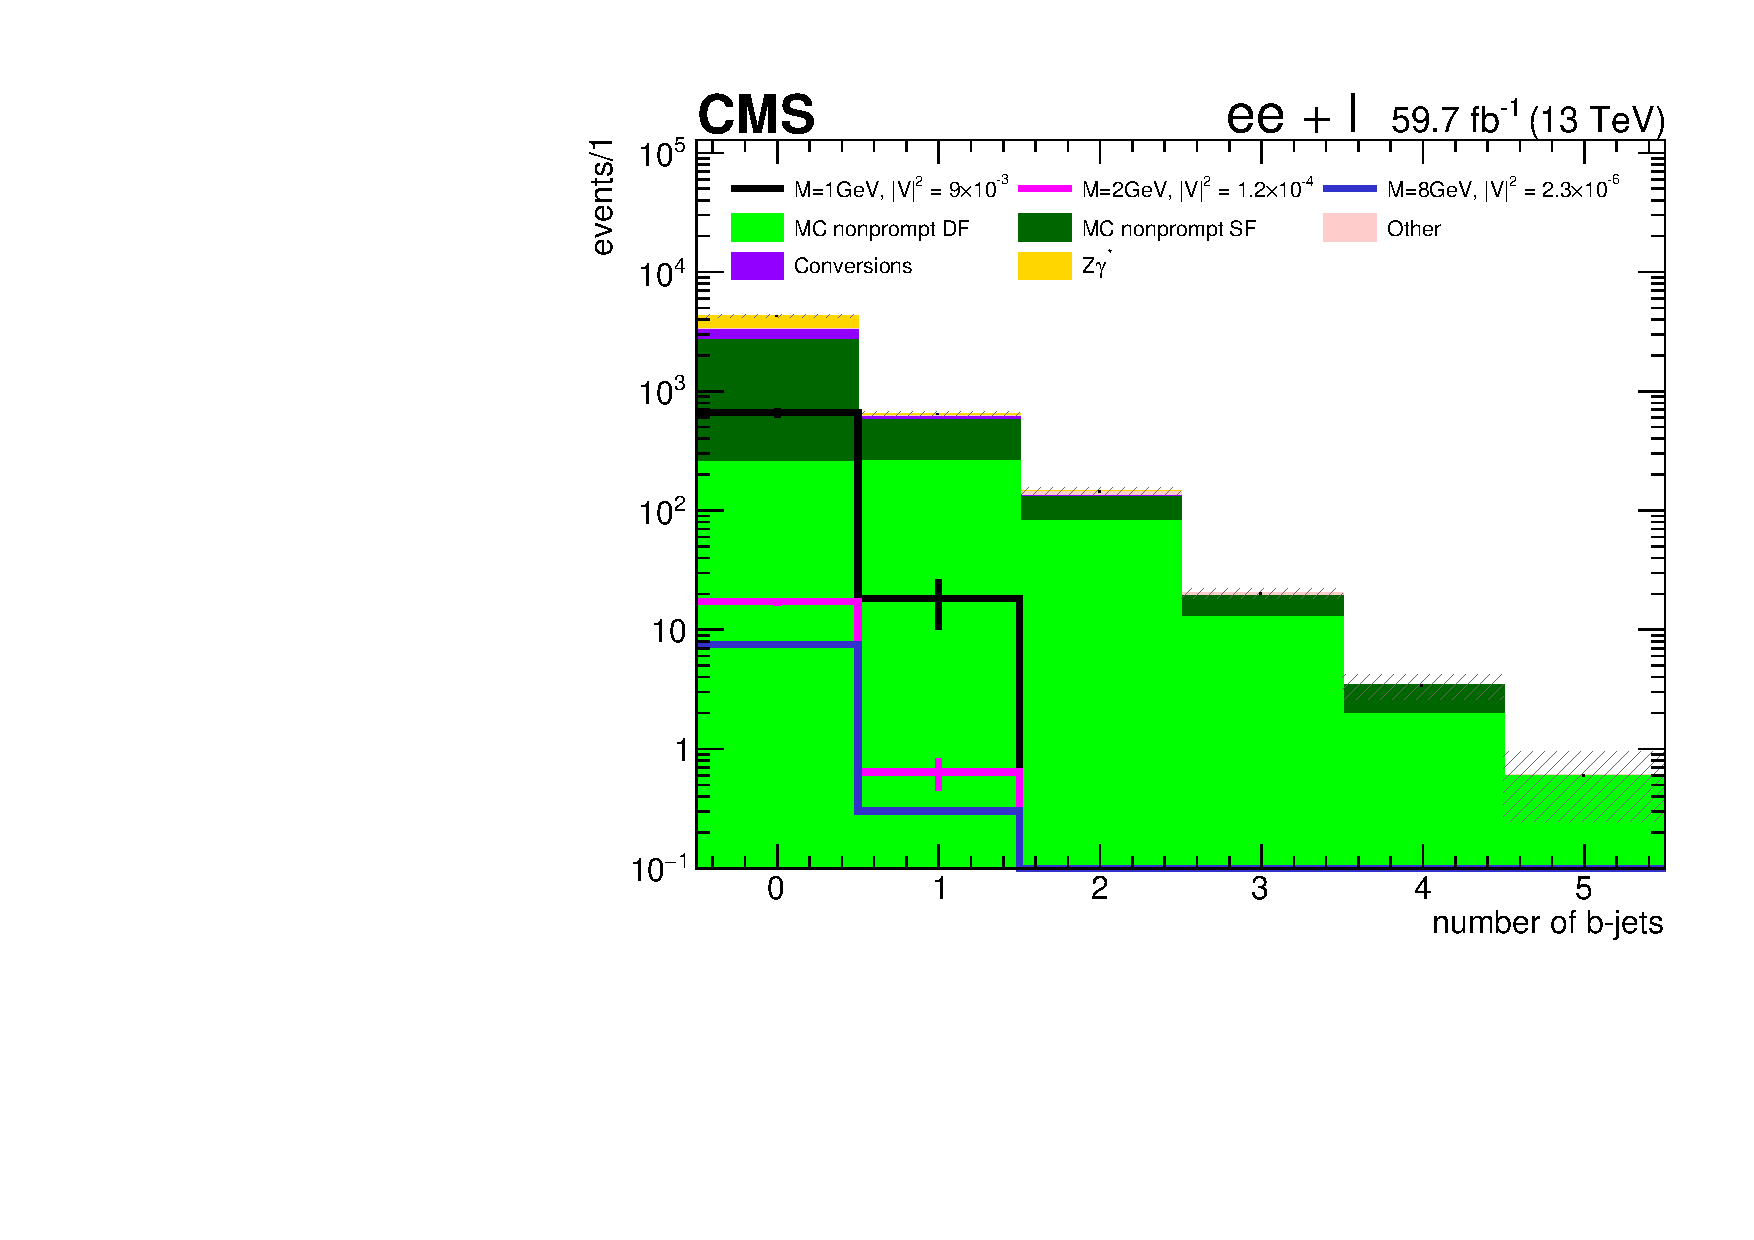
\includegraphics[width=.28\textwidth]{Figures/c6/selection/18/e_numberofb_jets__0.pdf}}\\
\makebox[\textwidth]{
  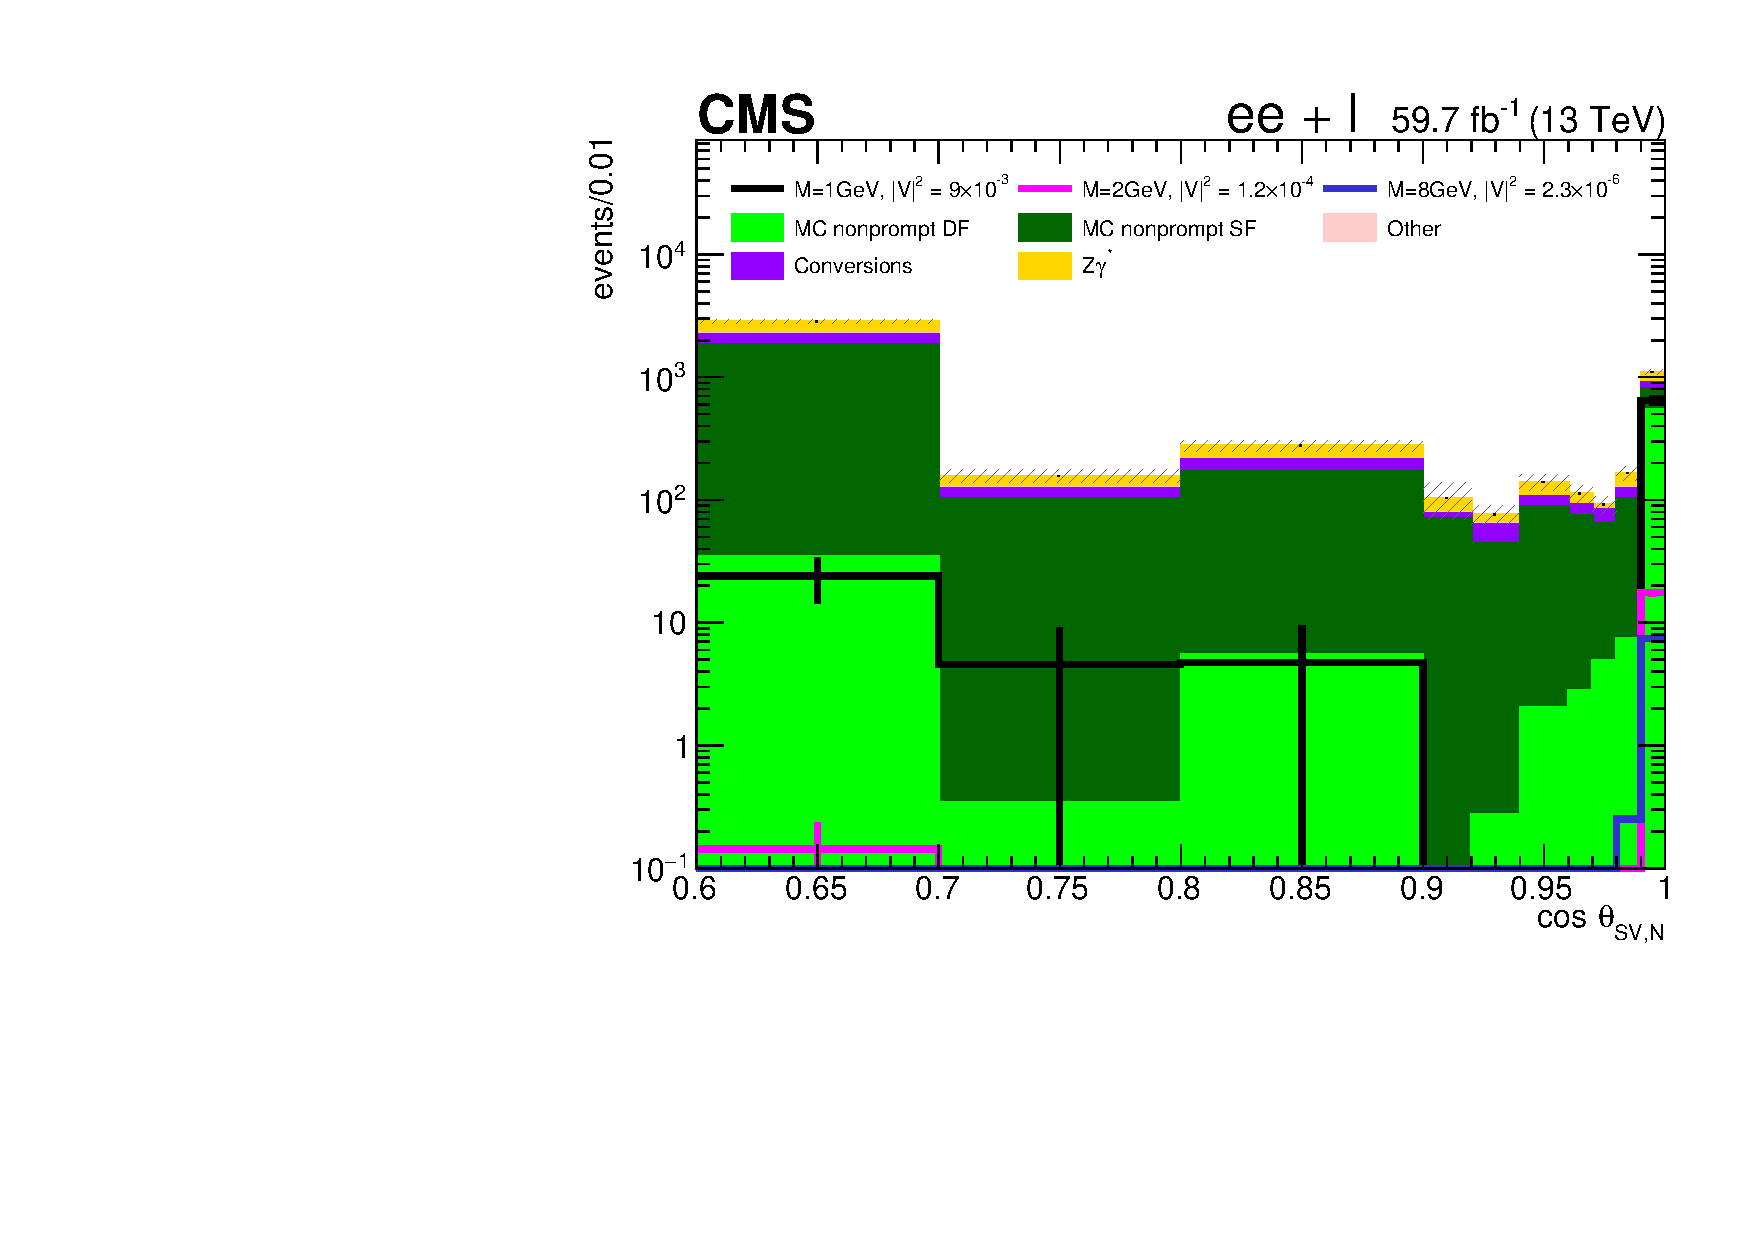
\includegraphics[width=.28\textwidth]{Figures/c6/selection/18/e_cosSVposl2_l3dir__0.pdf}
  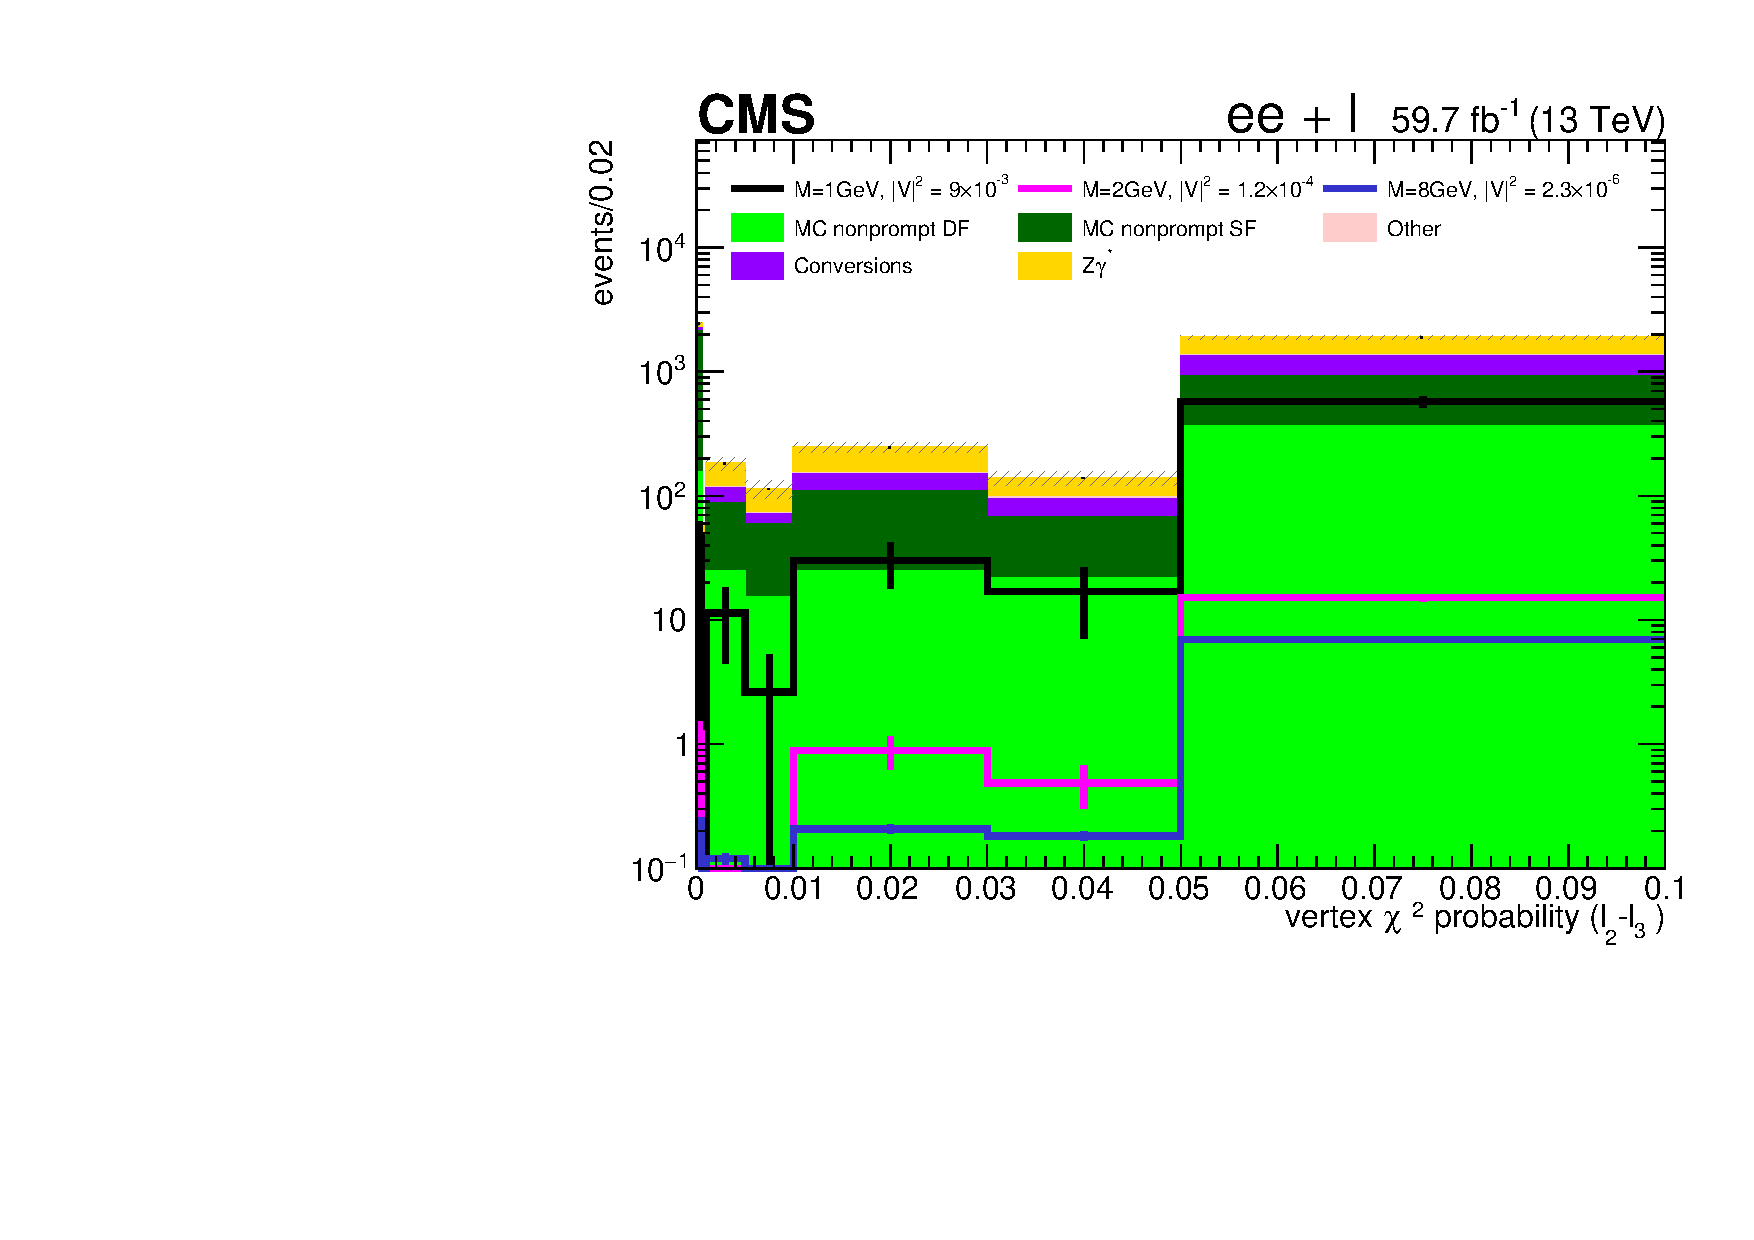
\includegraphics[width=.28\textwidth]{Figures/c6/selection/18/e_vertexchi2_probabilityl2_l3__0.pdf}
  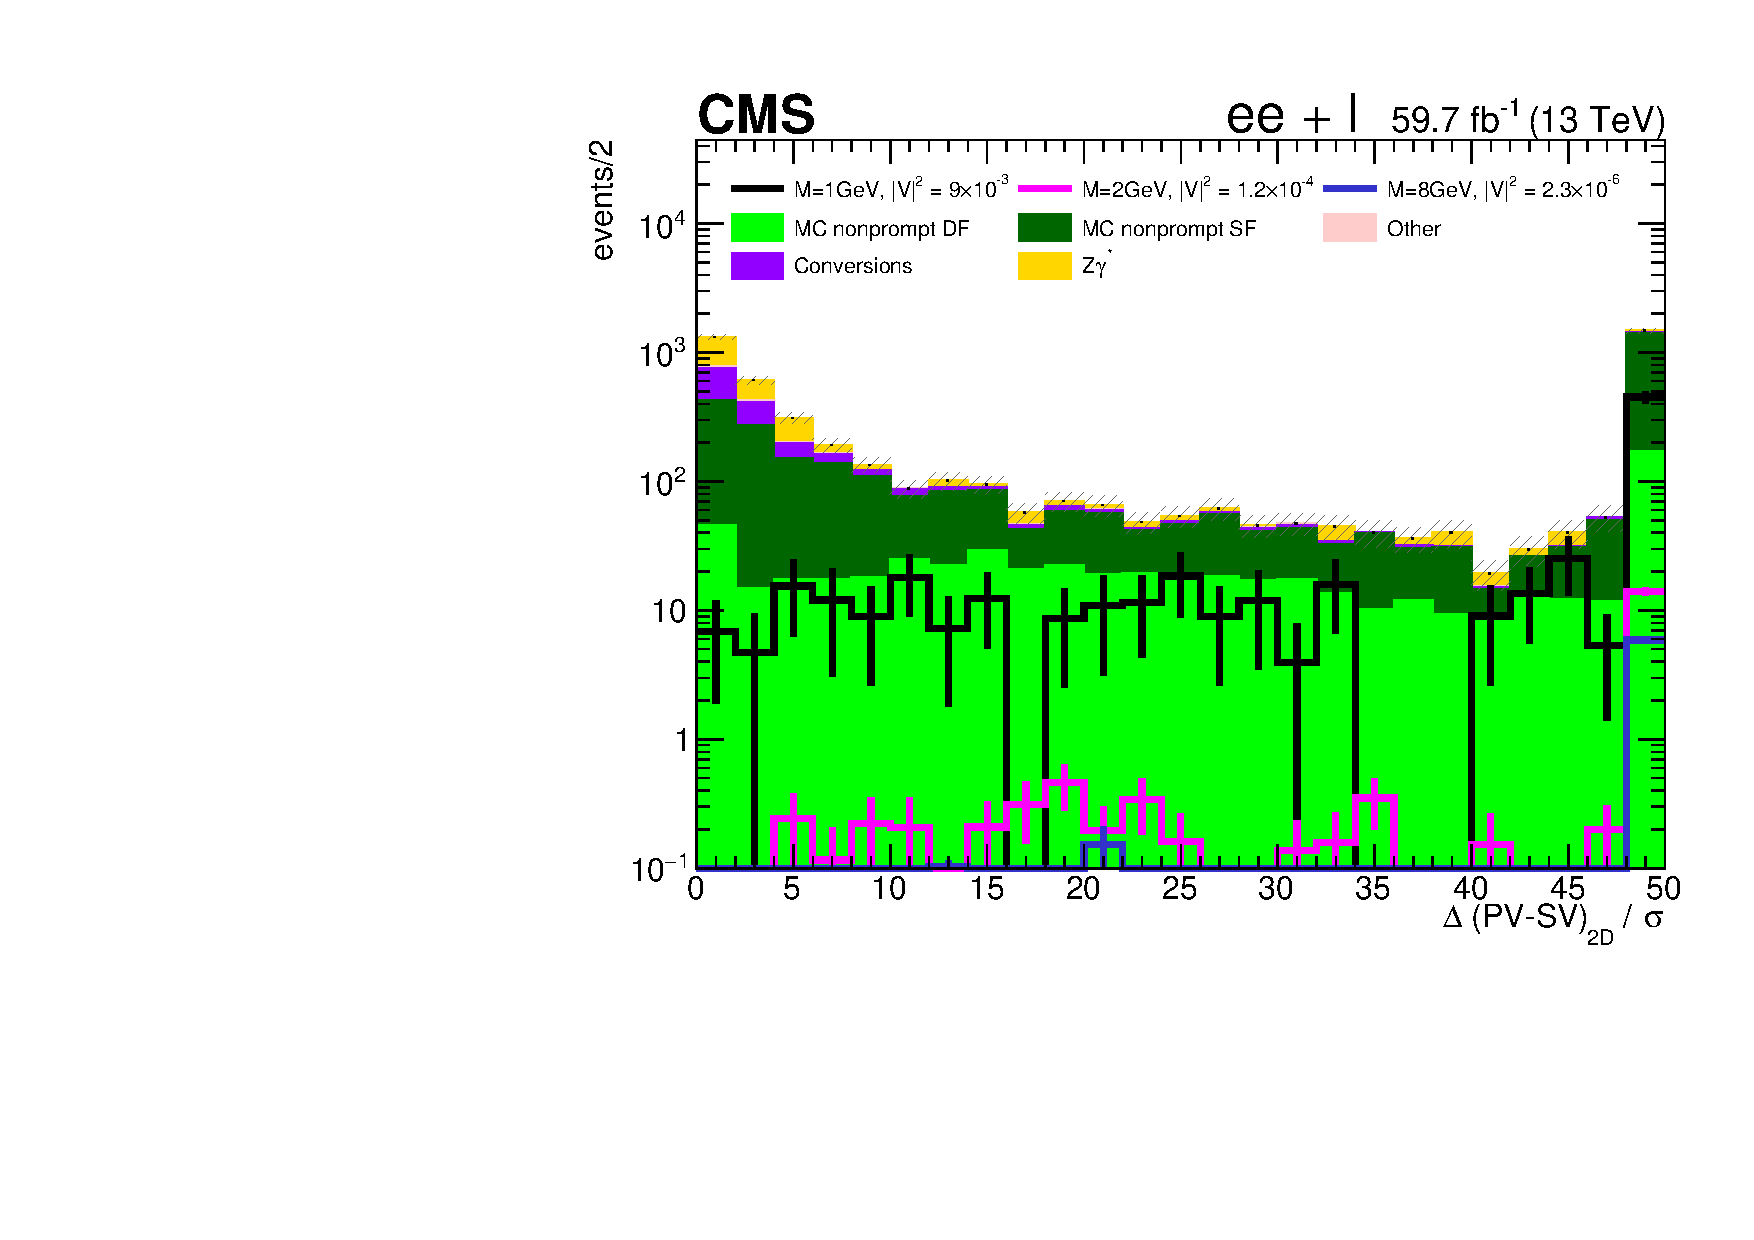
\includegraphics[width=.28\textwidth]{Figures/c6/selection/18/e_sigmaDeltaPV_SV_2D__0.pdf}
  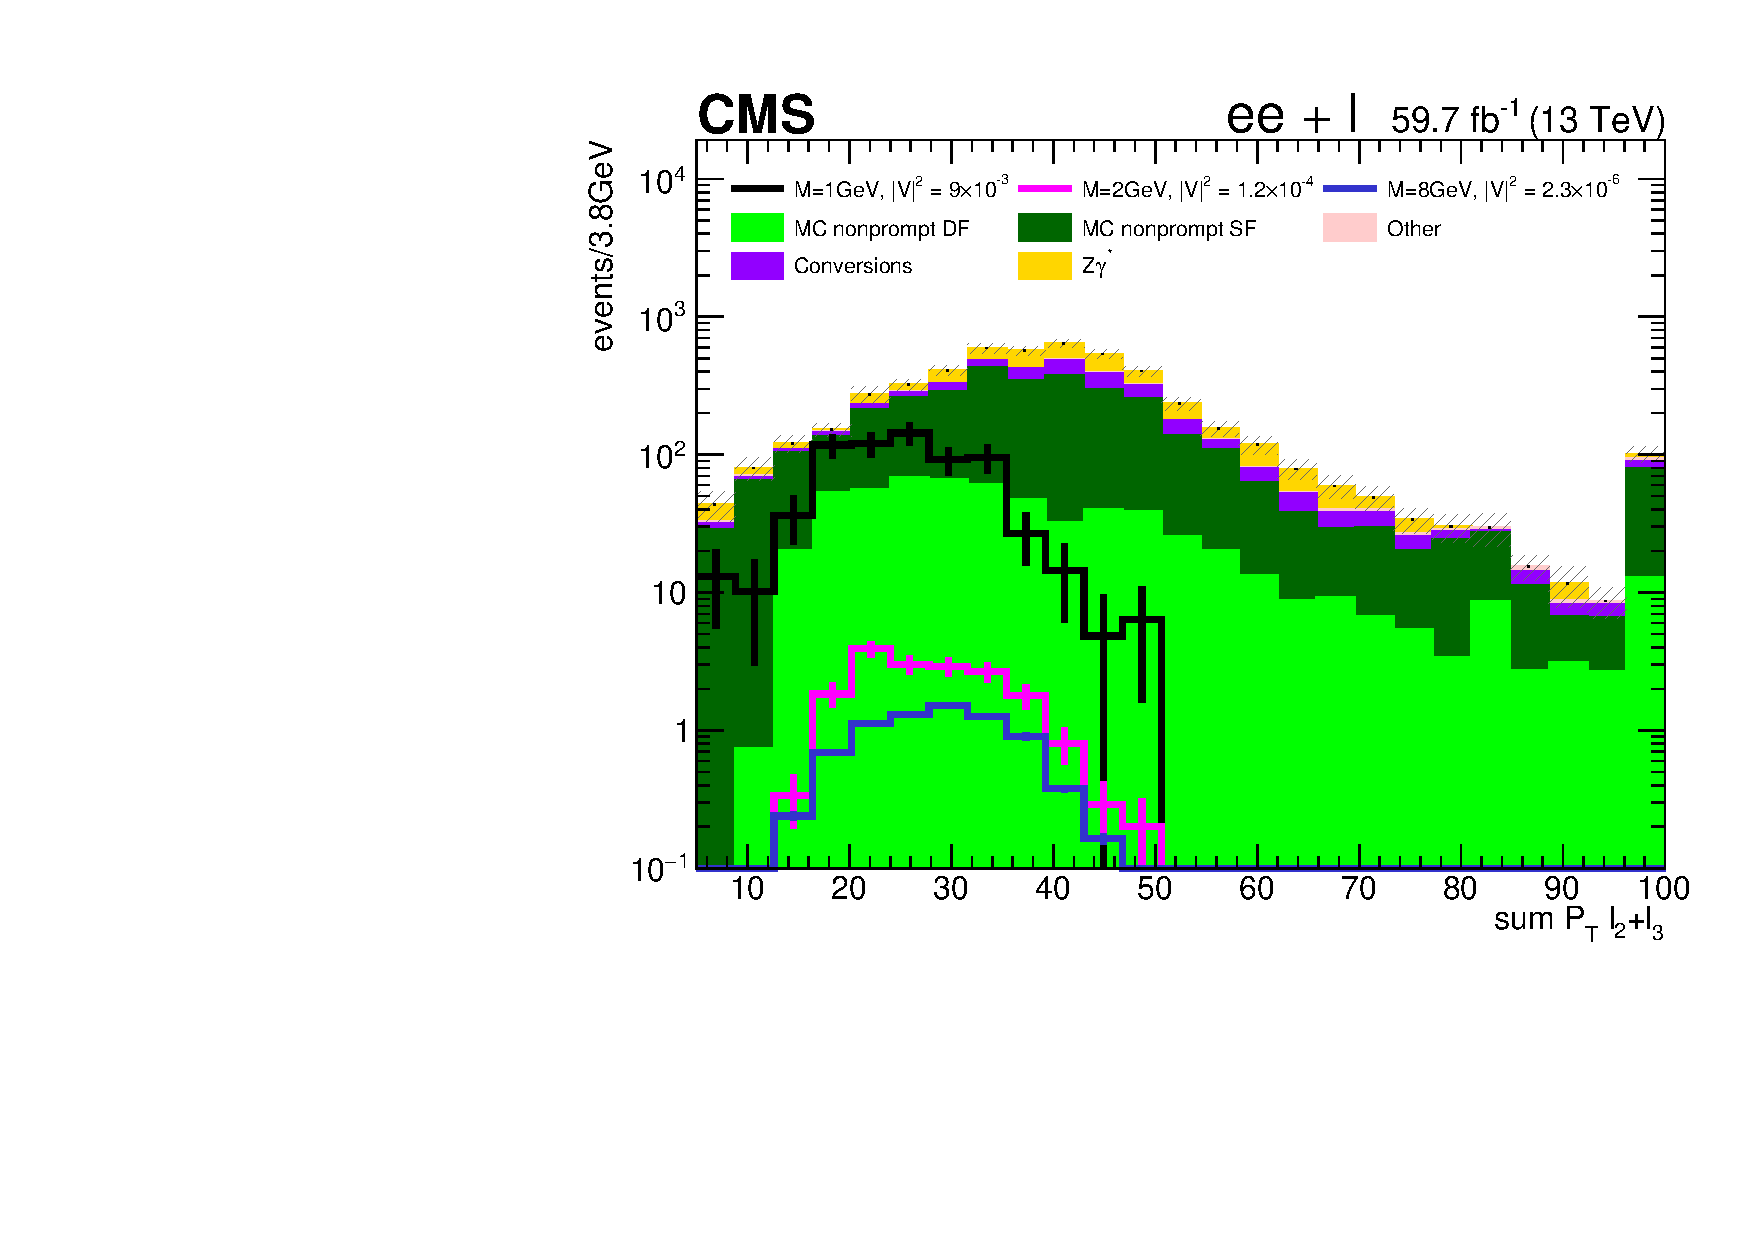
\includegraphics[width=.28\textwidth]{Figures/c6/selection/18/e_sum_Pt_L2L3__0.pdf}}\\
  \caption{Distributions of the event selection's variables listed in
    Table~\ref{tab:baselinesel}. Simulated backgrounds (shaded histograms, stacked),
    using the 2018 MC samples, 
    after the selection of the three leptons \lone, \ltwo, and \lthree,
    in \eex final states.
    Signal models for different values of \mhnl and \mixpar are shown
    as empty histograms.}
  \label{fig:selection_electrons}
\end{figure}

\begin{figure}[h]
\noindent
\makebox[\textwidth]{
  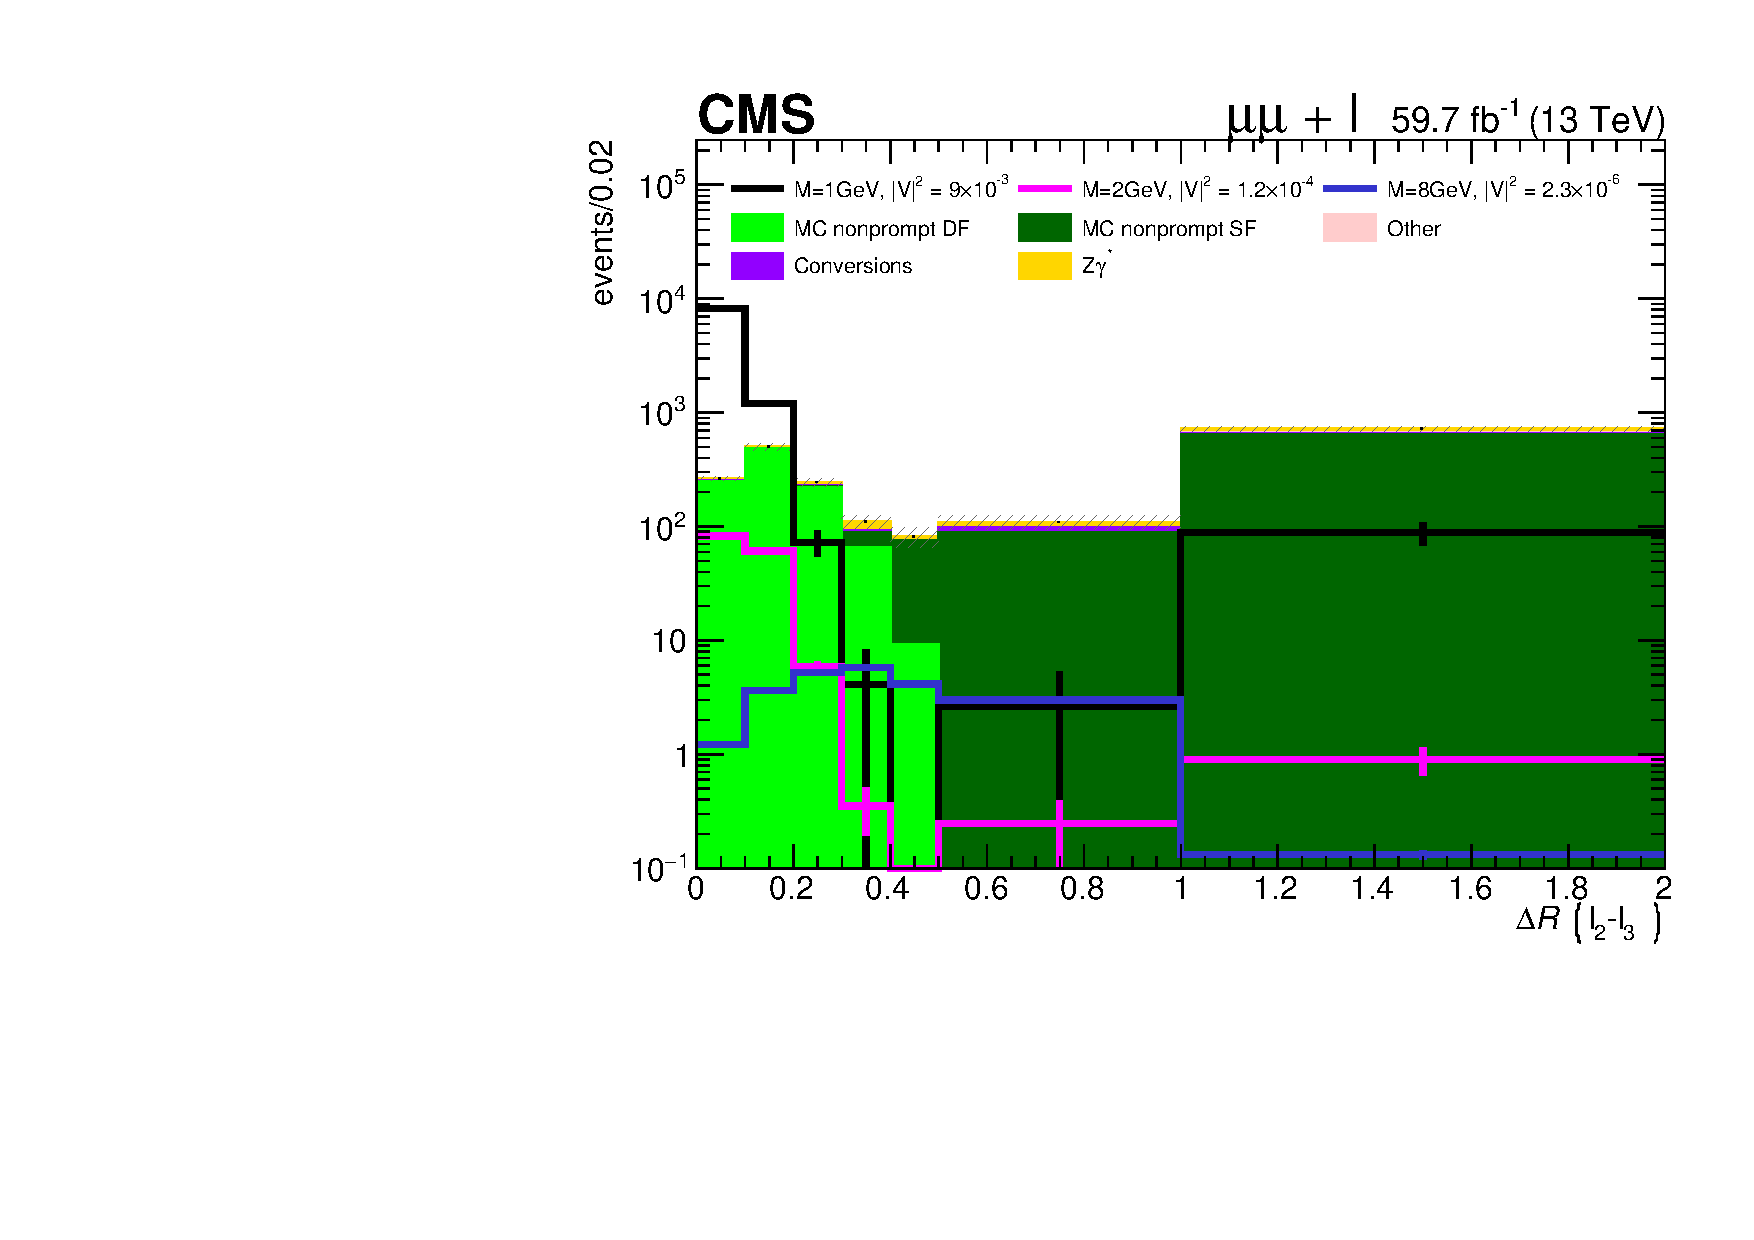
\includegraphics[width=.28\textwidth]{Figures/c6/selection/18/mu_DeltaR_l2_l3__0.pdf}
  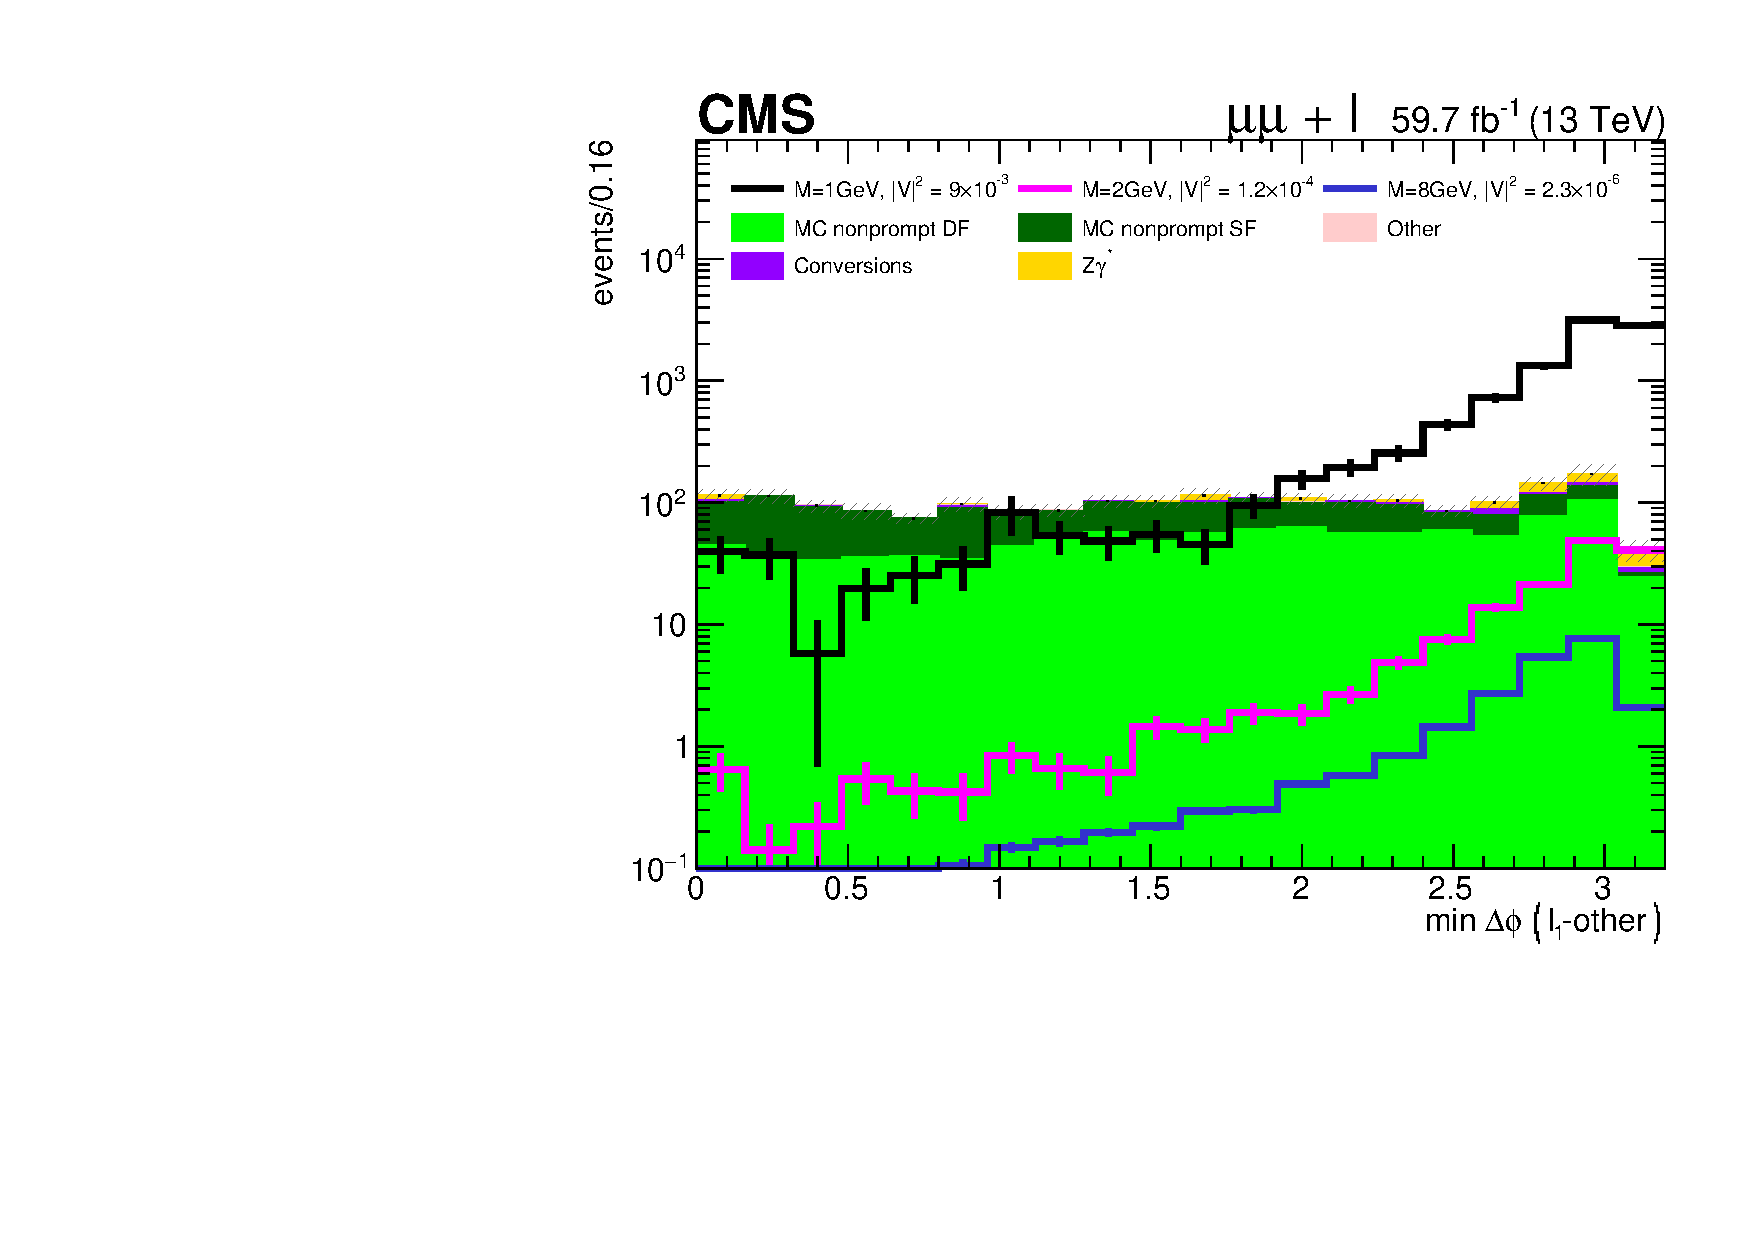
\includegraphics[width=.28\textwidth]{Figures/c6/selection/18/mu_minDeltaphil1_other__0.pdf}
  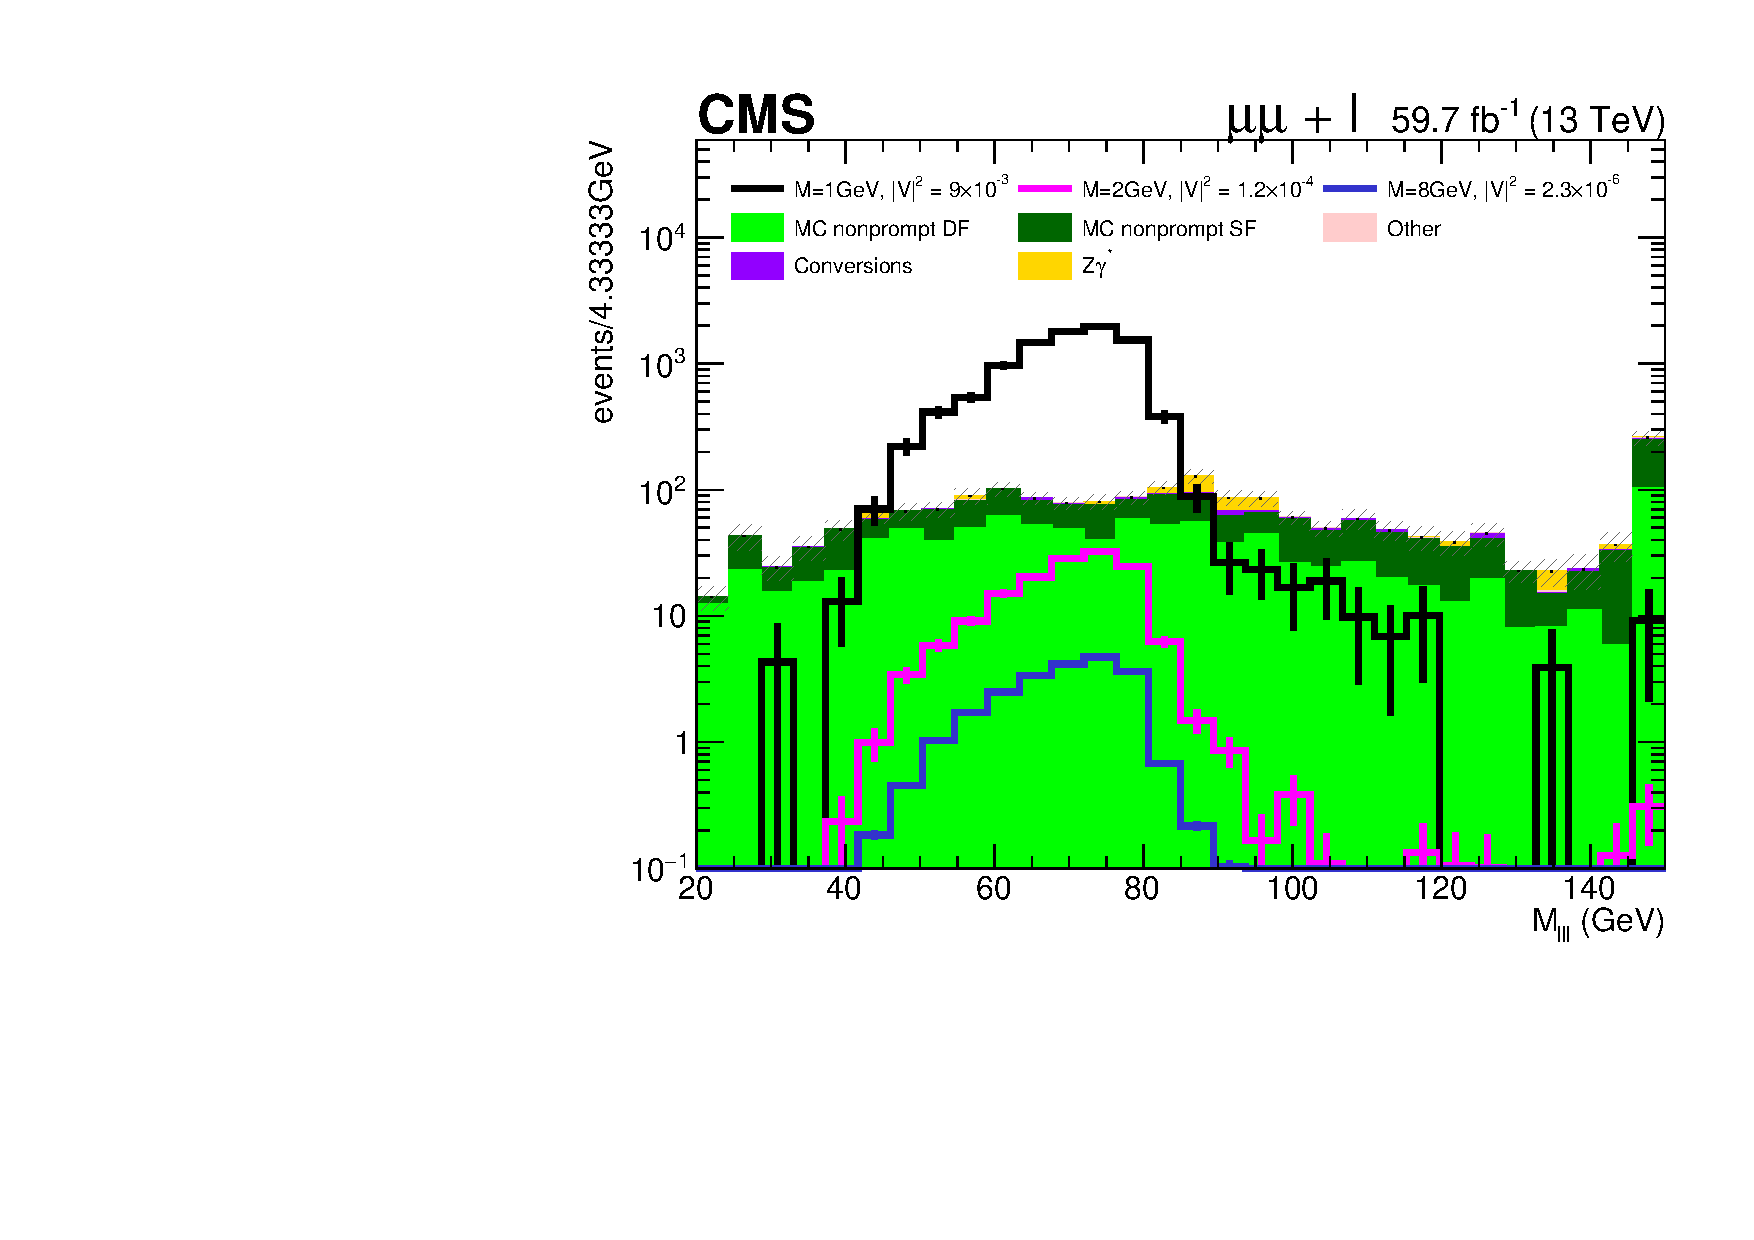
\includegraphics[width=.28\textwidth]{Figures/c6/selection/18/mu_M_lll__0.pdf}
  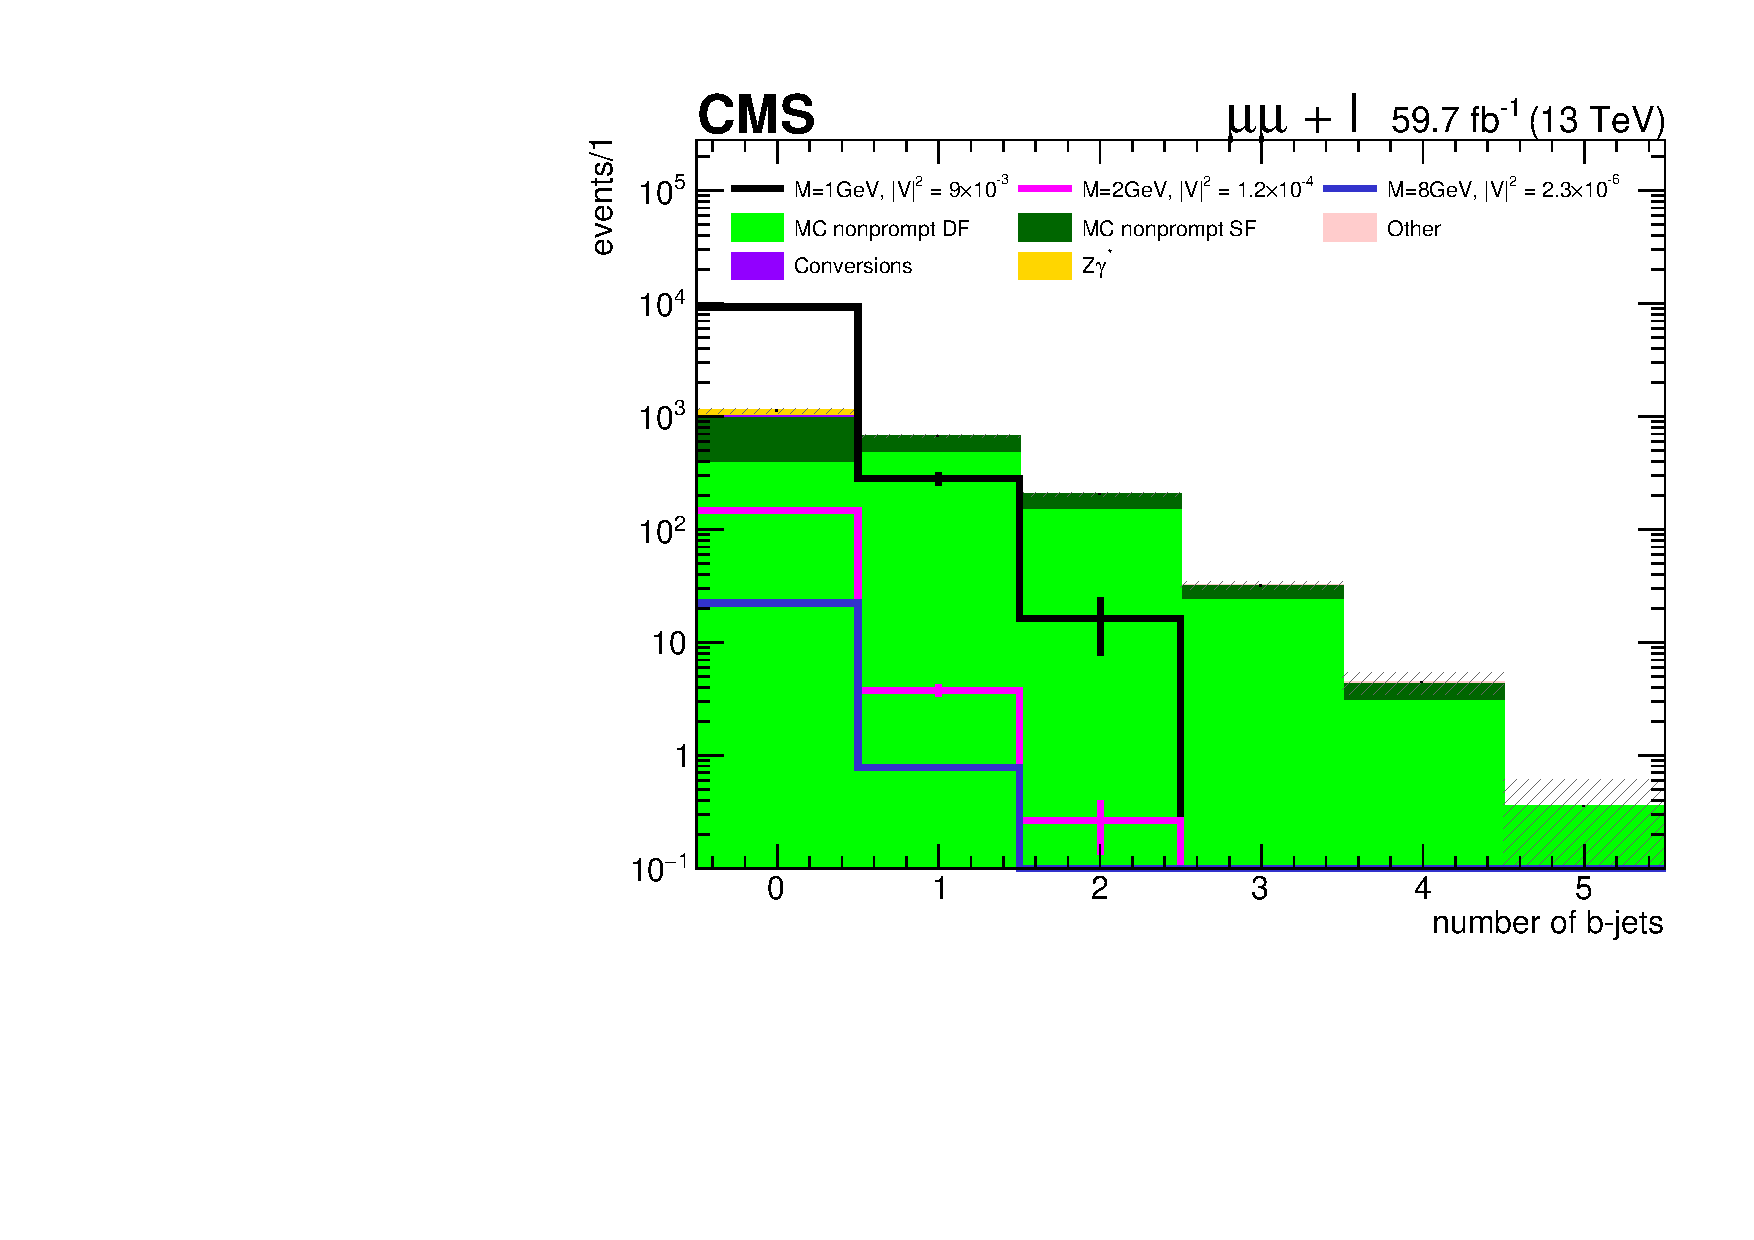
\includegraphics[width=.28\textwidth]{Figures/c6/selection/18/mu_numberofb_jets__0.pdf}}\\
\makebox[\textwidth]{
  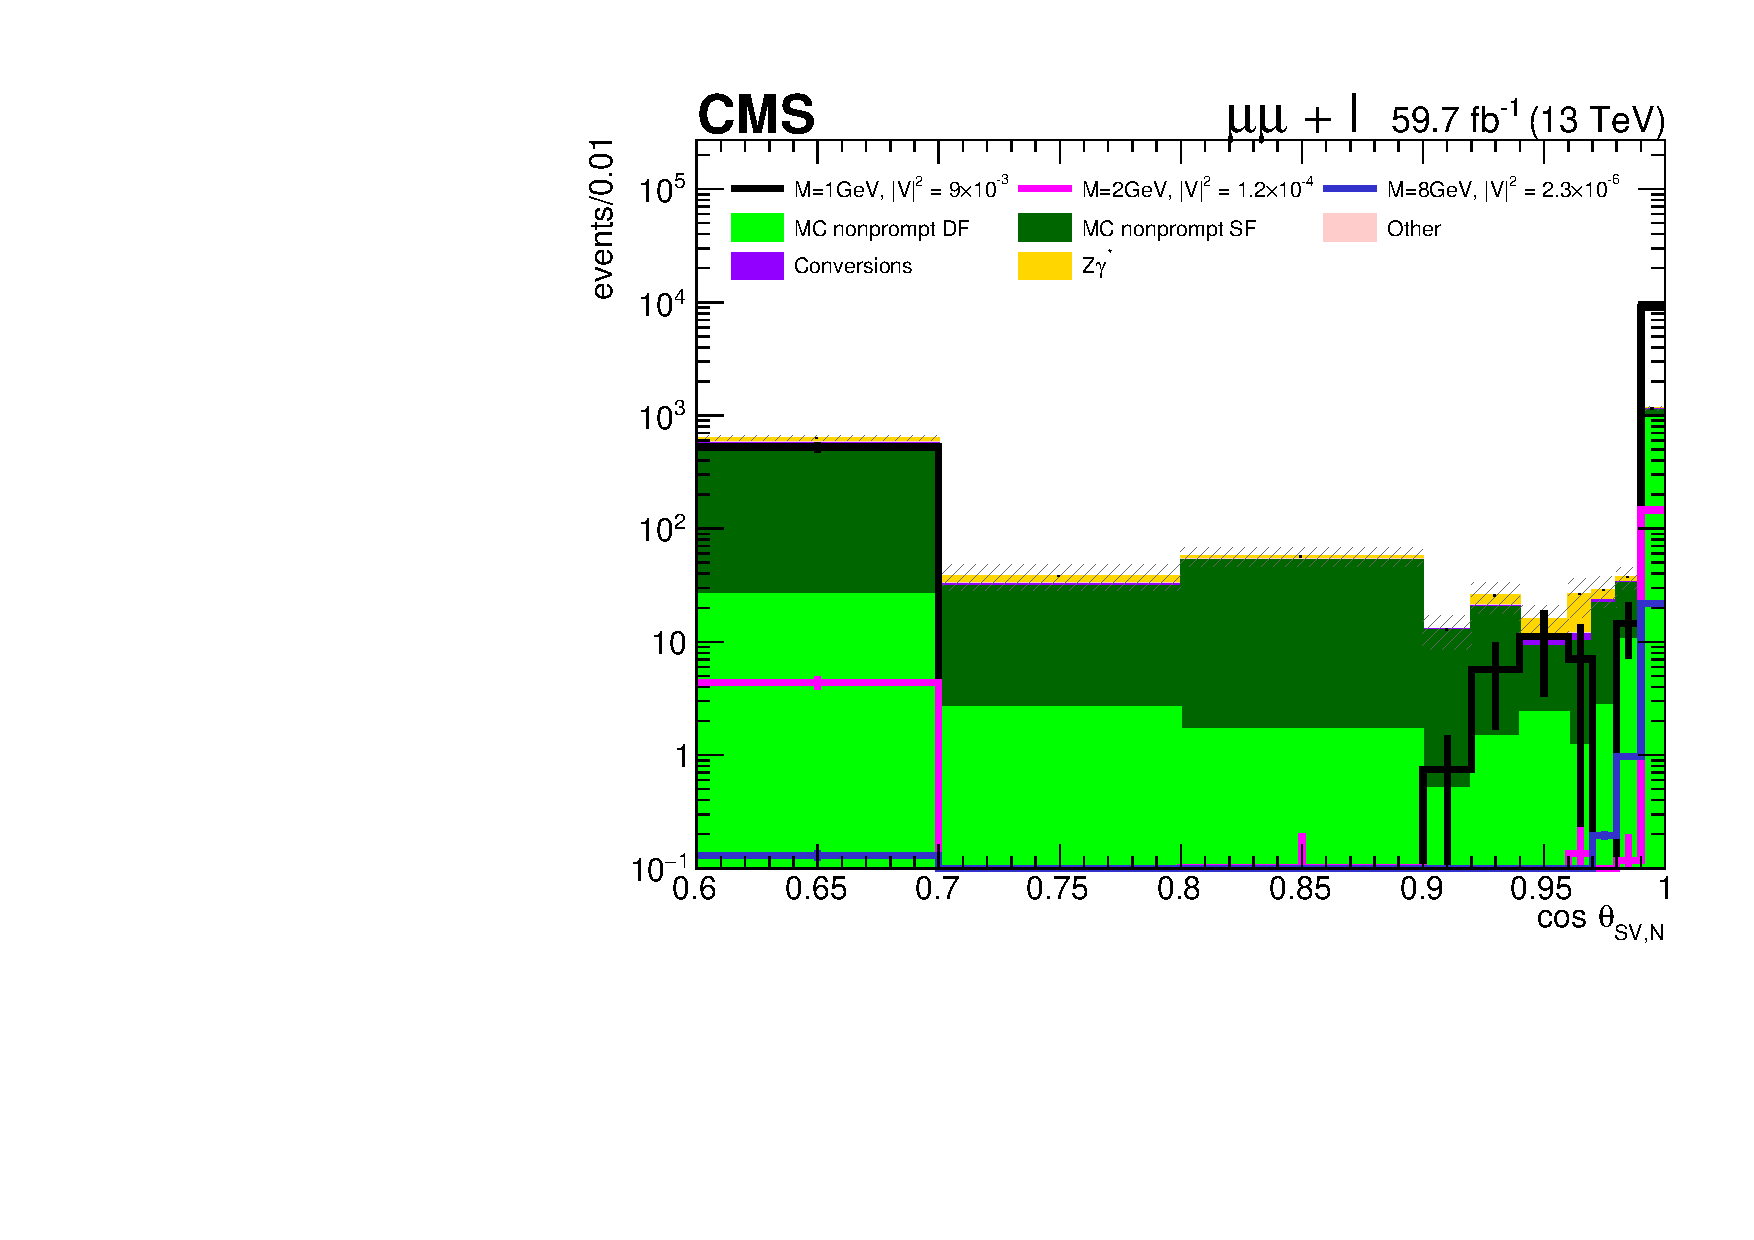
\includegraphics[width=.28\textwidth]{Figures/c6/selection/18/mu_cosSVposl2_l3dir__0.pdf}
  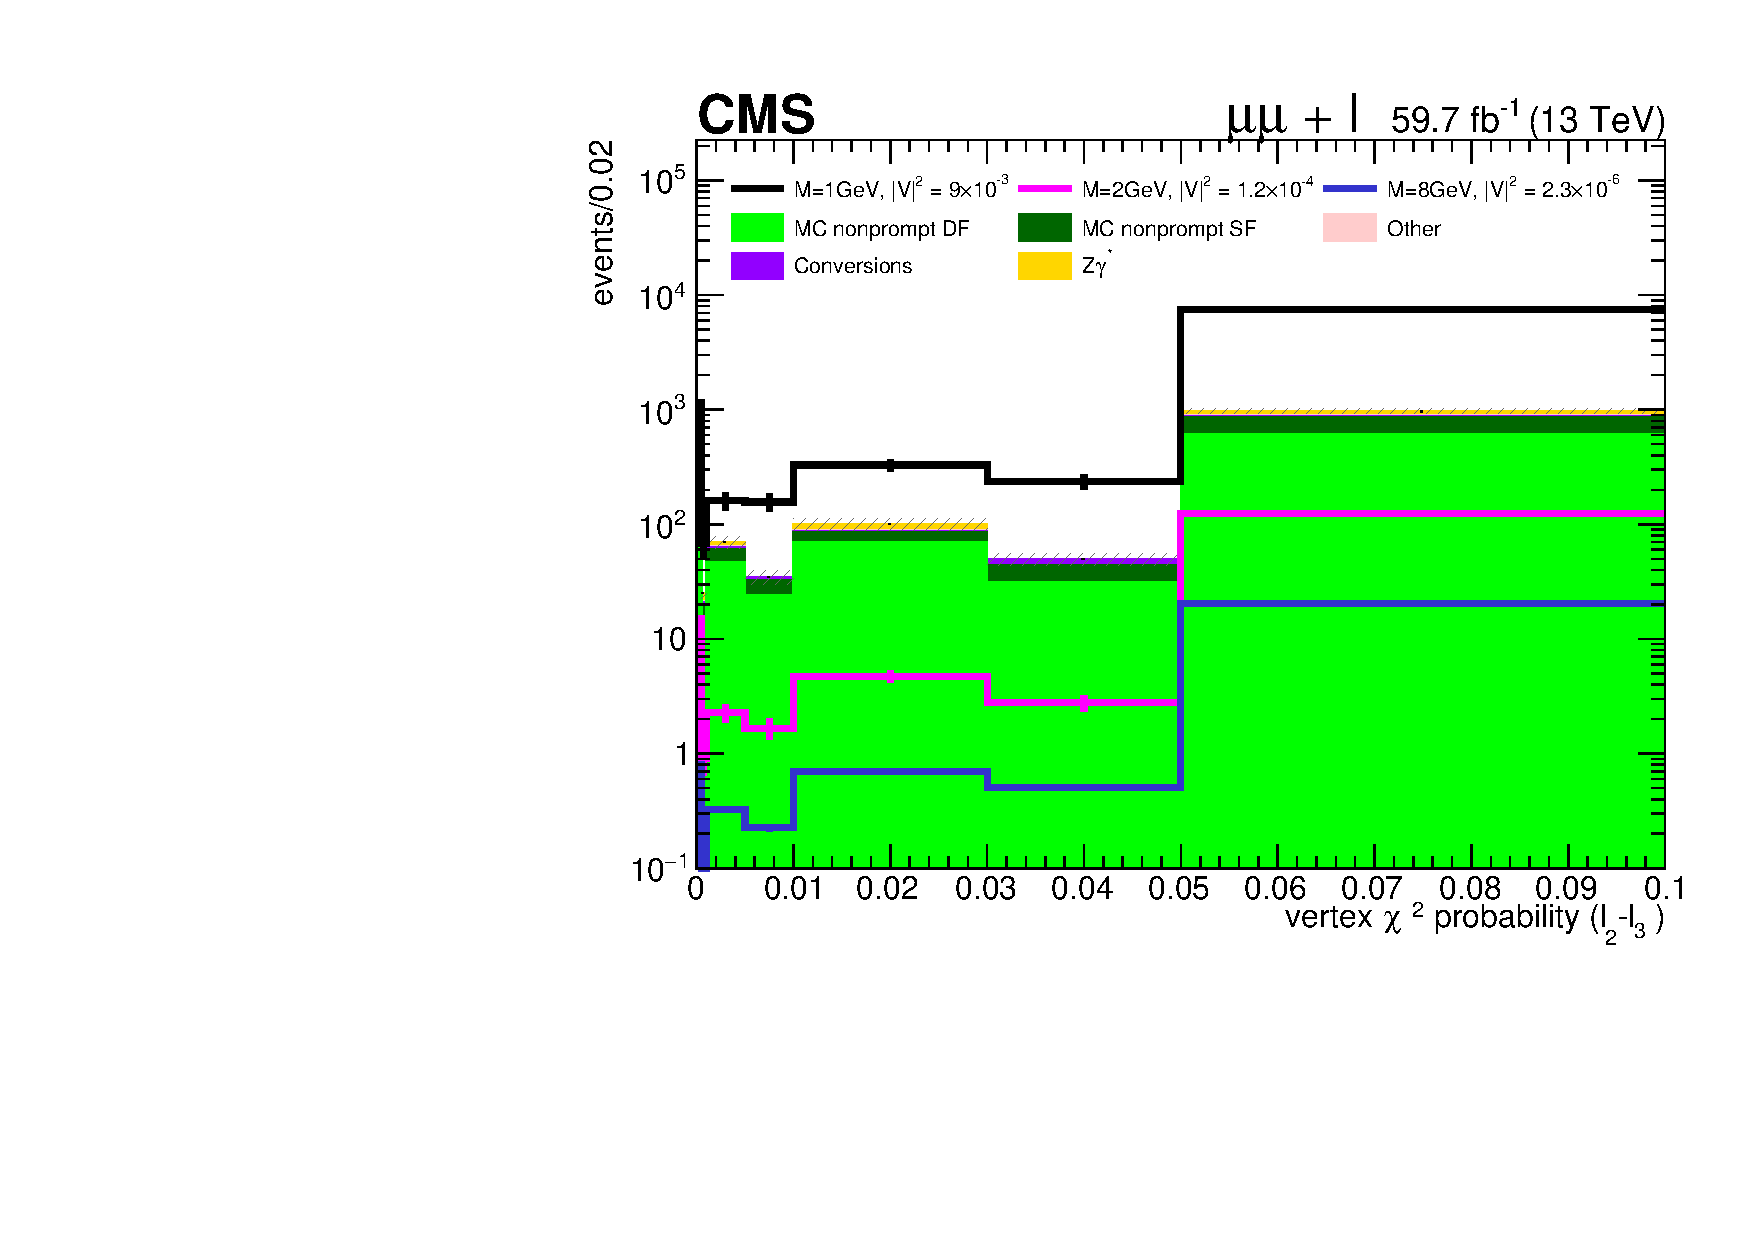
\includegraphics[width=.28\textwidth]{Figures/c6/selection/18/mu_vertexchi2_probabilityl2_l3__0.pdf}
  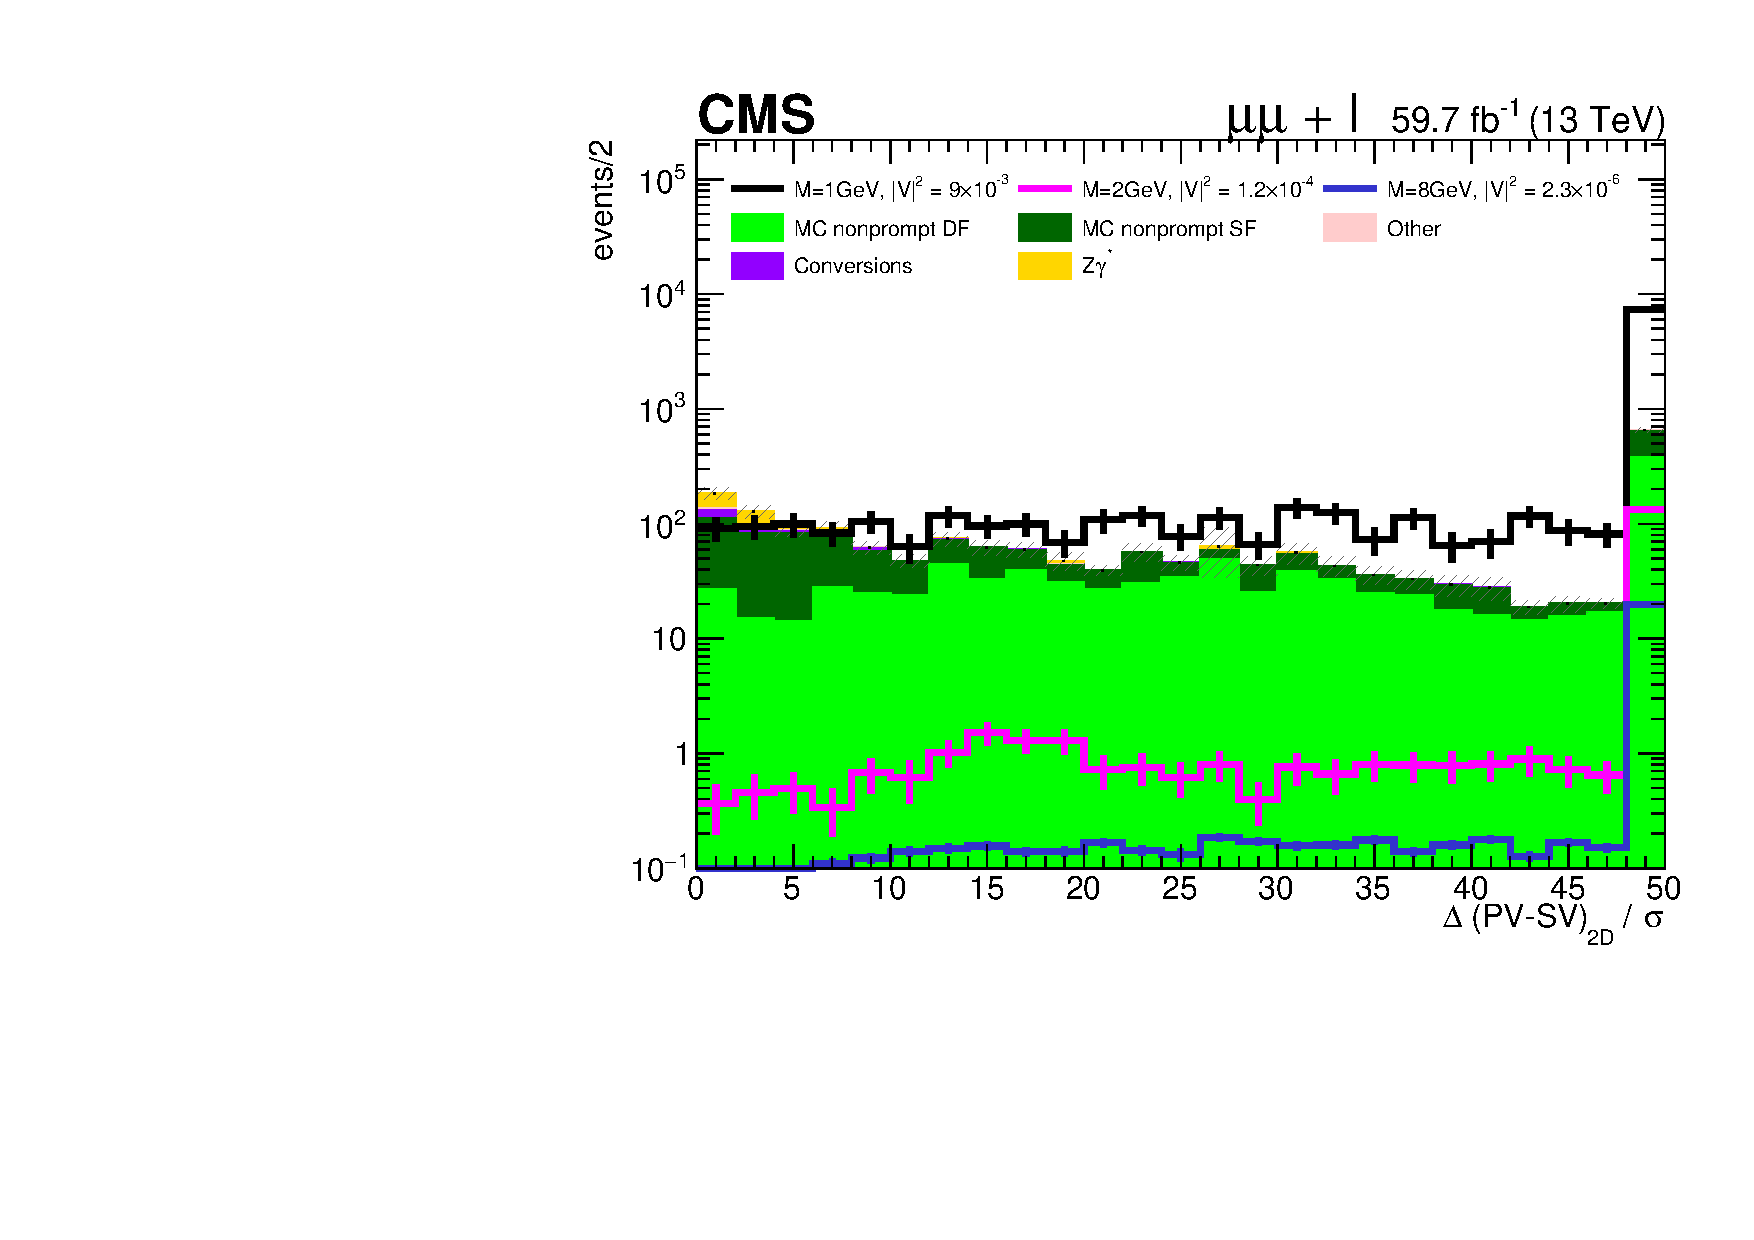
\includegraphics[width=.28\textwidth]{Figures/c6/selection/18/mu_sigmaDeltaPV_SV_2D__0.pdf}
  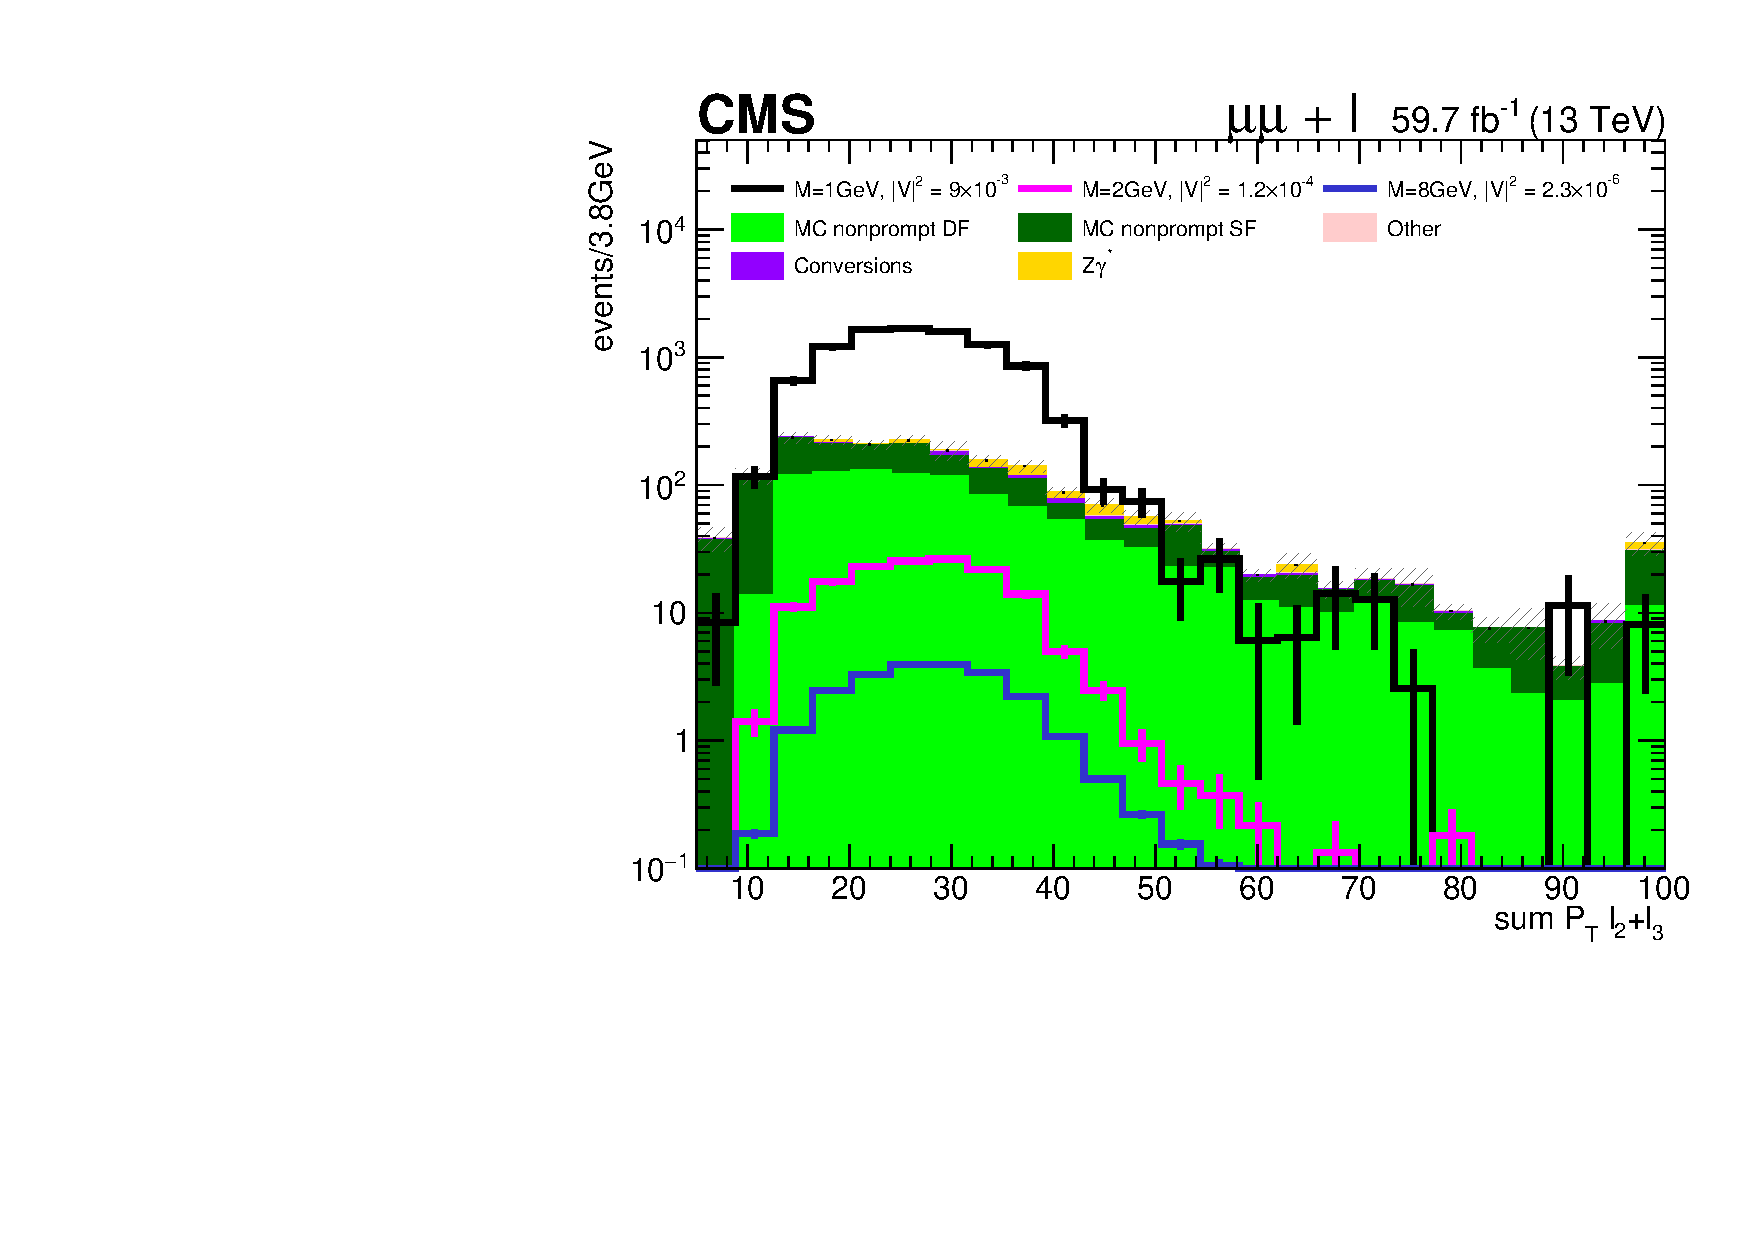
\includegraphics[width=.28\textwidth]{Figures/c6/selection/18/mu_sum_Pt_L2L3__0.pdf}}\\
  \caption{Distributions of the event selection's variables listed in
    Table~\ref{tab:baselinesel}. Simulated backgrounds (shaded histograms, stacked),
    using the 2018 MC samples, 
    after the selection of the three leptons \lone, \ltwo, and \lthree,
    in \mmx final states.
    Signal models for different values of \mhnl and \mixpar are shown
    as empty histograms.}
  \label{fig:selection_muons}
\end{figure}

The following plots are a summary view of the entire selection
(~\ref{tab:baselinesel}) showing two different kind of "cutflows". The
first set, fig~\ref{fig:cutflow1}, is the classic cutflow where each
bin displays the number of left events after each cut and it goes in a
"cascade" way (one after the other). The second one,
fig~\ref{fig:cutflow2}, is a $N-1$ plot where each bin has the number
of events when that particular cut is not applied; in this way it is
possible to appreciate which is the real impact of each cut no matter
its position in the even selection list. 

As it is seen in Fig.~\ref{fig:cutflow1}, the most effective background rejection is achieved with the \mthreel selection. It is in particular effective in \eex final states as it rejects DY events where at least one electron comes from conversion. In such events \mthreel populates the region of $M_{\PZ}$ which remains outside the [40-80]\GeV signal region.

\begin{figure}[h]
  \noindent
  \makebox[\textwidth]{
  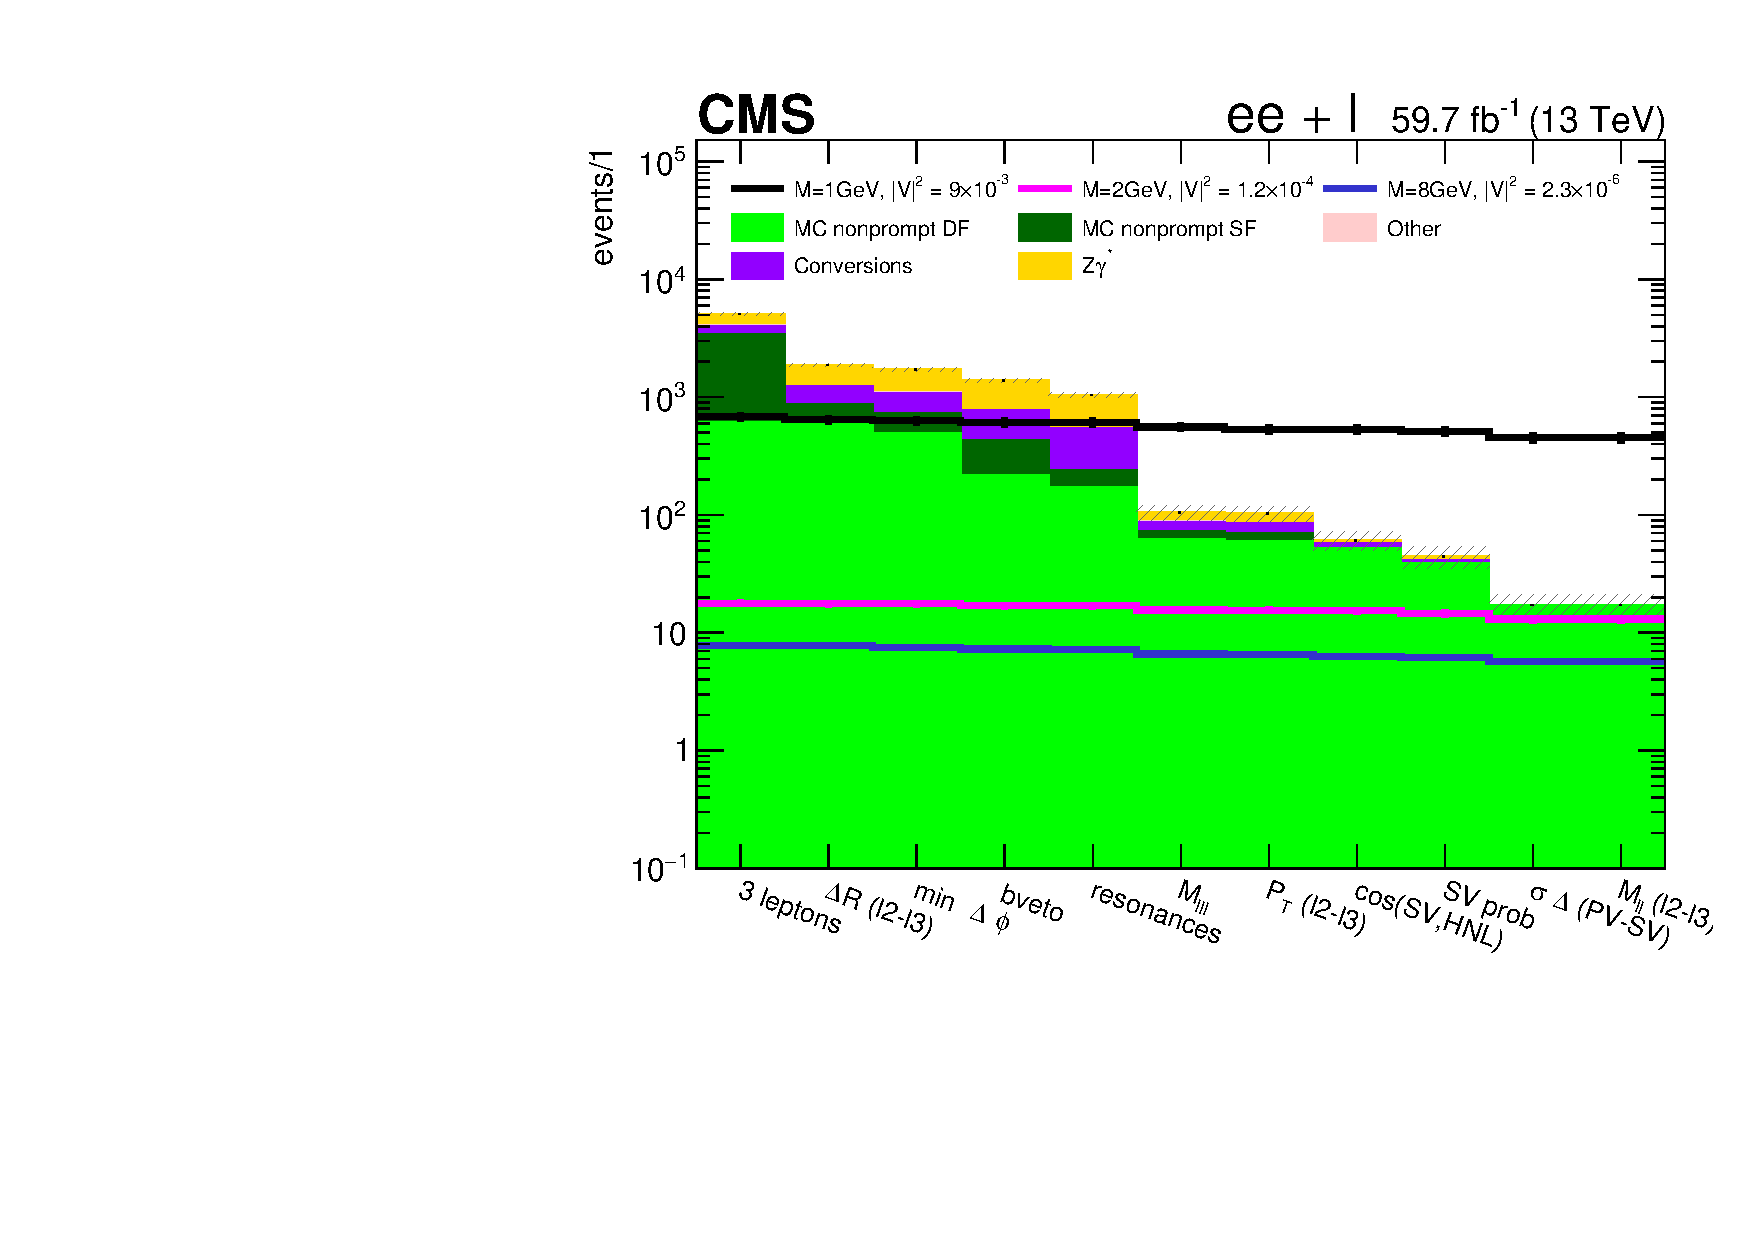
\includegraphics[width=.34\textwidth]{Figures/c6/selection/18/e_cutflow__0.pdf}
  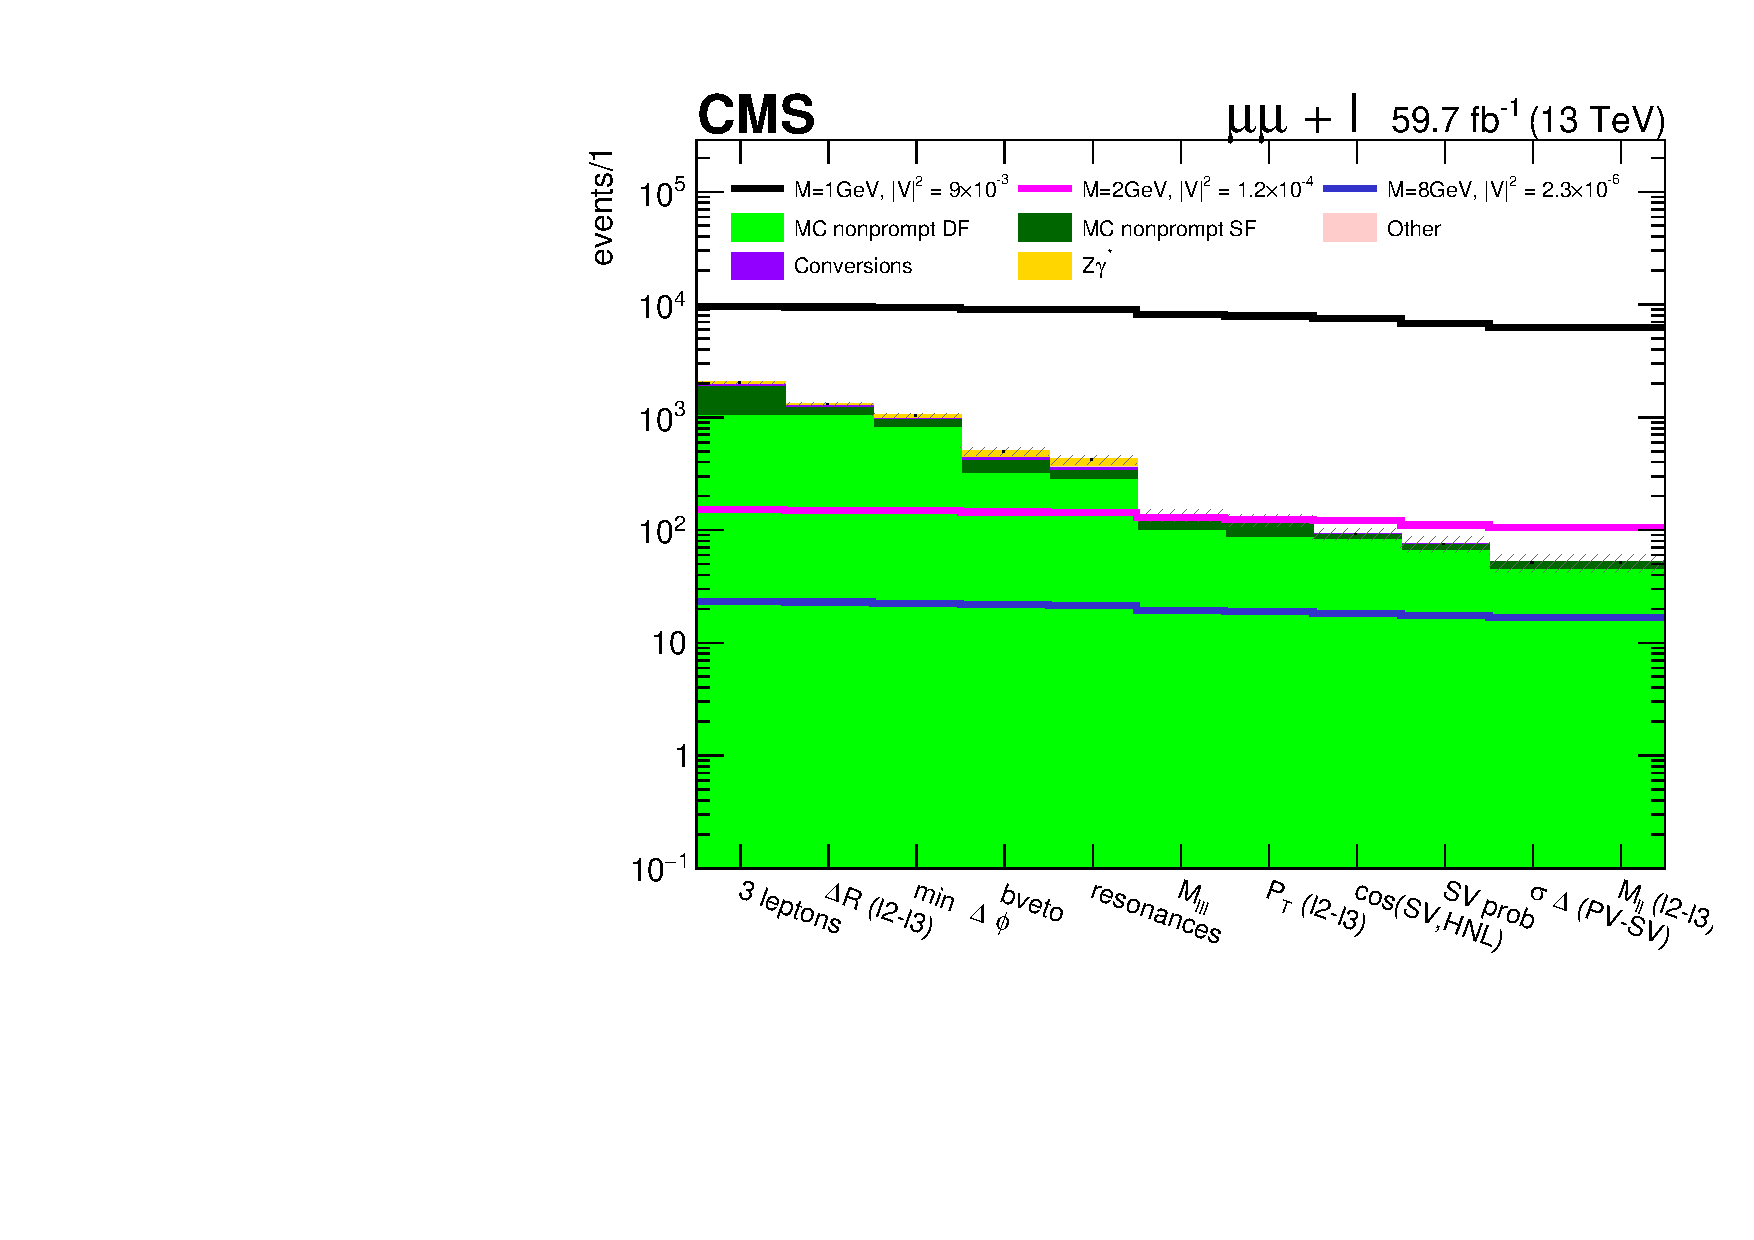
\includegraphics[width=.34\textwidth]{Figures/c6/selection/18/mu_cutflow__0.pdf}}\\
  \makebox[\textwidth]{
   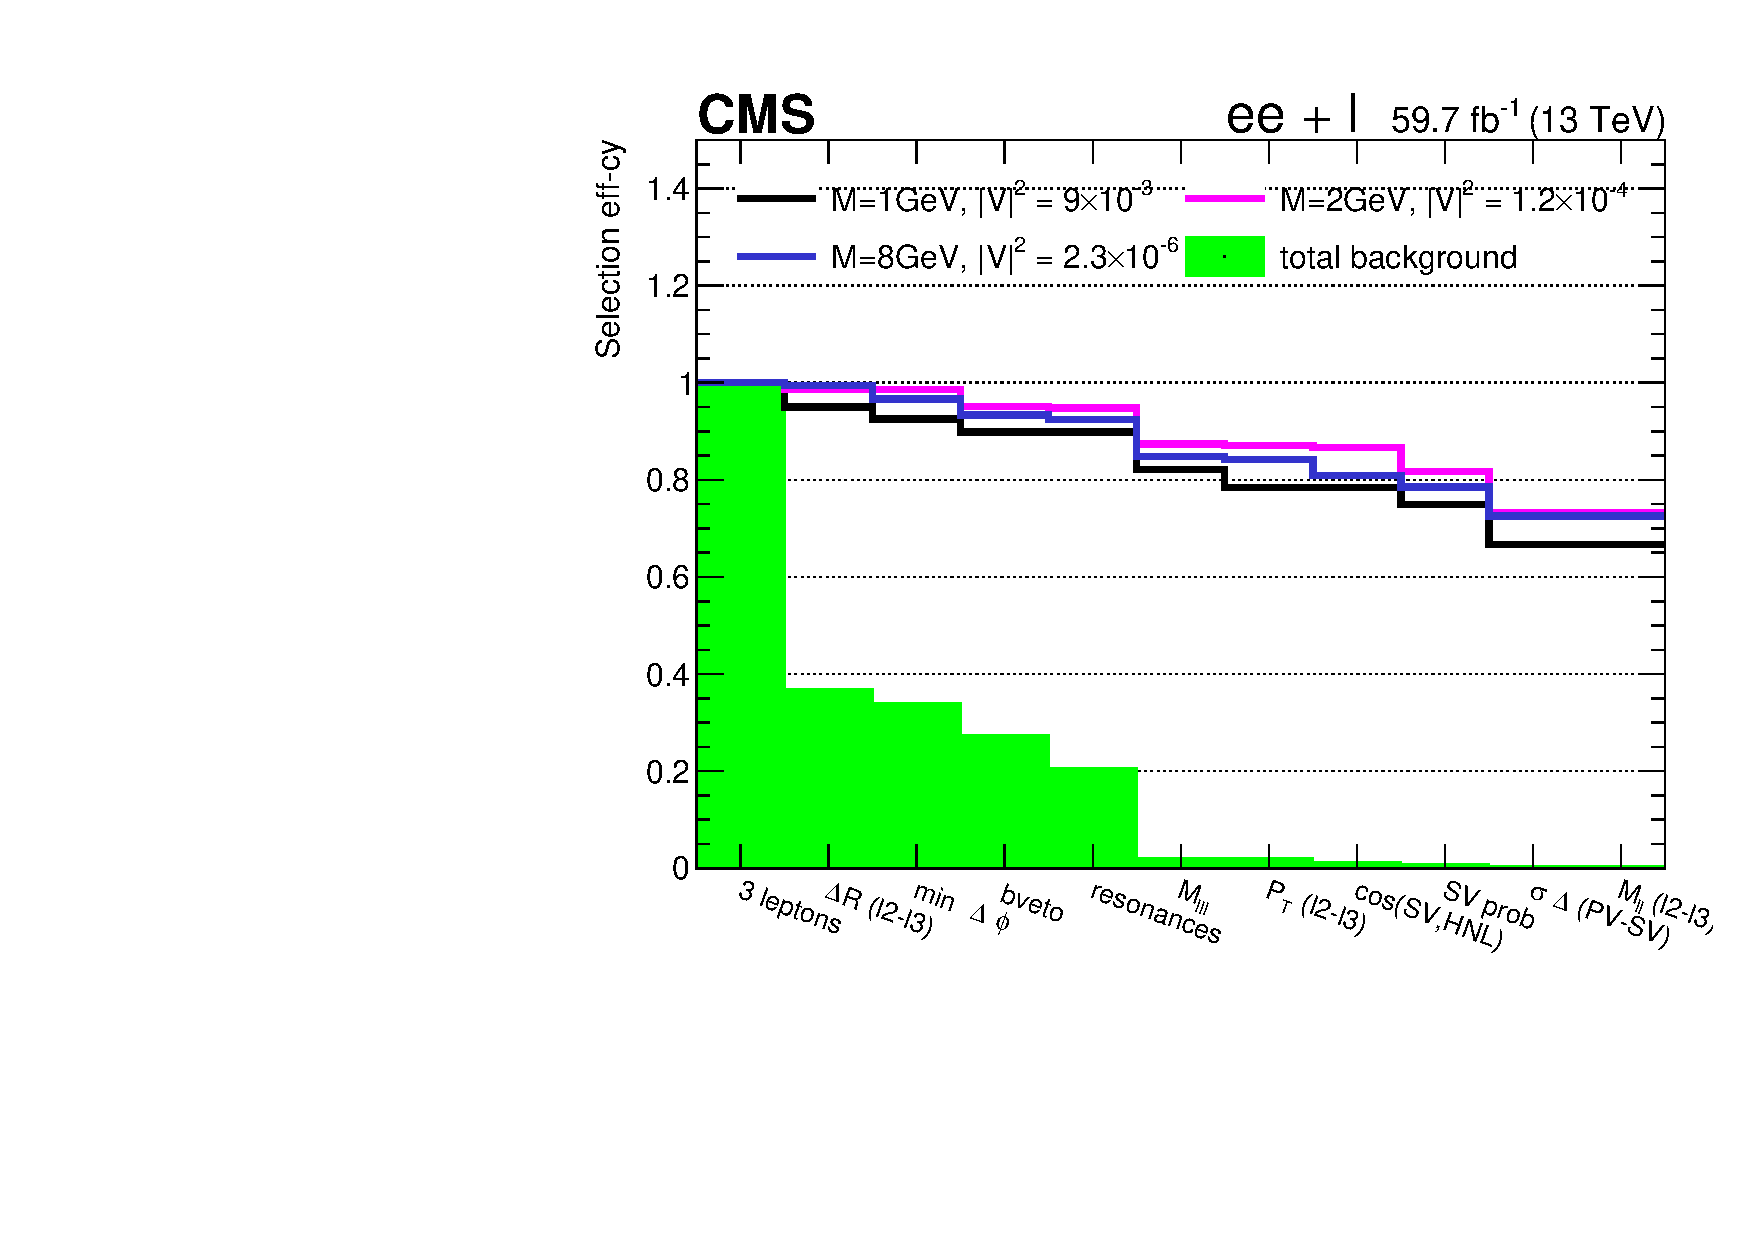
\includegraphics[width=.34\textwidth]{Figures/c6/selection/eff_e_cutflow__0.pdf}
  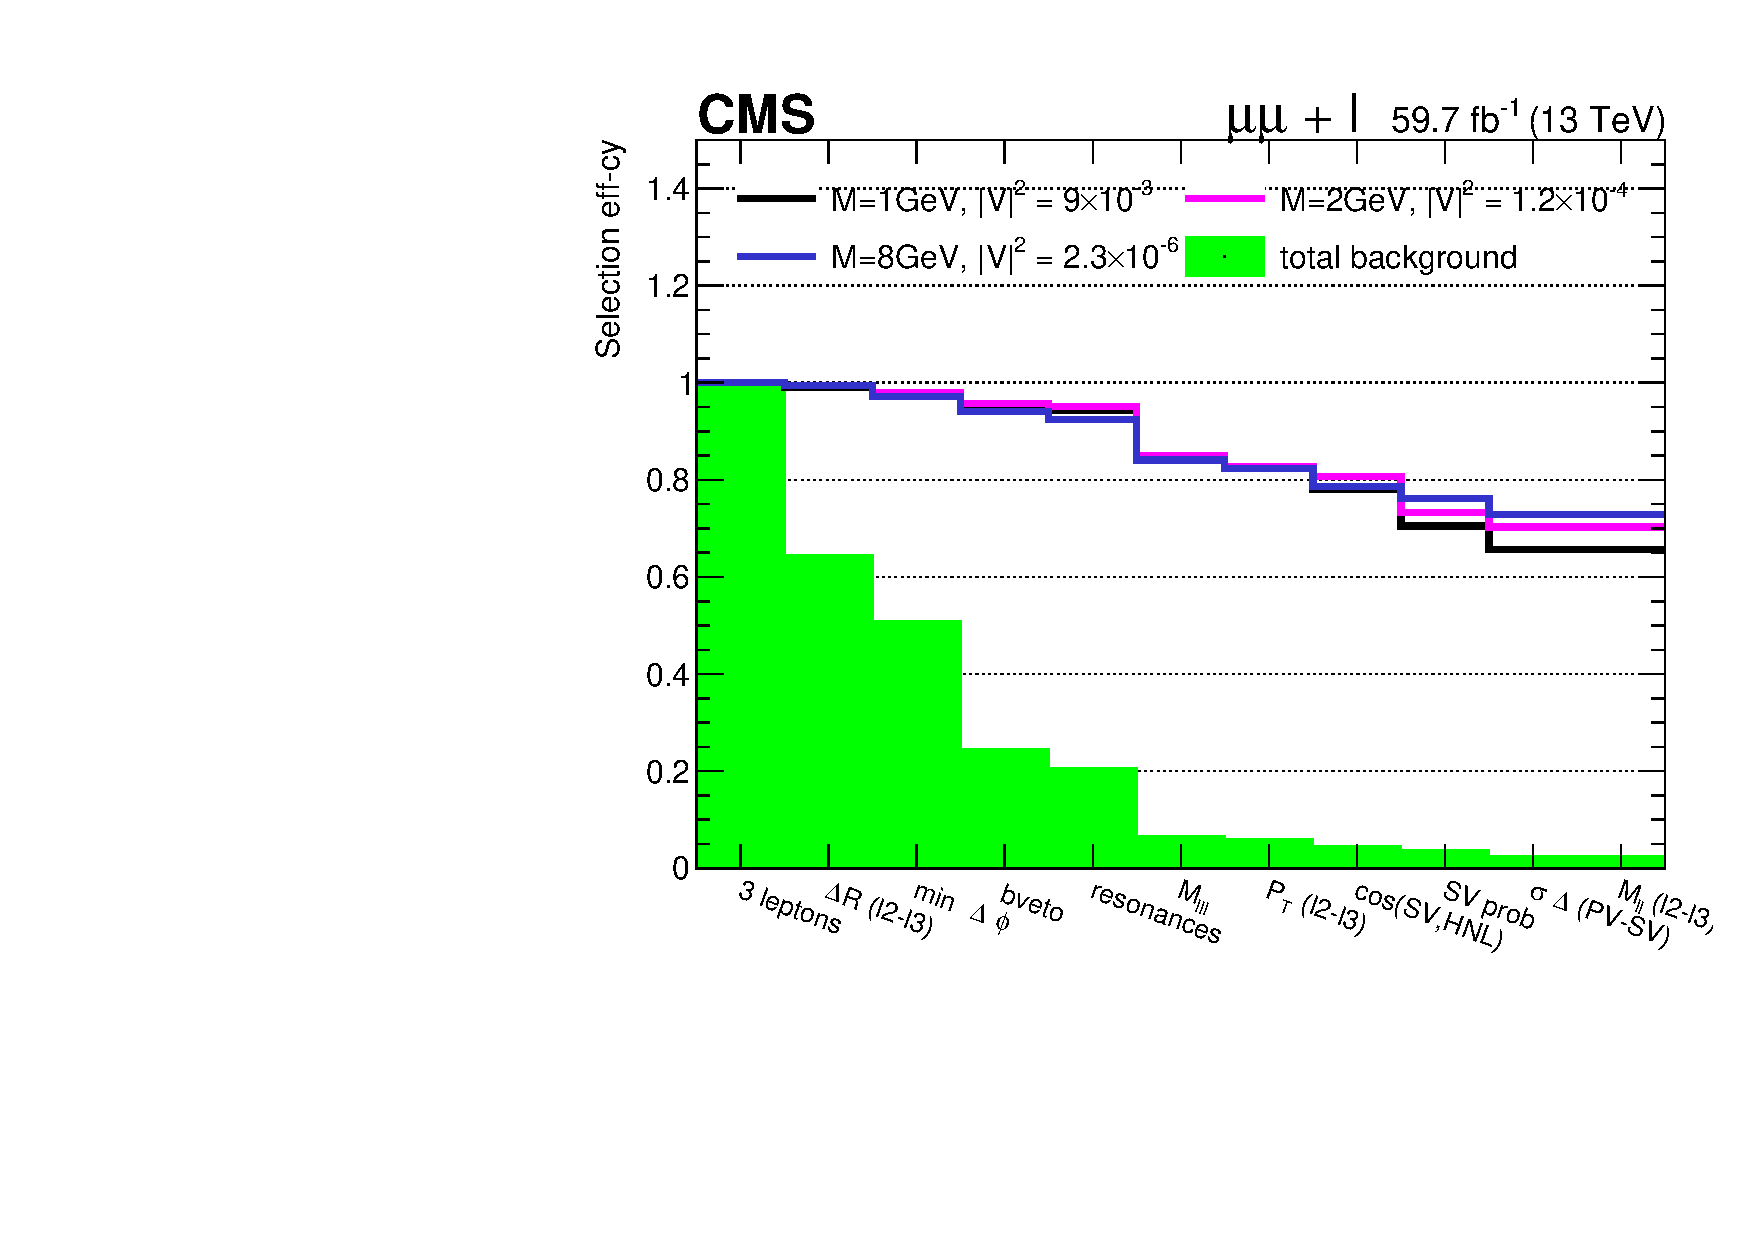
\includegraphics[width=.34\textwidth]{Figures/c6/selection/eff_mu_cutflow__0.pdf}}
  \caption{In the top, cutflow plots showing the full selection applied in simulated backgrounds using the 2018 MC samples,
    in \eex (left) and \mmx (right) final states. In the bottom, cutflow plots but showing the
    efficiency of the selection for the single cut (each bin is $yield_{bin}/yield_{no\:selection}$).
    Signal models for different values of \mhnl and \mixpar
    are shown as empty histograms.}
  \label{fig:cutflow1}
\end{figure}

\begin{figure}[t]
  \noindent
  \makebox[\textwidth]{
 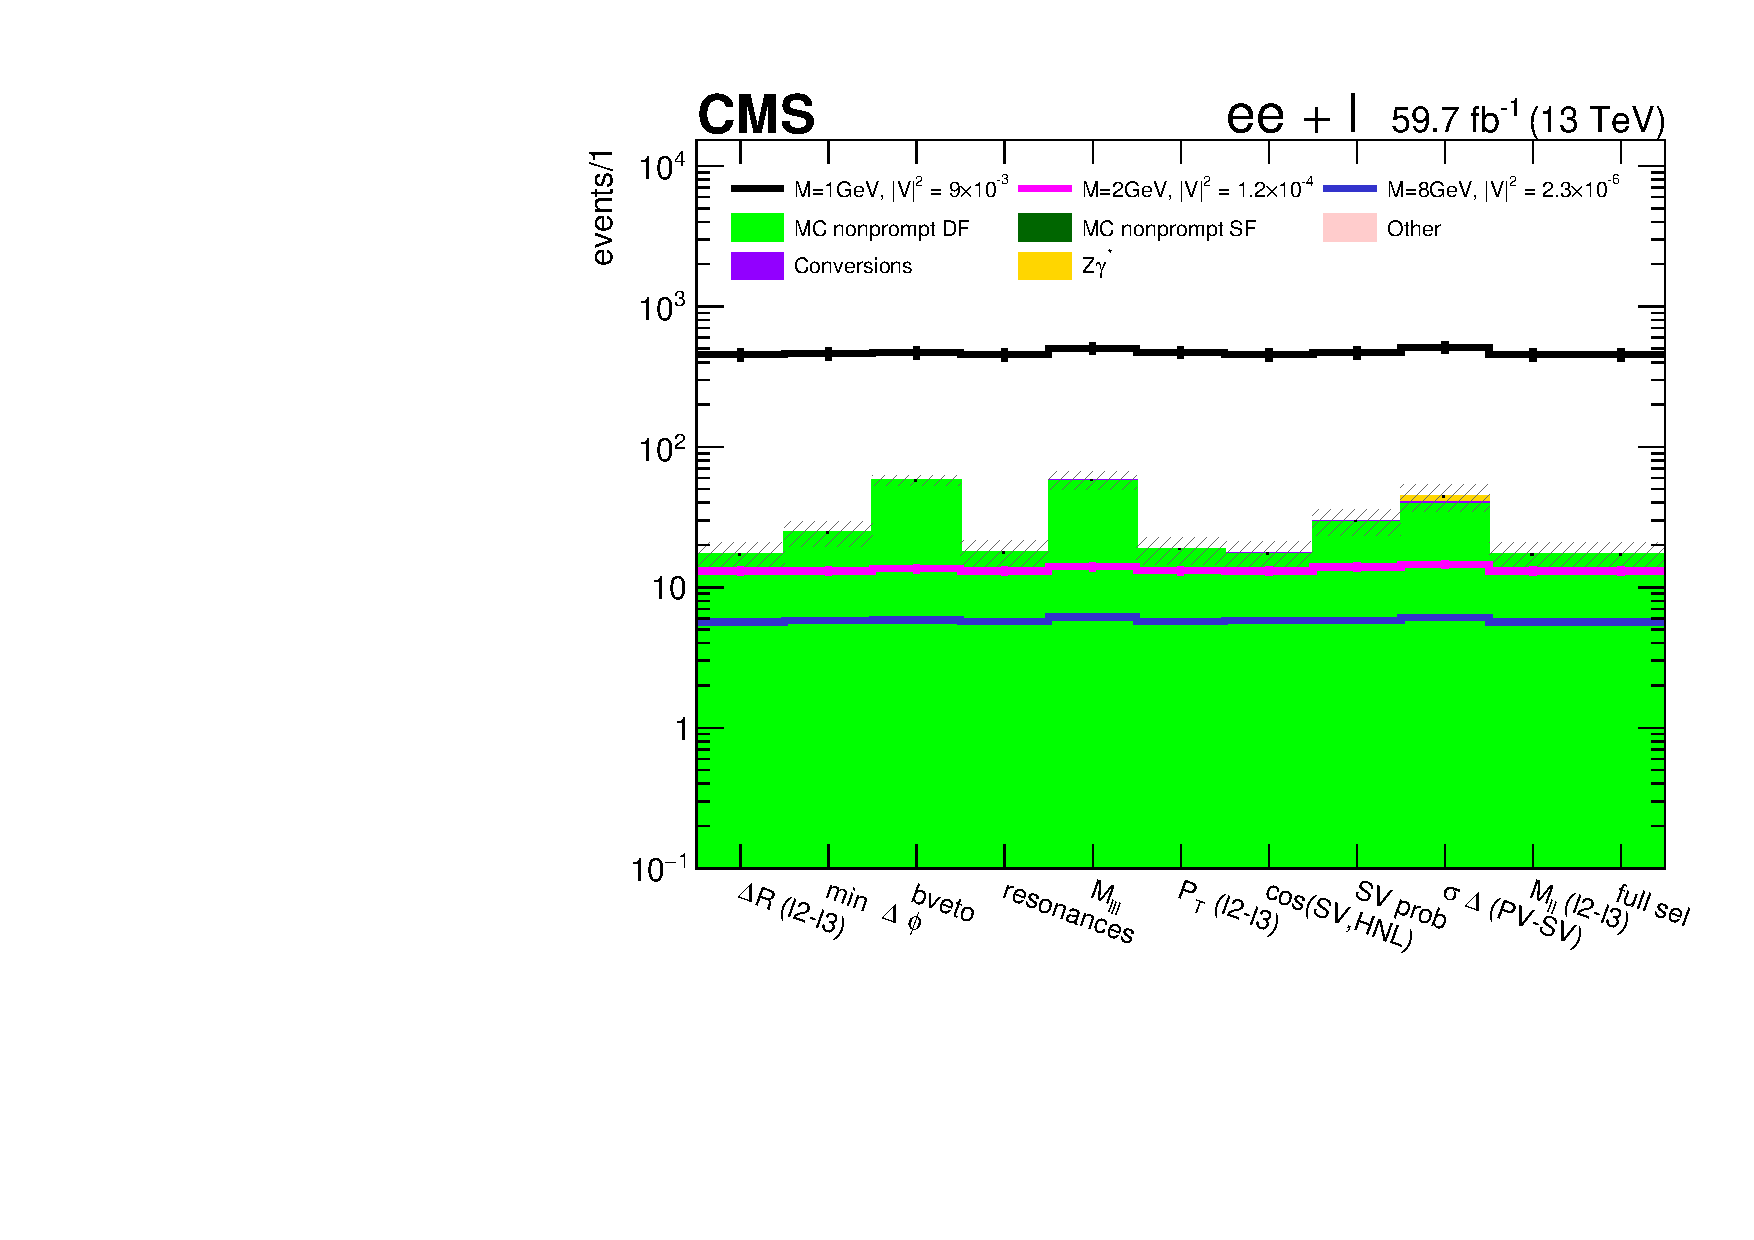
\includegraphics[width=.34\textwidth]{Figures/c6/selection/18/e_cutflow_n_1__0.pdf}
  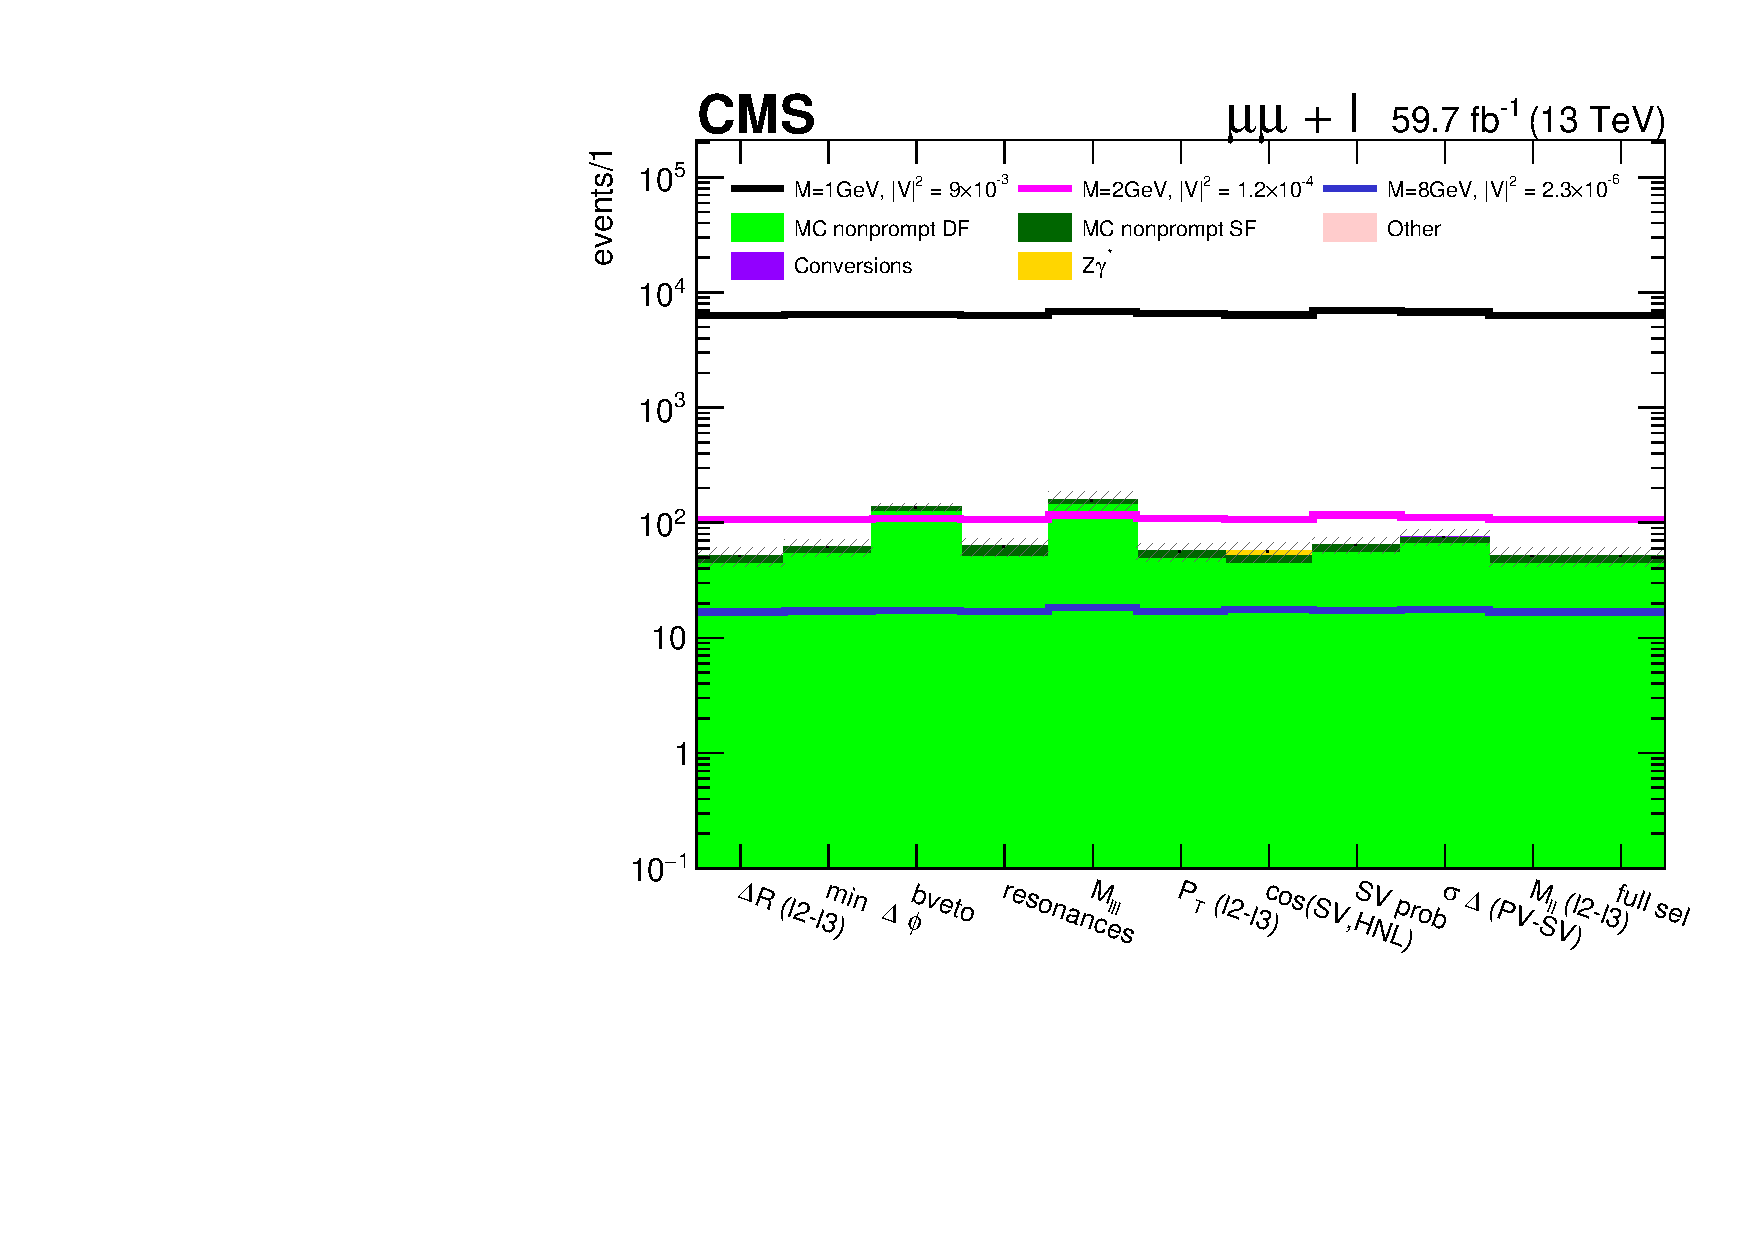
\includegraphics[width=.34\textwidth]{Figures/c6/selection/18/mu_cutflow_n_1__0.pdf}}\\
  \makebox[\textwidth]{
   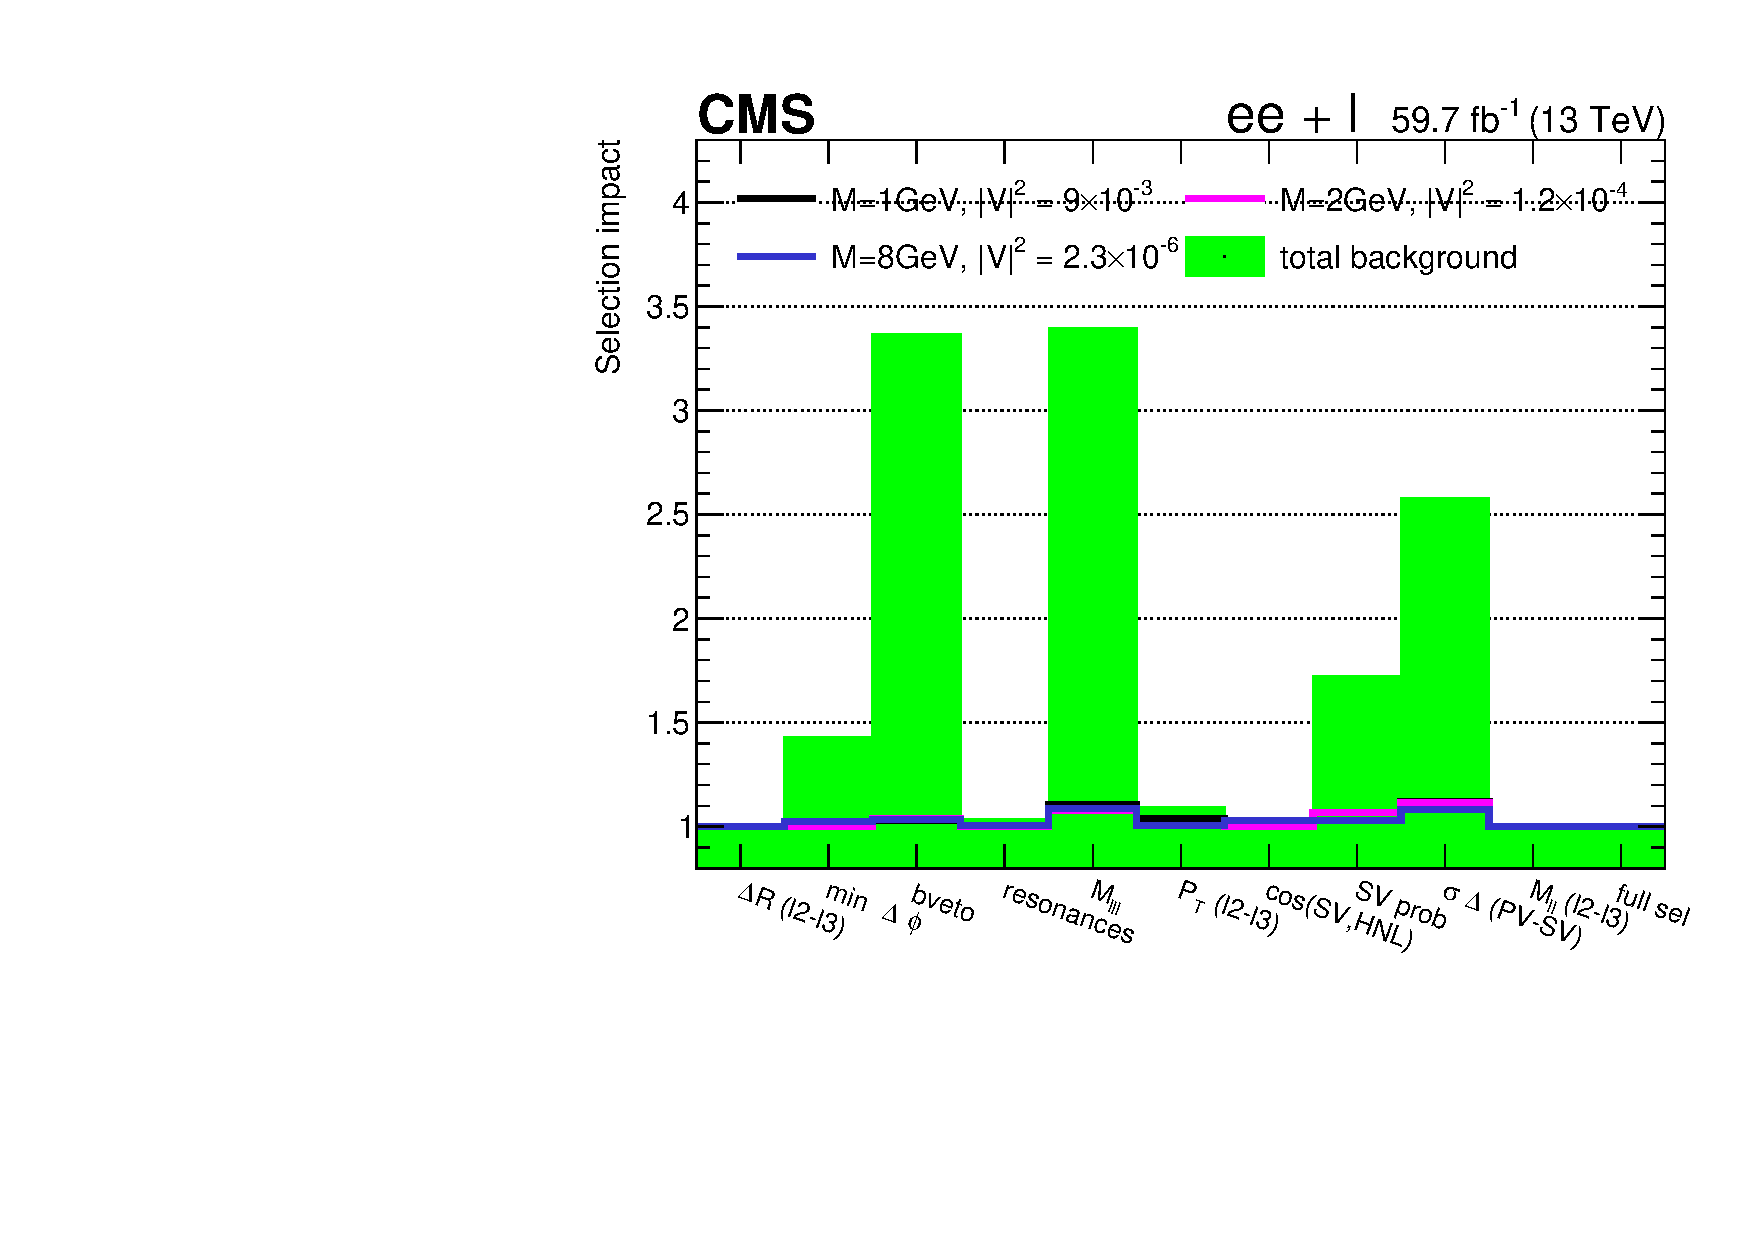
\includegraphics[width=.34\textwidth]{Figures/c6/selection/eff_e_cutflow_n_1__0.pdf}
  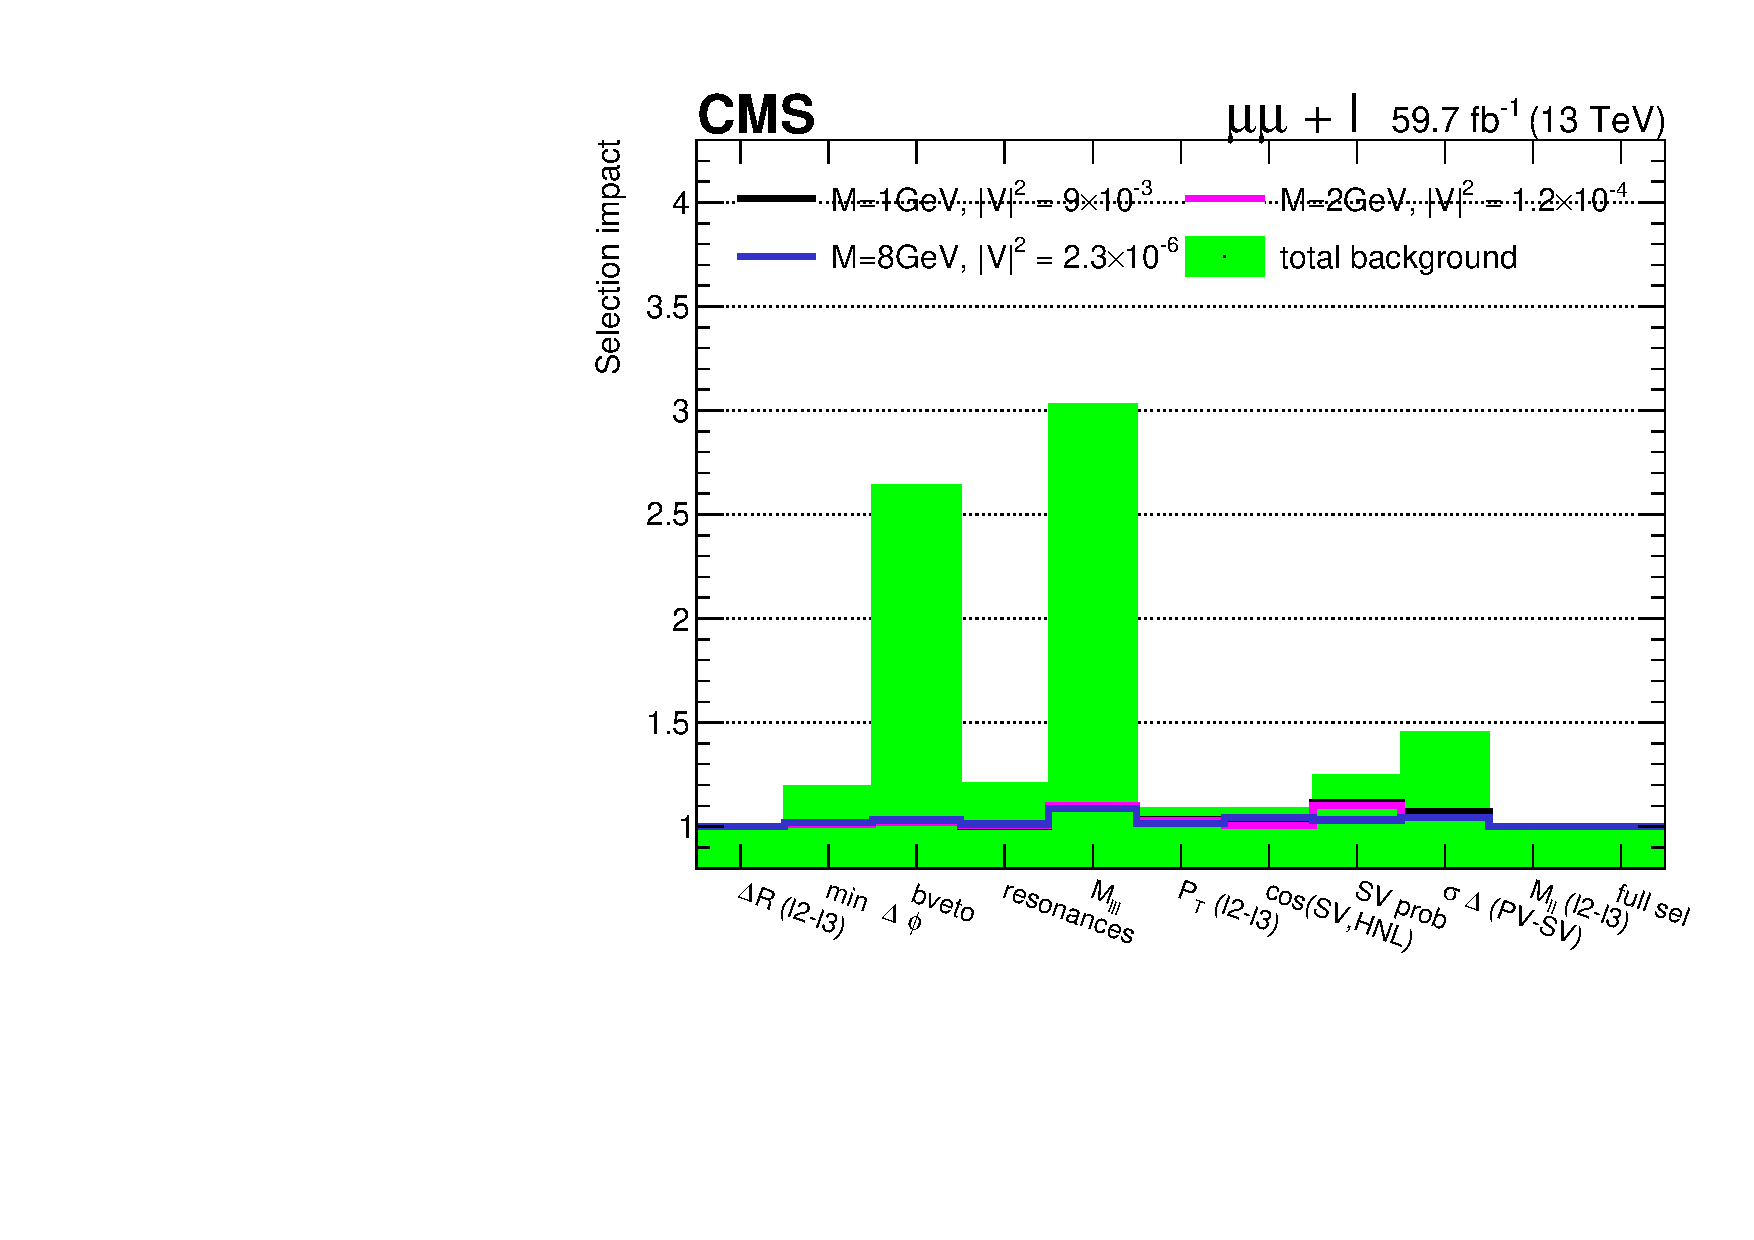
\includegraphics[width=.34\textwidth]{Figures/c6/selection/eff_mu_cutflow_n_1__0.pdf}}
  \caption{In the top, $N-1$ plots showing the real impact of each cut of the full selection in simulated backgrounds using the 2018 MC samples,
    in \eex (left) and \mmx (right) final states. The last bin has the number of events when all the cuts are applied.
    In the bottom, $N-1$ plots but showing the impact in percentage of the single cut (each bin is $yield_{bin}/yield_{full\:selection}$).
    Signal models for different values of \mhnl and \mixpar
    are shown as empty histograms.}
  \label{fig:cutflow2}
\end{figure}
\vspace{2mm}

%One key feature of an analysis involving displaced vertices is the
%high sensitivity and low statistics of regions with large
%displacements.
Figure~\ref{fig:reco_displ} shows the transverse
distance of the SV from the PV, \Deltwod, for events
passing the full baseline selection.
\begin{figure}[h]
  \noindent
  \makebox[\textwidth]{
  \includegraphics[width=.28\textwidth]{Figures/c6/selection/18/e_DeltaPV_SV_2D_zomm__final.pdf}
  \includegraphics[width=.28\textwidth]{Figures/c6/selection/18/mu_DeltaPV_SV_2D_zomm__final.pdf}
  \includegraphics[width=.28\textwidth]{Figures/c6/selection/18/e_M_ll_l2_l3_zoom__final.pdf}
  \includegraphics[width=.28\textwidth]{Figures/c6/selection/18/mu_M_ll_l2_l3_zoom__final.pdf}}
  \caption{\Deltwod (left), and $M_{\ltwo \lthree}$ (right) in events
    passing the baseline selection of Table~\ref{tab:baselinesel}}
  \label{fig:reco_displ}
\end{figure}

In the region of large displacement, the sensitivity of the analysis
greatly increases, with a relatively low abundance of nonprompt lepton
background and being virtually free of prompt lepton background
contributions. This represents the key feature of the analysis.
On the contrary, signals with higher masses are short-lived \hnl
decaying in low displacement regions, where both the prompt and
nonprompt lepton contributions are large, similarly to the previous
CMS search presented in Chapter~\ref{Chapter5}.
Although the sensitivity of the analysis strongly depends on the
secondary vertex displacement, no selection is applied on this
variable. This is due to the fact that both small and large
displacement regions are interesting for the search. The small
displacement region represents the region of the previous CMS search
and can be used to cross-check its results, while the large
displacement region provides the highest sensitivity to long-lived
HNLs. 
Thus, the final signal region will be divided into bins of different
displacement, in addition to the invariant mass of \ltwo and \lthree,
\mtwol (fig.~\ref{fig:reco_displ}).\\

The residual background, dominated by \Xg,
$\PZ/\PGg^{\ast}+\mathrm{jets}$, and top processes, accumulates at low
displacement. The HNL signal models populate higher \Deltwod bins, depending on \mhnl and \mixpar. In particular, \Deltwod
is found to provide the best discrimination between signal and
background, and among different signal models.
Therefore we select four event categories, based on the value of
\Deltwod, with different sensitivities for different signal
scenarios:
$\Deltwod<0.5$\cm (fully background dominated), $0.5<\Deltwod<1.5$\cm,
$1.5<\Deltwod<4$\cm and $\Deltwod>4$\cm.\\
In addition, the events are split into 3 different final states. In case 
the muon coupling is been probed the 3 final states are $\mu\mu\mu$,  $\mu^{\mp}\mu^{\pm} e$ 
and $\mu^{\pm}\mu^{\pm}e$; in case of electron coupling the 3 final states
are: $eee$,  $e^{\mp}e^{\pm}\mu$ and $e^{\pm}e^{\pm}\mu$. This latter categorization
is necessary to provide separated limits for the case of LNC ($\mu^{\mp}\mu^{\pm} e$ and $e^{\mp}e^{\pm}\mu$)
and for the case LNV ($\mu^{\pm}\mu^{\pm} e$ and $e^{\pm}e^{\pm}\mu$), (see Sec.~\ref{sec:lnv_lnc}).
The different categories are also characterized by different
background levels and composition, thus providing different
sensitivities.

Finally we notice that the top background processes, where \ltwo and
\lthree are typically produced in the semi-leptonic decay of $B$
hadrons, populate a region of $\mtwol<4$\GeV, and are basically absent
at higher dilepton masses. Therefore we further split the data into
two categories: $\mtwol<4$\GeV and $\mtwol>4$\GeV. 
\vspace{12mm}

Due to the lack of statistic (in background) at large displacement bins for high mass region, it has been decided to reduce the number of bins 
in the following way:

\begin{itemize}
\setlength\itemsep{-0.5em}
\item for $\mtwol<4$\GeV
  \begin{itemize}
    \setlength\itemsep{-0.4em}
    \item $\Deltwod<0.5$\cm
    \item $0.5<\Deltwod<1.5$\cm
    \item $1.5<\Deltwod<4$\cm
    \item $\Deltwod>4$\cm
  \end{itemize}  
\item for $\mtwol>4$\GeV
\begin{itemize}
    \setlength\itemsep{-0.4em}
    \item $\Deltwod<0.5$\cm
    \item $\Deltwod>0.5$\cm
  \end{itemize}  
\end{itemize}

\comm{
All the distributions previously shown contain background predictions using only MC samples and 
do not have any data points.
At this stage of the analysis process we do not want to show any data-yield since it is not clear yet if 
the background estimation using only MC can predict well the behavior of the data. To ensure so, 
we should first check in regions orthogonal wrt signal region if the MC can predict the data; if it is not the case 
it is important to find a way to predict the contribution of the background using directly data: data-driven estimation.

All the distributions previously shown contain background predictions using only the 2018 MC samples; 2016 and 2017 can be found in Appendix~\ref{app:appendix_MC_2017_2018}.}
\clearpage
%%%%%%%%%%%%%%%%%%%%%%%%%%%%%%%%%%%%%%%%%%%%%%%%%%%%
%%%%%%%%%%%%%%%%%%%%%%%%%%%%%%%%%%%%%%%%%%%%%%%%%%%%
%%%%%%%%%%%%%%%%%%%%%%%%%%%%%%%%%%%%%%%%%%%%%%%%%%%%
\section{Background estimation}\label{sec:llbackground}
\subsection{Background composition}

The main SM background processes mimicking the signal final states can be
classified as follows.
\begin{itemize}
\item \textbf{``Fake'' nonprompt leptons (\Pe or \PGm):}
  muons from light-flavor mesons that decay in flight, or electrons from
  unidentified conversions of photons in jets
  can mimic the \displ leptons from the HNL decay, \ltwo and
  \lthree.
  This background is dominated by top-quark and Drell--Yan processes,
  and is measured with the data-driven method described in
  Sec.~\ref{sec:llfakeBkg}.\\
  Fake nonprompt lepton backgrounds can be split into two categories:
  \begin{itemize}
  \item single fake nonprompt leptons:
    a single reconstructed lepton produced via one of the above
    mechanisms, \eg the (semi-)leptonic decay of a meson.
    Multiple single-fake leptons can be found in an event,
    produced in the independent decays of different mesons.
    In this case, the probabilities to select different fake nonprompt
    leptons for the analysis can be treated as uncorrelated, as
    explained in Sec.~\ref{sec:llsingleFakeBkg}.
  \item double fake nonprompt leptons:
    a pair of reconstructed leptons produced in the decay chain of the
    same hadron, typically a $B$ meson (\eg via
    $\PQb\to\ell^-\bar{\PGn}_{\ell}\PQc\to\ell^-\bar{\PGn}_{\ell}\ell^{\prime+}\PGn_{\ell^{\prime}}\PQs$)
    or a quarkonium state (\eg $\JPsi\to\ell^-\ell^+$).
    In such decays the two leptons are manifestly not independent and
    their selection probabilities are correlated.
    Therefore the lepton pair must be treated as a single system, as
    explained in Sec.~\ref{sec:lldoubleFakeBkg}.
  \end{itemize}
\item \textbf{Photon conversions:}
  \PW or \PZ production processes can
  contribute to the trilepton final state when an initial- or
  final-state photon is radiated and interacts with the material of
  the beam pipe or detector, converting into a pair of electrons.
  These processes are sometimes referred to as ``external''
  conversions, as opposed to ``internal'' conversions of virtual
  photons: $\PGg^\ast\to\ell^-\ell^+$ (\lept can be a muon as well, in
  this case).
  If the photon conversion is strongly asymmetric---\ie one electron
  inherits most of the photon momentum and the other has very low
  \pt---, only the more energetic electron is reconstructed and
  identified. E.g., in $\PZ\to\ell^-\ell^+\PGg$ events with an
  asymmetric conversion of the FSR photon, the final state is
  characterized by three leptons with an invariant mass spectrum
  peaking at the nominal \PZ mass.
  This background gives minor contributions
  to final states with at least a nonprompt electron.
  It is estimated from simulation and verified in control regions with
  three leptons peaking at the \PZ mass (Sec.~\ref{sec:conversion}).
  Such conversions are considered as a
  source of a background, as well as an excellent probe for nonprompt
  lepto n efficiency
 measurement, in many searches for displaced vertices.

\item Multibosons and other rare processes with prompt
  leptons:
  processes with multiple bosons (\PW, \PZ, \PGg, \PH) and/or multiple
  top quarks can give rise to final states with three or more prompt
  leptons.
  The largest contribution in this category comes from $\PW\PZ$ and
  $\PZ\PZ$ diboson production, while processes involving more than two
  bosons or top quarks have very small production rates, and can be
  further suppressed by the lepton and \PQb-jet vetoes.
  These processes constitute an almost negligible background and are
  estimated from simulation.
\end{itemize}
 
\subsection{Fake lepton background}\label{sec_llfakelepton}
The fake-lepton background is estimated using the ``tight-to-loose''
method.\\
A general description of the fake-rate method can be found in
Sec.~\ref{sec:tight_loose_method}.\\

Here ``tight'' refers to the tight identification criteria for
\displ leptons (\ltwo, \lthree) listed in
Tables~\ref{tab:electronSelection} and \ref{tab:muonSelection},
while  ``loose'' refers to the corresponding looser selections
(\ie fakeable objects).

The main difference with respect to the HNL-prompt analysis
(Chapter~\ref{Chapter5}) comes from the different source of fake
leptons; here fake leptons are typically found in the proximity of a
jet which is in common for both \ltwo and \lthree. Each loose
lepton is therefore associated to the jet of $\pt>10\GeV$ closest in
\DR, only if $\DR<0.4$.
If two loose leptons 
are either associated to the same jet or have $\DR<0.45$, they are considered double-fake
leptons and treated as a single dilepton system.
In all other cases --- \ie, if the two loose leptons are associated to
different jets and the $\DR>0.45$ ---,
the loose leptons are considered single fakes and (if more than one)
treated independently.

An important clarification has to be made regarding the estimation of 
the fake-lepton background. This prediction only accounts for fake
nonprompt (``displaced'', \ltwothree) leptons. The contribution from
fake prompt (\ie \lone) leptons is expected to be very small, on
account of the much higher probability for fake \ltwo and \lthree to
pass the tight \displ selection. This assumption has been verified in
MC using the information at generated level (MC truth); at the
beginning of the selection only 1\textperthousand\ background
events have nonprompt \lone, at the end of the selection all \lone
leptons are prompt leptons. 
For this reason, the contribution from fake \lone is neglected.

\subsubsection{Estimation of double-fake background}
\label{sec:doubleFakeBkg}

Events in the application region are classified as double-fake
background if the two nonprompt leptons are either associated to the same
jet or the distance between them is $\DR<0.45$, and at least one of them is loose-not-tight.
In the first case (same jet associated), \ptm is estimated using the \pt of the associated
jet, $\ptm=\ptj$, calibrated using jet energy corrections (JEC, see
Sec.~\ref{sec:jet}) after subtracting the \pt of the two leptons:
\begin{linenomath}
  \begin{equation}
    \label{eq:ptjet}
    \ptm = \ptj =
    \left(\pt^{\mathrm{raw\,jet}}-\pt^{\ltwo}-\pt^{\lthree}\right)\times\mathrm{JEC}
    \;+\; \pt^{\ltwo} \;+\; \pt^{\lthree}.
  \end{equation}
\end{linenomath}
In this formula all the \pt are 4-vectors.
Similar is the case when the distance between them is $\DR<0.45$:
\begin{linenomath}
  \begin{equation}
    \label{eq:ptjet_45}
    \ptm = \ptj = p^{jet,2}_T + p^{jet,3}_T 
  \end{equation}
\end{linenomath}
where the $p^{jet,i}$ is the jet associated to the lepton \emph{i} and then corrected using the JEC right correction:
\begin{linenomath}
  \begin{equation}
    \label{eq:ptjet_45_single}
    p^{jet,i} = \left(\pt^{\mathrm{raw\,jet_i}}-\pt^{\ell_{i}}\right)\times\mathrm{JEC}\;+\; \pt^{\ell_i} .
  \end{equation}
\end{linenomath}

Double fake rates (\dfr) are parametrized and applied as a
function of the \pt of the associated jet:
$\dfr=\dfr(\ptj)$.
The definition of the measurement region is similar to that of the
signal region, with the following differences:
\begin{itemize}
\item the two nonprompt leptons, \ltwo and \lthree, are selected with
  the loose identification criteria (see
  Tables~\ref{tab:electronSelection} and \ref{tab:muonSelection})
  and must be either associated to the same jet or have $\DR<0.45$;
\item a \PQb-tagged jet with $\pt>25$\GeV must be present (not
  necessarily the same that \ltwo and \lthree are associated to).
\end{itemize}
The requirement of a \PQb-jet enriches the sample in top-quark
backgrounds, which are the main source of double-fake leptons, see Table~\ref{tab:measurement_sel}.
Events in this measurement region have two loose (\emph{fakeable object}) nonprompt leptons, of
which zero, one, or both can be tight.
\begin{table}[h!]
  \centering
  \caption{\label{tab:measurement_sel} Measurement region selection requirements
    for double fake.}
    \begin{tabular}{l|l}
    \hline
    Variable     & Requirement       \\
    \hline
    \hline
    N. \PQb jets & $\geq 1$              \\
    \mtwol in $\Pe\Pe\Pe$& $> 0.5$\GeV              \\ 
    resonance vetoes & applied      \\
    \hline
   %% \mthreel  and  N. \PQb jets  & ($<50$\GeV or $>80$\GeV N.\PQb jets= 0) OR  (N.\PQb jets $\neq$ 0)\\
     \hline
     \mthreel in $\Pe\Pe\Pe$ and $\PGm\PGm\Pe$ OS & $<80$\GeV or $>101$\GeV \\
      \mtwol in $\Pe\Pe\Pe$& $> 0.5$\GeV              \\ 
    \hline
    \hline 
  \end{tabular}
\end{table}

The double fake rate \dfr is defined as the fraction of events in this
region where both nonprompt leptons are tight.
Figure~\ref{fig:dFR_ptjet_16}(top) shows
the measured values of \dfr for events with two electrons, an electron
and a muon, and two muons, respectively, as a function of \ptj.
Figure~\ref{fig:dFR_ptjet_16}(bottom) shows
the measured values of \dfr for events with two electrons, an electron
and a muon, and two muons, respectively, as a function of \Deltwod. The \Deltwod bins are the four bins chosen for the SR in order to evaluate 
with is the dependance of the \dfr wrt the displacement of the SV of the \hnl decay. 

\begin{figure}[h]
  \noindent
\makebox[\textwidth]{
  \includegraphics[width=.35\textwidth]{Figures/c6/backgrounds/FR/dFR/16/c_LeptonPt___eta_FR1.pdf}
  \includegraphics[width=.35\textwidth]{Figures/c6/backgrounds/FR/dFR/17/c_LeptonPt___eta_FR1.pdf}
  \includegraphics[width=.35\textwidth]{Figures/c6/backgrounds/FR/dFR/18/c_LeptonPt___eta_FR1.pdf}}
  \noindent
\makebox[\textwidth]{\includegraphics[width=.35\textwidth]{Figures/c6/backgrounds/FR/dFR/16/c_displacement_SR___eta_FR1.pdf}
  \includegraphics[width=.35\textwidth]{Figures/c6/backgrounds/FR/dFR/17/c_displacement_SR___eta_FR1.pdf}
  \includegraphics[width=.35\textwidth]{Figures/c6/backgrounds/FR/dFR/18/c_displacement_SR___eta_FR1.pdf}}
  \caption{Double fake-lepton rates measured in 2016/17/18 (left,
    middle, right) data as a function of \ptj (top) and \Deltwod (bottom),
    for events with two electrons (black), with
    an electron and a muon (red), and with two muons (blue).}
  \label{fig:dFR_ptjet_16}
\end{figure}

The application region for double-fake lepton backgrounds (dFR)
is defined using the same selection as the signal region (see
Table~\ref{tab:baselinesel}), but with one or two loose-not-tight
nonprompt leptons that either be associated to the same jet or have $\DR<0.45$. 
The background from double-fake leptons in the signal region is
estimated from the event yields in the application region dFR using
the formula
\begin{linenomath}
  \begin{equation}
    \label{eq:dFRbkg}
    N_{\mathrm{dFR}}^{\mathrm{sig}} ~=~ 
    \sum_i\frac{\dfr(\ptjs{i})}{1-\dfr(\ptjs{i})}\;,
  \end{equation}
\end{linenomath}
where the sum runs over all the events in dFR, with jet transverse momentum \ptcs{i}.

\subsubsection{Estimation of single-fake background}
\label{sec:singleFakeBkg}

The measurement of the single-fake background exaclty follows the same
procedure as the one explained in Sec.~\ref{sec:singleFR}. Thus, to
avoid repetitions, only the final measured FR are presented here; for
additional plots see Appendix~\ref{AppendixA}, Sec.~\ref{app:sfr}.

Figure~\ref{fig:sfr_data} shows the measured
values of \sfr for electrons and muons in simulation and in data,
respectively, as a function of \ptc and in different \abseta bins.


\begin{figure}[h]
  \centering
  \includegraphics[height=6.4cm, width=7.0cm]{Figures/c6/backgrounds/FR/sFR/data/electrons.pdf}
  \hfill{}
  \includegraphics[height=6.4cm, width=7.0cm]{Figures/c6/backgrounds/FR/sFR/data/muons.pdf}\\
  \caption{Single fake rates measured in 2016 data for electrons (left) and
    muons (right) as a function of \ptc, for \abseta ranges $[0,0.8]$
    (top), $[0.8,1.479]$ (middle), and $[1.479,2.5]$ (bottom).}
  \label{fig:sfr_data}
\end{figure}

Figures~\ref{fig:sfr_dxy} show that \sfr values are fairly independent
of the lepton \dxy.
\begin{figure}[h]
  \centering
  \includegraphics[width=.48\textwidth]{Figures/c6/backgrounds/FR/sFR/QCD/dxy_ele_eta1_FR2.pdf}
  \hfill{}
  \includegraphics[width=.48\textwidth]{Figures/c6/backgrounds/FR/sFR/QCD/dxy_mu_eta1_FR2.pdf}\\
  \includegraphics[width=.48\textwidth]{Figures/c6/backgrounds/FR/sFR/QCD/dxy_ele_eta2_FR2.pdf}
  \hfill{}
  \includegraphics[width=.48\textwidth]{Figures/c6/backgrounds/FR/sFR/QCD/dxy_mu_eta2_FR2.pdf}\\
  \includegraphics[width=.48\textwidth]{Figures/c6/backgrounds/FR/sFR/QCD/dxy_ele_eta3_FR2.pdf}
  \hfill{}
  \includegraphics[width=.48\textwidth]{Figures/c6/backgrounds/FR/sFR/QCD/dxy_mu_eta3_FR2.pdf}
  \caption{Single fake rates obtained in 2016 simulation for electrons
    (left) and muons (right) as
    a function of \dxy, for \abseta ranges $[0,0.8]$ (top),
    $[0.8,1.479]$ (middle), and $[1.479,2.5]$ (bottom).}
  \label{fig:sfr_dxy}
\end{figure}























\clearpage
\section{Corrections and efficiencies}
\section{Systematic uncertainties}
\section{Results}
\subsection{Statistical analysis}
\subsection{Limits on $V_{Nl}$: Dirac HNL}
\subsection{Limits on $V_{Nl}$: Majorana HNL}
\subsection{Limits on $V_{Nl}$: Tau coupling}

\subsection{Summary}

